\documentclass[a4paper, thm-restate]{book}
\usepackage{graphicx}
\usepackage{caption}
\usepackage{subcaption}
\usepackage{amsmath}
\usepackage{amsfonts}
\usepackage{amsthm}
\usepackage{amssymb}
\usepackage{color}
\usepackage{enumitem}
\usepackage{multicol}
\usepackage[ruled,vlined,noend,resetcount,algochapter]{algorithm2e}
\usepackage{verbatim} 
\usepackage{url}  
\usepackage{esvect}
\usepackage[advantage,operators,primitives,oracles,logic,sets,ff,mm,keys,adversary,lambda,notions,probability,asymptotics]{cryptocode}
\usepackage[bookmarks,bookmarksopen,bookmarksdepth=2]{hyperref}
\usepackage[backend=bibtex,style=numeric,maxnames=50, abbreviate=true]{biblatex}
\usepackage[english, greek]{babel}
\usepackage{alphabeta}

\addbibresource{refs.bib}
% \pagestyle{myheadings}

% language 
\newcommand{\sle}{\selectlanguage{english}}
\newcommand{\slg}{\selectlanguage{greek}}

\newcommand{\ddh}{\textup{\textsf{DDH}}}
\renewcommand{\ro}{\mathcal{RO}}

% //TODO: put a macro for sets of accounts!

\providecommand{\snap}{\state}
\newcommand{\params}{\textup{\texttt{{pp}}}} % public parameters
\newcommand{\instate}{\state_0} % initial state produced by setup
\providecommand{\auditinfo}{{\textup{\pcalgostyle{auditInfo}}}}

% Algorithms for UPK
\providecommand{\setup}{\pcalgostyle{Setup}}
\providecommand{\kgen}{\pcalgostyle{KGen}}
\providecommand{\upd}{\pcalgostyle{Update}}
\providecommand{\verkp}{\pcalgostyle{VerifyKP}}
\providecommand{\verupd}{\pcalgostyle{VerifyUpdate}}

% Main algorithms
\providecommand{\reg}{\pcalgostyle{Register}}
\providecommand{\verreg}{\pcalgostyle{VerifyRegister}}
\providecommand{\createAcct}{\pcalgostyle{CreateAcct}}
\providecommand{\deleteAcct}{\pcalgostyle{DeleteAcct}}
\providecommand{\vercreateAcct}{\pcalgostyle{VerifyCreateAcct}}
\providecommand{\verdeleteAcct}{\pcalgostyle{VerifyDeleteAcct}}
\providecommand{\trans}{\pcalgostyle{Trans}}
\providecommand{\vertxn}{\pcalgostyle{VerifyTrans}}
\providecommand{\audit}{\pcalgostyle{Audit}}
\providecommand{\vera}{\pcalgostyle{VerifyAudit}}
\providecommand{\applytxn}{\pcalgostyle{ApplyTrans}}
\providecommand{\applyreg}{\pcalgostyle{ApplyRegister}}

%Auxilary functions
\providecommand{\vercom}{\pcalgostyle{VerifyCom}}
% \providecommand{\genacct}{\pcalgostyle{GenAcct}}
\providecommand{\veract}{\pcalgostyle{VerifyAcct}}
\providecommand{\updacc}{\pcalgostyle{UpdateAcct}}
\providecommand{\verupdacc}{\pcalgostyle{VerifyUpdateAcct}}
\providecommand{\genuser}{\pcalgostyle{GenUser}}
\providecommand{\veruser}{\pcalgostyle{VerifyUser}}
\providecommand{\upduser}{\pcalgostyle{UpdateUser}}
\providecommand{\verupduser}{\pcalgostyle{VerifyUpdateUser}}
\providecommand{\newacc}{\pcalgostyle{NewAcct}}
\providecommand{\vernewacc}{\pcalgostyle{VerifyNewAcct}}

% Variables names
\newcommand{\msg}{ \mathtt{m} }
% \newcommand{\rnd}{ \rand }
\newcommand{\rand}{\mathtt{r}}
\newcommand{\id}{{\textup{\texttt{id}}}} % user "real" credentials
\newcommand{\user}{\textup{\textsf{user}}}
\newcommand{\acct}{\textup{\textsf{acct}}}
\newcommand{\accttodelete}{\acct_\textsf{D}}
\newcommand{\accttotransfer}{\acct_\textsf{C}}
\newcommand{\userinfo}{\textup{\textsf{userInfo}}} % tupple in userSet
\newcommand{\varbl}{\textup{\texttt{{bl}}}}
\newcommand{\varout}{\textup{\texttt{{out}}}}
\newcommand{\varin}{\textup{\texttt{{in}}}}
\newcommand{\outdelete}{\varout_\textsf{D}}
\newcommand{\indelete}{\varin_\textsf{D}}
\newcommand{\inpk}{\textup{\texttt{pk}}_{0}} % initial public key
\newcommand{\numaccs}{\textup{\texttt{\#accs}}}
\newcommand{\srlimit}{\textup{\texttt{a}}_{max}} 
\newcommand{\vtof}{\textup{\texttt{{v}}}_{t}} % value send to tax office
\newcommand{\num}{{\textup{\texttt{n}}}} % number of accounts in the inputs of txns
\newcommand{\inputs}{{\textup{\texttt{inputs}}}} % inputs of txns
\newcommand{\outputs}{{\textup{\texttt{outputs}}}} % outputs of txns
\newcommand{\aux}{{\textup{\texttt{aux}}}} % auxilary data to audit
\newcommand{\com}{\texttt{com}} % a commitment to a value-we don't know the value

\newcommand{\snum}{{\textup{\texttt{s}}}} % number of senders
\newcommand{\rnum}{{\textup{\texttt{t}}}} % number of recipients

% Transactions
\newcommand{\txn}{\textup{\textsf{tx}}}
\newcommand{\txnca}{\textup{\textsf{tx}}_\textsf{CA}}
\newcommand{\txnda}{\textup{\textsf{tx}}_\textsf{DA}}

% Commitments
\newcommand{\comm}[1]{\fbox{$#1$}}
\providecommand{\commit}{\pcalgostyle{Commit}}
\newcommand{\verifycom}{\pcalgostyle{VerifyCom}}
\newcommand{\opencom}{\pcalgostyle{OpenCom}}

% Vectors values
\newcommand{\vbl}{\textup{\texttt{{v}}}_{\varbl}}
\newcommand{\vout}{\textup{\texttt{{v}}}_{\varout}}
\newcommand{\vin}{\textup{\texttt{{v}}}_{\varin}}
\newcommand{\vnumaccs}{\textup{\texttt{{v}}}_{\#accs}}
\renewcommand{\v}{\texttt{v}} % a 'v' of the same style

% user and utxo set
\newcommand{\usersset}{\pcalgostyle{UserSet}}
\newcommand{\utxoset}{\pcalgostyle{UTXOSet}}

% policies
\newcommand{\sendlimit}{\pcalgostyle{slimit}}
\newcommand{\receivelimit}{\pcalgostyle{rlimit}}
% \newcommand{\rate}{\pcalgostyle{rate}}
\newcommand{\open}{\pcalgostyle{open}}
\newcommand{\taxoffice}{\pcalgostyle{to}}
\newcommand{\blacklist}{\pcalgostyle{blacklist}}
\newcommand{\txnlimit}{\pcalgostyle{txlimit}}
\newcommand{\nonpart}{\pcalgostyle{np}}

% security-oracle queries
% \newcommand{\corruptAcctOracle}{\pcalgostyle{CorruptAcct}}
% \newcommand{\corruptUserOracle}{\pcalgostyle{CorruptUser}}
\newcommand{\corruptOracle}{\pcalgostyle{OCorrupt}}
\newcommand{\transOracle}{\pcalgostyle{O}\trans}
\newcommand{\applytxnOracle}{\pcalgostyle{O}\applytxn}
\newcommand{\regOracle}{\pcalgostyle{O}\reg}
\newcommand{\verregOracle}{\pcalgostyle{O}\verreg}
\newcommand{\createAcctOracle}{\pcalgostyle{O}\createAcct}
\newcommand{\deleteAcctOracle}{\pcalgostyle{O}\deleteAcct}
\newcommand{\veraOracle}{\pcalgostyle{O}\vera}
\newcommand{\vercreateAcctOracle}{\pcalgostyle{O}\vercreateAcct}
\newcommand{\auditOracle}{\pcalgostyle{O}\audit}

% security-bookkeeping
\newcommand{\activeacc}{\pcalgostyle{active}}
\newcommand{\inactiveacc}{\pcalgostyle{inactive}}
\newcommand{\status}{\pcalgostyle{status}}
\newcommand{\bookkeepingfunctionality}{\pcalgostyle{bookkeeping}}
\newcommand{\initbookkeeping}{\pcalgostyle{init}}
\newcommand{\updatebookkeeping}{\pcalgostyle{update}}
\newcommand{\countwealth}{\pcalgostyle{totalWealth}}
\newcommand{\findsecretkey}{\pcalgostyle{findSecretKey}}
\newcommand{\verifypolicy}{\pcalgostyle{verifyPolicy}}

% another adversary
\newcommand{\badv}{\mathcal{B}}

% security-corrupt and honest sets of users
\newcommand{\entries}{\pcalgostyle{entries}}
\newcommand{\honest}{\pcalgostyle{honest}}
\newcommand{\corrupt}{\pcalgostyle{corrupt}}
\newcommand{\stateslist}{\pcalgostyle{states}}
% for count wealth of bookkeeping
\newcommand{\honestorcorrupt}{\pcalgostyle{set}}
\newcommand{\type}{\pcalgostyle{type}}

\newcommand{\utxo}{\pcalgostyle{utxo}}

% experiments and advantage
\newcommand{\exper}{\textup{\textsf{Exp}}}
\newcommand{\anonymity}{\textup{anon}}
\newcommand{\theftprevention}{\textup{theft}}
\newcommand{\auditsoundness}{\textup{ausound}}

% Sets and Spaces
\newcommand{\group}{\mathbb{G}}
\newcommand{\msgspace}{\mathcal{M}} 
\newcommand{\randspace}{\mathcal{R}}
\newcommand{\vset}{\mathcal{V}} % space of values for bl, out, in
\newcommand{\anset}{{\mathtt{A}}} % anonymity set
\newcommand{\pset}{\mathtt{P}} % sender & receiver set
\newcommand{\rset}{\mathtt{R}} % receiver set
\newcommand{\sset}{\mathtt{S}} % senders set
\newcommand{\indices}{\mathtt{I}} % indices set
\newcommand{\isset}{\indices_\sset} % indices of sender set
\newcommand{\irset}{\indices_\rset} % indices of receiver set
\newcommand{\ianset}{\indices_\anset} % indices of anonymity set
\newcommand{\blist}{\pcalgostyle{BL}} % blacklist set

% Authorities 
\newcommand{\RA}{\textup{\texttt{{RA}}}}
\renewcommand{\AA}{\textup{\texttt{{AA}}}}
\newcommand{\UU}{\textup{\texttt{{U}}}}

% Auxiliary functions for proof system
\providecommand{\createdelta}{\pcalgostyle{CreateDelta}}
\providecommand{\verdelta}{\pcalgostyle{VerifyDelta}}
\providecommand{\vernonneg}{\pcalgostyle{VerifyNonNegative}}
\providecommand{\upddelta}{\pcalgostyle{UpdateDelta}}
\providecommand{\verupddelta}{\pcalgostyle{VerifyUD}}
\providecommand{\versenderdelta}{\pcalgostyle{VerifyDeltaSender}}
\providecommand{\verrecdelta}{\pcalgostyle{VerifyDeltaReceiver}}

\providecommand{\nizkprove}{\pcalgostyle{NIZK.Prove}}

\newenvironment{boxfig}[2]{%
	\begin{figure}[!]
		\newcommand{\FigCaption}{#1}
		\newcommand{\FigLabel}{#2}
	      \vspace{-0.25cm}
		\begin{center}
			\begin{small}
				\begin{tabular}{@{}|@{~~}l@{~~}|@{}}
					\hline
					\rule[-1.5ex]{0pt}{1ex}\begin{minipage}[b]{\textwidth}
						\vspace{1ex}
						\smallskip
					}{%
				\end{minipage}\\
				\hline
			\end{tabular}
		\end{small}
	    \vspace{-0.35cm}
		\caption{\FigCaption}
	\end{center}
	\vspace{-0.5cm}
\end{figure}
}

\newenvironment{game}[1][htbp]
  {\renewcommand{\algorithmcfname}{Game}% Update algorithm name
   \begin{algorithm}[#1]%
  }{\end{algorithm}}


\title{Privacy and Auditability in Decentralized Payment Systems}
% \author{Γεώργιος Παπαδούλης }
% \date{October 2023}

% \newtheorem{theorem}{Theorem}
\newtheorem{theorem}{Theorem} %[section]
\newtheorem{corollary}{Corollary} %[theorem]
\newtheorem{lemma}[theorem]{Lemma}
\newtheorem{definition}{Definition}

\begin{document}
    
    \sle
    \title{
\vspace{-6ex}
\begin{center}

\includegraphics[scale=0.5]{images/ntua.png}
\end{center}
\slg
\Large{Ε}\large{ΘΝΙΚΟ}
\Large{Μ}\large{ΕΤΣΟΒΙΟ}
\Large{Π}\large{ΟΛΥΤΕΧΝΕΙΟ} \\
\normalsize{Τ}\small{ΜΗΜΑ}
\normalsize{Η}\small{ΛΕΚΤΡΟΛΟΓΩΝ}
\normalsize{Μ}\small{ΗΧΑΝΙΚΩΝ}
\normalsize{Κ}\small{ΑΙ}
\normalsize{Μ}\small{ΗΧΑΝΙΚΩΝ}
\normalsize{Υ}\small{ΠΟΛΟΓΙΣΤΩΝ} \\
\vspace{2ex}
\normalsize{Τ}\small{ΟΜΕΑΣ}
\normalsize{Τ}\small{ΕΧΝΟΛΟΓΙΑΣ}
\normalsize{Π}\small{ΛΗΡΟΦΟΡΙΚΗΣ}
\normalsize{Κ}\small{ΑΙ}
\normalsize{Υ}\small{ΠΟΛΟΓΙΣΤΩΝ} \\
\normalsize{Ε}\small{ΡΓΑΣΤΗΡΙΟ} 
\normalsize{Λ}\small{ΟΓΙΚΗΣ}
\normalsize{Κ}\small{ΑΙ}
\normalsize{Ε}\small{ΠΙΣΤΗΜΗΣ}
\normalsize{Υ}\small{ΠΟΛΟΓΙΣΤΩΝ} \\
\vspace{8ex}
\sle
\large \textbf{Privacy and Auditability in Decentralized Payment Systems} \\
\vspace{10ex}
\slg
\large
ΔΙΠΛΩΜΑΤΙΚΗ ΕΡΓΑΣΙΑ \\
\vspace{2ex}
\parbox[c]{0.4\textwidth} { \center\textbf{
ΓΙΩΡΓΟΣ ΠΑΠΑΔΟΥΛΗΣ}}
\vspace{10ex}
\flushleft
\begin{tabbing}
	\textbf{Επιβλέπων}: \= Αριστείδης Παγουρτζής \\
			    \> Καθηγητής Ε.Μ.Π.
\end{tabbing}
}
\date{
\normalsize
Αθήνα, Ιούνιος 2024}

\maketitle

\newpage
\hspace{10pt}
%\tiny
%(this page is left intentionally blanc)
%\normalsize
\newpage

\includegraphics[scale=0.5]{images/ntua.png}
\noindent
\parbox[b]{0.6\textwidth}{
\flushleft
\textbf{\Large{Ε}\large{ΘΝΙΚΟ}
\Large{Μ}\large{ΕΤΣΟΒΙΟ}
\Large{Π}\large{ΟΛΥΤΕΧΝΕΙΟ}} \\
\normalsize{Τ}\small{ΜΗΜΑ}
\normalsize{Η}\small{ΛΕΚΤΡΟΛΟΓΩΝ}
\normalsize{Μ}\small{ΗΧΑΝΙΚΩΝ}
\normalsize{Κ}\small{ΑΙ}
\normalsize{Μ}\small{ΗΧΑΝΙΚΩΝ}
\normalsize{Υ}\small{ΠΟΛΟΓΙΣΤΩΝ} \\
\vspace{2ex}
\normalsize{Τ}\small{ΟΜΕΑΣ}
\normalsize{Τ}\small{ΕΧΝΟΛΟΓΙΑΣ}
\normalsize{Π}\small{ΛΗΡΟΦΟΡΙΚΗΣ}
\normalsize{Κ}\small{ΑΙ}
\normalsize{Υ}\small{ΠΟΛΟΓΙΣΤΩΝ} \\
\normalsize{Ε}\small{ΡΓΑΣΤΗΡΙΟ} 
\normalsize{Λ}\small{ΟΓΙΚΗΣ}
\normalsize{Κ}\small{ΑΙ}
\normalsize{Ε}\small{ΠΙΣΤΗΜΗΣ}
\normalsize{Υ}\small{ΠΟΛΟΓΙΣΤΩΝ} \\
}

\begin{center}
\vspace{8ex}
\large \textbf{Privacy and Auditability in Decentralized Payment Systems} \\
\vspace{10ex}
\large
ΔΙΠΛΩΜΑΤΙΚΗ ΕΡΓΑΣΙΑ \\
\vspace{2ex}
\parbox[c]{0.4\textwidth} { \center\textbf{
ΓΙΩΡΓΟΣ ΠΑΠΑΔΟΥΛΗΣ}}
\vspace{10ex}
\flushleft
\begin{tabbing}
	\textbf{Επιβλέπων}: \= Αριστείδης Παγουρτζής \\
			    \> Καθηγητής Ε.Μ.Π.
\end{tabbing}
\end{center}

\noindent
Εγκρίθηκε από την τριμελή εξεταστική επιτροπή την ...
\vspace{10ex}
\begin{center}
\scriptsize
\parbox[b]{0.3\textwidth} {\center
	........................................
	Αριστείδης Παγουρτζής \\
	Καθηγητής \\Ε.Μ.Π.
}
\parbox[b]{0.3\textwidth} {\center
	........................................\\
	Νικόλαος Λεονάρδος \\
	Επ. Καθηγητής \\Ε.Μ.Π.
}
\parbox[b]{0.3\textwidth} {\center
	........................................
	Άγγελος Κιαγιάς \\
	Καθηγητής University of Edinburgh
}

\vspace{20ex}
\normalsize
\noindent
Αθήνα, Ιούνιος 2024
\newpage
\end{center}
\hspace{10pt}

\vspace{30ex}
\noindent
................................... \\
\textbf{Παπαδούλης Γιώργος} \\
Διπλωματούχος Ηλεκτρολόγος Μηχανικός και Μηχανικός Υπολογιστών Ε.Μ.Π. \\
\vspace{40ex}

\small
\noindent
\copyright \hspace{1em} Παπαδούλης Γιώργος, 2024. \\
Με επιφύλαξη παντός δικαιώματος. All rights reserved. \\
Απαγορεύεται η αντιγραφή, αποθήκευση και διανομή της παρούσας εργασίας, εξ ολοκλήρου ή τμήματος
αυτής, για εμπορικό σκοπό. Επιτρέπεται η ανατύπωση, αποθήκευση και διανομή για σκοπό μη κερδοσκοπικό,
εκπαιδευτικής ή ερευνητικής φύσης, υπό την προϋπόθεση να αναφέρεται η πηγή προέλευσης και να διατηρείται το παρόν μήνυμα. Ερωτήματα που αφορούν τη χρήση της εργασίας για κερδοσκοπικό σκοπό, πρέπει να
απευθύνονται προς τον συγγραφέα.
Οι απόψεις και τα συμπεράσματα που περιέχονται σε αυτό το έγγραφο εκφράζουν τον συγγραφέα και δεν
πρέπει να ερμηνευθεί ότι αντιπροσωπεύουν τις επίσημες θέσεις του Εθνικού Μετσόβιου Πολυτεχνείου.

% \begin{titlepage}
%     \slg
%     \begin{center}
%         
\includegraphics[scale=0.5]{images/ntua.png} \\  
%         \vspace*{0.8cm}
%         \large
%         ΕΘΝΙΚΟ ΜΕΤΣΟΒΙΟ ΠΟΛΥΤΕΧΝΕΙΟ\\
%         \normalsize
%         Σχολή Ηλεκτρολόγων Μηχανικών και Μηχανικών Υπολογιστών\\
%         Τομέας Τεχνολογίας Πληροφορικής και Υπολογιστών\\
%         \vspace{1.5cm} 
%         \Large
%         \sle
%         \textbf{Privacy and Auditability in Decentralized Payment Systems}
            
%         \vspace{0.5cm}
        
            
%         \vspace{1cm}
%         \slg
%         \normalsize
%         ΔΙΠΛΩΜΑΤΙΚΗ ΕΡΓΑΣΙΑ\\
%         \vspace*{0.35cm}
%         \normalsize
%         του\\
%         \vspace*{0.35cm}
%         \normalsize
%         \textbf{ΓΕΩΡΓΙΟΥ ΠΑΠΑΔΟΥΛΗ}
            
        
            
        
            
%         \vspace{3.5cm}
            
%         \normalsize
%         \textbf{Επιβλέπων}\\
%         Αριστείδης Παγουρτζής\\
%         Καθηγητής Ε.Μ.Π\\
        
%         %\vspace*{1.2cm}    
%         \vfill
%         \normalsize
%         Αθήνα, Ιούνιος 2024
            
%     \end{center}
% \end{titlepage}


    % \newpage
    \chapter*{Περίληψη}
\addcontentsline{toc}{chapter}{Περίληψη}
Η παρούσα διπλωματική εργασία είναι μια μελέτη των ιδιοτήτων ιδιωτικότητας και ελέγχου σε αποκεντρωμένα συστήματα πληρωμών.
Προτείνουμε το AQQUA: ένα ψηφιακό σύστημα πληρωμών που συνδυάζει την ιδιωτικότητα και την δυνατότητα ελέγχου.
Το AQQUA επεκτείνει το Quisquis, προσθέτοντας δύο αρχές: μία για την εγγραφή και μία για τον έλεγχο.
Αυτές οι αρχές δεν παρεμβαίνουν στην καθημερινή επεξεργασία των συναλλαγών- κατά συνέπεια, δεν διαταράσσεται η αποκεντρωμένη φύση του κρυπτονομίσματος. 
Η κατασκευή μας βασίζεται σε λογαριασμούς. 
Οι λογαριασμοί αποτελούνται από ένα updatable public key το οποίο λειτουργεί ως κρυπτογραφικά ασυσχέτιστο ψευδώνυμο,
και δεσμεύσεις για το υπόλοιπο, το συνολικό ποσό των νομισμάτων που δαπανήθηκαν και το συνολικό ποσό των νομισμάτων που ελήφθησαν.
Για να συμμετάσχει στο σύστημα, ο χρήστης δημιουργεί έναν αρχικό λογαριασμό στην αρχή εγγραφής. 
Για την προστασία της ιδιωτικότητάς του, κάθε φορά που θέλει να πραγματοποιήσει συναλλαγές δημιουργεί νέους λογαριασμούς που δεν μπορούν να συνδεθούν με τον χρήστη, ενημερώνοντας το δημόσιο κλειδί του και τον συνολικό αριθμό των λογαριασμών που κατέχει (που διατηρούνται σε δεσμευμένη μορφή). 
Η αρχή ελέγχου μπορεί να ζητήσει τον έλεγχο των χρηστών. Ο χρήστης πρέπει να αποδείξει με μηδενική γνώση ότι όλοι οι λογαριασμοί του συμμορφώνονται με συγκεκριμένες πολιτικές.
Ορίζουμε επίσημα ένα μοντέλο ασφάλειας για τις ιδιότητες που πρέπει να διαθέτει ένα ιδιωτικό και ελεγχόμενο ψηφιακό σύστημα πληρωμών και αναλύουμε την ασφάλεια του AQQUA σε σχέση με αυτό. 
\vspace{20ex}

\newlength\mylen
\settowidth\mylen{lastposupdate} % longest word in first column

\begin{table}[ht]
    \centering
    \begin{tabular}{p{1.5\mylen} p{\linewidth - 1.5\mylen}}
      \textbf{Λέξεις κλειδιά}: & ψηφιακά συστήματα πληρωμών, κρυπτονομίσματα, ιδιωτικότητα, δυνατότητα ελέγχου, updatable public keys. \\
    \end{tabular}
\end{table}


\newpage
\hspace{10pt}

\newpage
\chapter*{Abstract}
\addcontentsline{toc}{chapter}{Abstract}
This thesis is a study of privacy and auditability properties in decentralized payment systems.
We propose AQQUA: a digital payment system that combines auditability and privacy.
AQQUA extends Quisquis, by adding two authorities; one for registration and one for auditing.
These authorities do not intervene in the everyday transaction processing; as a consequence the decentralized nature of the cryptocurrency is not disturbed. 
Our construction is account-based. 
The accounts consist of an updatable public key which functions as a cryptographically unlinkable pseudonym,
and commitments to the balance, the total amount of coins spent and the total amount of coins received.
In order to participate in the system the user creates an initial account with the registration authority. 
To protect their privacy, whenever they want to transact they create unlinkable new accounts by updating their public key and the total number of accounts they own (maintained in committed form). 
The audit authority may request an audit at will. The user must prove in zero-knowledge that all their accounts are compliant to  specific policies.
We formally define a security model for the properties that a private and auditable digital payment system should possess and analyze the security of AQQUA in relation to it. 
\vspace{20ex}

% \settowidth\mylen{lastposupdate} % longest word in first column

\begin{table}[ht]
    \centering
    \begin{tabular}{p{\mylen} p{\linewidth - \mylen}}
      \textbf{Key words}: & digital payment systems, cryptocurrencies, privacy, auditability, updatable public keys. \\
    \end{tabular}
\end{table}

\newpage
\hspace{10pt}

\newpage
\chapter*{Ευχαριστίες}
\addcontentsline{toc}{chapter}{Ευχαριστίες}

    \tableofcontents
    
    \chapter{Εκτεταμένη Ελληνική Περίληψη}

Στο παρόν κεφάλαιο ακολουθεί μία εκταταμένη ελληνική παρουσίαση του περιεχόμενου αυτής της διπλωματικής. Τα υποκεφάλαια έχουν την ίδια δομή με αυτή της αγγλικής εκδοχής και ο αναγνώστης παραπέμπεται στα αντίστοιχα σημεία της για ορισμένες αποδείξεις και λεπτομέρειες που έχουν παραληφθεί. 


\section{Ιδιωτικότητα στα Συστήματα Πληρωμών}
Η ιδότητα της ιδιωτικότητας είναι πολύ σημαντική για τα συστήματα πληρωμών, καθώς οι συναλλαγές περιέχουν πολλές φορές ευαίσθητα προσωπικά δεδομένα των χρηστών. Η διάρευσή του μπορεί να προκαλέσει διακρίσεις εις βάρος των χρηστών, καθώς και επιτρέπει της front-running επιθέσεις και τη δημιουργία "tainted" νομισμάτων.

Η πρώτη προσσέγγιση για την επιτεύξη ιδιωτικότητας, η οποία χρησιμοποιείται από το Bitcoin καθώς και τα περισσότερα κρυπτονομίσματα, είναι μέσω ψευδωνύμων. Κάθε χρήστης μπορεί να κατέχει πολλές διαφορετικές διευθύνσεις οι οποίες σε πρώτη όψη δε σχετίζονται με την πραγματική του ταυτότητα. 

Όμως, έχει αποδειχθεί από διάφορες μελέτες ότι οποισδήποτε μπορεί παρακολουθώντας τα δημόσια στοιχεία του blockchain σε συνδυασμό με τη συμπεριφορά των χρηστών να συνδέσει τις διάφορες διευθύνσεις κάθε χρήστη μεταξύ τους και να ξεχωρίσει σε ποιον χρήστη ανήκουν.

Για αυτόν τον λόγο, προτάθηκαν συστήματα πληρωμών που παρέχουν ισχυρότερες εγγυήσεις ιδιωτικότητας. Σε αυτά τα συστήματα η έννοια της ιδιοτηκότητας περιέχει δύο ιδιότητες:
\begin{itemize}
    \item \textbf{Ανωνυμία}: Απόκρυψη των ψευδώνυμων των πραγματικών συμμετεχώντων σε μια συναλλαγή. Επιτυγχάνεται μέσω των συνόλων ανωνυμίας (anonymity sets) τα οποία εισάγουν και άλλα ψευδόνυμα για να αποκρύψουν στη συναλλαγή για να αποκρύψουν εκείνα του αποστολέα και των παραληπτών.
    \item \textbf{Εμπιστευτικότητα}: Απόκρυψη του ποσού που μεταφέρεται σε κάθε συναλλαγή και κατά επέκταση των υπολοίπων των χρηστών. Επιτυγχάνεται μέσω της χρήσης ομομορφικών δεσμεύσεων (commitments).
\end{itemize}

Η εγκυρότητα των συναλλαγών στα συστήματα αυτά ελέγχεται από αποδείξεις μηδενικής γνώσης. Μέσω αυτλων των αποδείξεων, δεν γνωστοποιείται κάποια επιπλέον πληροφορία αλλά ταυτόχρονα οι υπόλοιποι χρήστες μπορούν να επιβεβαιώσουν ότι ισχύουν κάποιες προϋπόθέσεις απαραίτητες για την εγκυρότητα των συναλλαγών.

Παρακάτω παρατίθεται μία σύντομη περιγραφή ιδιωτικών συστημάτων πληρωμών. Περισσότερες λεπτομέρειες για κάθε σύστημα μπορούν να βρεθούν στο αντίστοιχο σημείο της αγγλικής εκδοχής.

\subsubsection{Zerocash}
Το Zerocash επιτυγχάνει την ιδιωτικότητα μέσω του κρυπτογραφικού εργαλείου των σύντομων αποδείξεων μηδενικής γνώσης zk-SNARKs. Όλα τα νομίσματα που δημιουργούνται στο Zerocash αποθηκεύονται σε μια δομή δεδομένων (merkle tree) και περιέχουν με κρυπτογραφημένο τρόπο ένα μοναδικό σειριακό αριθμό, την τιμή τους και την διεύθυνση που αντιστοιχεί στον κατοχό τους. Οι χρήστες αντί να εισάγουν σαν είσοδο στη συναλλαγή το ίδιο το νομισμά αποδεικνύουν ότι κατέχουν ένα από τα νομίσματα που είναι αποθηκευμένο στη δομή χωρίς να το προσδιορίσουν συγκεκριμένα. Για να το ξοδέψουν δημοσιουποιούν μαζί με την απόδειξη και το μοναδικό σειριακό αριθμό ώστε να μην υπάρχει η δυνατότητα για double spending. Τέλος δημιουργούν ένα καινούργιο νομισμά για τον παραλήπτη με την ίδια τιμή.

Το Zerocash παρέχει την μέγιστη δυνατή ανωνυμία καθώς το anonymity set περιλαμβάνει όλα τα πιθανά νομίσματα. Όμως, έχει δύο σημαντικά αρνητικά στοιχεία. Το πρώτο είναι ότι τα zk-SNARKs επιβάλλουν trusted setup. Σε περίπτωση που για κάποιον λόγο διαρεύση σε κάποιον οι πληροφορίες του setup τότε αυτός μπορεί να δημιουργήσει ορθές αποδείξεις χωρίς να κατέχει την απαραίτητη μυστική πληροφορία. Το δεύτερο αρνητικό είναι ότι καθώς δε μπορεί να διακριθεί ποιο νόμισμα ξοδεύτηκε σε κάθε συναλλαγή, η δομή δεδομένων μεγαλώνει σε κάθε συναλλαγή. Αυτό έχει σαν αποτέλεσμα κάθε κόμβος να πρέπει να αποθηκεύει ένα σημαντικά μεγάλο όγκο δεδομένων.

\subsubsection{Monero}
Το Monero αποτελεί και αυτό ένα ιδιωτικό σύστημα πληρωμών. Σε αντίθεση με το Zerocash δε χρησιμοποιεί zk-SNARKs αλλά επιτυγχάνει την ανωνυμία μέσω της χρήσης των υπογραφών δακτυλίου (ring singatures) και των κρυφών διευθύνσεων (stealth address) και την εμπιστευτικότητα μέσω των ring confidential transaction. 

Οι υπογραφές δακτυλίου επιτρέπουν σε ένα μέλος μιας ομάδας να υπογράψει εκ μέρους όλης της ομάδας. Οι υπόλοιποι χρήστες μπορούν να επιβεβαιώσουν ότι η υπογραφή ανήκει σε κάποιο μέλος της ομάδας χωρίς όμως να μπορούν να ξεχωρίσουν το συγκεκριμένο μέλος. Αυτό το εργαλείο προστατεύει την ανωνυμία του αποστολέα.

Για την ανωνυμία του παραλήπτη χρησιμοποιούνται οι κρυφές διευθύνσεις (stealth addresses). Αυτές αποτελούν ένα κρυπτογραφικό εργαλείο που  επιτρέπει τη δημιουργία μιας καινούργιας μίας χρήσης διεύθυνσης για τον αποστολέα, η οποία προκύπτει από το δημόσιο κλειδί του αλλά ένας εξωτερικός χρήστης δε μπορεί να την συνδέσει με αυτό.

Το Monero, παρόμοια με το Zerocash, έχει το ίδιο πρόβλημα του απαιτούμενου χώρου που πρέπει να διατηρεί κάθε κόμβος του συστήματος.

\subsubsection{Quisquis}
Το Quisquis αποτελεί μια υλοποίηση ιδιωτικού συστήματος πληρωμών, η οποία επιλύει το παραπάνω πρόβλημα του απαιτούμενου χώρου. Το πετυχαίνει με τη χρήση των Updatable Public Keys. Μέσω αυτού του κρυπτογραφικού εργαλείου οι χρήστες μπορούν να κατασκευάζουν πολλαπλά δημόσια κλειδιά που μοιράζονται όμως ένα ιδιωτικό κλειδί. Τα δημόσια κλειδιά παρόλου που κατασκευάζονται από το ίδιο ιδωτικό κλειδί δεν μπορούν να συσχετιστούν από έναν εξωτερικό παρατηρητή (ο οποίος δε γνωρίζει το ιδιωτικό κλειδί). 

\textbf{Updatable Public Keys}:
Πιο συγκεκριμένα ένα σχήμα ανανεώσιμων δημόσιων κλειδιών (UPK scheme) περιέχει τις εξής ιδιότητες:
\begin{itemize}
    \item \textbf{Ορθότητα}: Όλα τα κλειδιά, που έχουν κατασκευαστεί από τίμιους χρήστες, επαληθεύονται σωστά.
    \item \textbf{Αντίσταση στη διακρισιμότητα}: Ένας αντίπαλος δεν μπορεί να διακρίνει μεταξύ ενός καινούργιου δημόσιου κλειδιού και μιας ενημερωμένης έκδοσης ενός δημόσιου κλειδιού που ήδη γνωρίζει
    \item \textbf{Άντισταση στην πλαστογράφιση}: Ένας αντίπαλος δεν μπορεί να μάθει το μυστικό κλειδί ενός ενημερωμένου δημόσιου κλειδιού χωρίς να γνωρίζει το μυστικό κλειδί του αρχικού δημόσιου κλειδιού.
\end{itemize}

Στο Quisquis οι συναλλαγές περιέχουν ως είσοδο λογαριασμούς, που αποτελούνται από μία διεύθυνση (ένα δημόσιο κλειδί-upk) και το υπόλοιπο πο σχετίζεται με τον λογαριασμό αυτών, του αποστολέα, των παραληπτών καθώς και άλλων χρηστών που λειτουργόυν ως anonymity set. Με το που χρησιμοποιηθεί ένας λογαριασμός σε μία συναλλαγή καταναλώνεται και δημιουργείται στη θέση του ένας καινούργιος με νέα διεύθυνση που προκύπτει από την ανανέωση του εκάστοτε προηγούμενου δημοσίου κλειδιού. Έτσι οι χρήστες χρειάζεται να αποθηκεύουν μόνο την τελευταία έκδοση των λογαριασμών και όχι όλη την πληροφορία που περιέχει και τους λογαριασμούς που έχουν ήδη "ξοδευτεί".

\section{Έλεγχος στα Ανώνυμα Συστήματα Πληρωμών}
Τα πλήρη ιδιωτικά συστήματα πληρωμών, ενώ έλυσαν το πρόβλημα της προστασίας των ιδιωτικών δεδομένων, δημιούργησαν κάποια νέα προβλήματα καθώς δεν είναι πλέον εφικτός ο έλεγχος των χρηστών στα συγκεκριμένα συστήματα. Αυτό είχε ως αποτέλεσμα να χρησιμοποιούνται από κακόβουλους χρήστες για την διεξαγωγή παράνομων δραστηριοτήτων, όπως για παράδειγμα "ξέπλυμα" χρημάτων ή παράνομο εμπόριο. Έτσι, έχει απαγορευτεί από διάφορους οργανισμούς η χρήση πολλών από αυτών των συστημάτων.

Επομένως, για την κάλυψη αυτού του κενού δημιουργήθηκαν συστήματα που προσπαθούν να συνδυάσουν την ιδιωτικότητα με την δυνατότητα ελέγχου. Στη βιβλιογραφία διακρίνονται δύο βασικοί τρόποι για την επίτευξη του παραπάνω στόχου, η εισαγωγή μιας κεντρικής αρχής (εμπιστή τρίτη οντότητα) ή η εισαγωγή γενικών ελεγκτών (general auditor).

\subsubsection{Κεντρική Έμπιστη Αρχή}
Ο πιο απλός τρόπος για την εφαρμογή της δυνατότητας ελέγχου σε ιδιωτικά συστήματα είναι η εισαγωγή μιας κεντρικής αρχής ή μιας ομάδας κεντρικών αρχών (multi-party computation). Σύμφωνα με αυτή τη προσέγγιση, οι χρήστες ενσωματώνουν επιπλέον πληροφορίες στις συναλλαγές, οι οποίες κρυπτογραφούνται με το δημόσιο κλειδί ενός καθορισμένου αξιόπιστου ελεγκτή. Έτσι, τα δεδομένα των χρηστών παραμένουν κρυφά για τους υπόλοιπους συμμετέχοντες στο σύστημα, εκτός από την κεντρική αρχή, η οποία μπορεί να αποκρυπτογραφήσει τις βοηθητικές πληροφορίες ανά πάσα στιγμή χωρίς τη συγκατάθεση των χρηστών.

Ένα παράδειγμα τέτοιου συστήματος είναι το Zcash extension. Το σύστημα αυτό επεκτείνει το Zerocash προσθέντωντας επιπλέον πληροφορίες σε κάθε νόμισμα. Σε αυτές περιλαμβάνονται οι counters που αποθηκεύουν αθροιστικές πληροφορίες για κάθε χρήστη και χρησιμοποιούνται για την επιβολή φορολογίας και ορίων συναλλαγών, καθώς και απαραίτητες πληροφορίες για τον ιχνηλάτηση των συναλλαγών. Οι επιπλέον πληροφορίες είναι κρυπτογραφημένες με το κλειδί μιας έμπιστης τρίτης οντότητας, η οποία μπορεί οποιαδήποτε στιγμή να δει το περιεχόμενό τους. Βέβαια, το Zcash extension δίνει την δυνατότητα στους χρήστες να γνωρίζουν πότε έχει αρθεί η ανωνυμία τους από την αρχή.

Το κύριο αρνητικό αυτής της προσέγγισης είναι ότι όλη η πληροφορία συγκεντρώνεται σε μία κεντρική αρχή, με αποτέλεσμα η τελευταία να αποκτά μεγάλη δύναμη.  Το γεγονός αυτό μπορεί να έχει αρνητικό αντίκτυπο στη προστασία της ιδιοτηκότητας των χρηστών.

\subsubsection{General Auditor}
Για να αποφευχθεί η συλλογή όλων των πληροφοριών σε μια κεντρική αρχή (ή ομάδα αρχών), προτάθηκε μια δεύτερη προσέγγιση. Πρόκειται για ένα διαδραστικό πρωτόκολλο μεταξύ του ελεγχόμενου χρήστη και του ελεγκτή. Σε αυτή την περίπτωση, ο ελεγκτής, ο οποίος μπορεί να είναι οποιαδήποτε αρχή ελέγχου, μπορεί να θέσει συγκεκριμένες ερωτήσεις που προέρχονται από τις πολιτικές του συστήματος. Οι χρήστες απαντούν σε αυτές τις ερωτήσεις με αποδείξεις μηδενικής γνώσης που βασίζονται σε δεδομένα αποθηκευμένα on-chain. Το πρωτόκολλο αυτό προϋποθέτει τη συγκατάθεση και τη συνεργασία του ελεγχόμενου χρήστη. Ωστόσο, η απαίτηση αυτή δεν μπορεί να γίνει αντικείμενο εκμετάλλευσης από μη συμμορφούμενους χρήστες, δεδομένου ότι η άρνηση συνεργασίας με τις αρχές μπορεί να θεωρηθεί ισοδύναμη με αποτυχημένο έλεγχο.

Παρακάτω παρατίθεται μία σύντομη περιγραφή τέτοιων συστημάτων. Περισσότερες λεπτομέρειες για κάθε σύστημα μπορούν να βρεθούν στο αντίστοιχο σημείο της αγγλικής εκδοχής.

\subsubsection{zkLedger}
Το zkLedger επιτυγχάνει να παρέχει πλήρη ιδιωτικότητα στους χρήστες (ανωνυμία και εμπιστευτικότητα) και παράλληλα την δυνατότητα ελέγχου κατά τον οποίο η αρχή μαθαίνει μόνο την απάντηση σε συγκεκριμένες ερωτήσεις και όχι την συνολική πληροφοριά των χρηστών. Αυτό το πετυχαίνει μέσω της ειδικής μορφής ledger που προτείνει. Αυτή η μορφή είναι ένας πίνακας όπου οι συναλλαγές αντιστοιχούν σε γραμμές και οι χρήστες σε στήλες. Κάθε συναλλαγή περιλαμβάνει πληροφορίες για όλους τους άλλους χρήστες, ακόμη και για εκείνους που δεν συμμετέχουν. Για την απόκρυψη των μεταβιβαζόμενων ποσών καθώς και του υπολοίπου που κατέχει κάθε χρήστης κάθε εγγραφή σε μια συναλλαγή περιέχει μια δέσμευση σε μια αξία που χρεώνεται ή πιστώνεται στον χρήστη. Όλες οι καταχωρήσεις για τους μη συμμετέχοντες έχουν δεσμευμένη τιμή 0. Λόγω της ιδιότητας απόκρυψης των δεσμεύσεων ένας αντίπαλος δεν μπορεί να διακρίνει μεταξύ μιας μηδενικής και μιας μη μηδενικής δεσμευμένης τιμής. 

Η διαδικασία ελέγχου παρουσιάζεται μέσα από το επόμενο παράδειγμα. Ένας ελεγκτής μπορεί να ρωτήσει έναν χρήστη «Πόσα ευρώ έχετε στην κατοχή σας τη στιγμή t;». Ο χρήστης απαντά με μία τιμή περιέχωντας μαζί και μια απόδειξη μηδενικής γνώσης που εξασφαλίζει την εγκυρότητά της απάντησής του. Ο ελεγκτής μπορεί να πολλαπλασιάσει όλες τις δεσμεύσεις στο λογιστικό βιβλίο για τον ελεγχόμενο χρήστη και μπορεί να επαληθεύσει αν η απόδειξη και η απάντηση είναι έγκυρες. Δεδομένου ότι η στήλη του βιβλίου αντιπροσωπεύει όλα τα ποσά που έχει λάβει ή δαπανήσει ο αντίστοιχος χρήστης, ο ελεγκτής μπορεί να είναι βέβαιος ότι ο χρήστης δεν θα μπορούσε να αποκρύψει καμία από τις συναλλαγές του κατά τη διάρκεια του ελέγχου.

Το κύριο αρνητικό αυτού του συστήματος είναι ότι κάθε συναλλαγή περιέχει όλους τους χρήστες και είναι απαραίτητο να είναι γνωστή η προηγούμενη κατάσταση όλων των χρηστών για να μπορεί να πραγματοποιηθεί η συναλλαγή. Επομένως, πολλαπλοί χρήστες δεν μπορούν να παράγουν παράλληλα διαφορετικές συναλλαγές, καθώς οι ταυτόχρονες συναλλαγές έχουν πάντα συγκρούσεις.

\subsubsection{PGC}
Το PGC ακολουθεί μία διαφορετική προσέγγιση. Για να επιτύχει αποδοτικό έλεγχο των χρηστών παραχωρεί την ανωνυμία. Δηλαδή παρέχει μόνο την ιδιότητα της εμπιστευτικότητας (confidentiality) όσον αφορά την προστασία της ιδιοτηκότητας των χρηστών. Η ανωνυμία στηρίζεται πάλι στην χρήση απλών ψευδωνύμων. Με αυτών τον τρόπο η αρχή μπορεί να μάθει ποιοι χρήστες συμμετέχουν σε κάθε συναλλαγή αλλά δεν μαθαίνει το ποσό που συναλλάσεται καθώς και το υπόλοιπο των χρηστών. 

Το PGC παρέχει τρία είδη πολιτικών (ερωτήσεων) για τον έλεγχο τον χρηστών. 
\begin{itemize}
    \item \textbf{Πολιτική ορίου (limit policy)}: περιορίζει το όριο των χρημάτων που μπορεί να μεταφερθεί από και προς ένα χρήστη για ένα χρονικό διάστημα.
    \item \textbf{Φορολογία (tax policy)}: Ένα ποσό των χρημάτων που δέχεται ένας χρήστης σε κάθε συναλλαγή ή σε ένα χρονικό διάστημα πρέπει να αποστέλεται στο tax office.
    \item \textbf{Πολιτική Επιλεκτικής Αποκάλυψης (open policy)}: Αποκάλυψη της τιμής που μεταφέρθηκε σε κάποια συναλλαγή.
\end{itemize}

Ο έλεγχος πραγματοποιείται ως εξής: Η αρχή διαλέγει μία διεύθυνση και συλλέγει όλες τις συναλλαγές στις οποίες συμμετείχε η διεύθυνση αυτή για το επιλεγμένο χρονικό διάστημα. Χάρη στην ιδιότητα του προσθετικού ομομορφισμού των δεσμεύσεων που χρησιμοποιούνται στο PGC, η αρχή μπορεί να βρεί το άθροισμα όλων των ζητούμενων ποσών για να εφαρμόσει τις πολιτικές limit και tax. Παράλληλα μπορεί να ζητήσει από τον χρήστη να αποκαλύψει την τιμή από κάποια ζητούμενη συναλλαγή. Ο χρήστης απαντά στις ερωτήσεις της αρχής με αποδείξεις μηδενικής γνώσης, με αποτέλεσμα να μην διαρρέεται κάποια επιπλέον πληροφορία.

Προφανώς το κυριότερο αρνητικό αυτού του συστήματος είναι η έλλειψη της ανωνυμίας των χρηστών.


\section{AQQUA: Επέκταση του Quisquis με την Δυνατότητα Ελέγχου}

Στην εργασία αυτή προτείνουμε μία νέα προσέγγιση για την επίτευξη του συνδυασμού της ιδιωτικότητάς και του ελέγχου που έχει ως σκοπό την επίλυση των παραπάνω προβλημάτων.

Δηλαδή, στοχεύουμε στην κατασκευή ενός αποτελεσματικού, ανώνυμου, εμπιστευτικού και ελεγχόμενου συστήματος που μπορεί επίσης να υποστηρίζει ταυτόχρονες συναλλαγές και να διατηρεί ένα σταθερό μέγεθος του state ανεξάρτητα από τον αριθμό των χρηστών ή το ιστορικό των συναλλαγών. Για να δημιουργήσουμε ένα τέτοιο σύστημα, προτείνουμε το AQQUA, το οποίο επεκτείνει το σύστημα Quisquis με έναν γενικό ελεγκτή. Έτσι, το AQQUA συνδυάζει την ανωνυμία του Quisquis με την εκφραστικότητα της πολιτικής και τη ρύθμιση του PGC. Αυτό σημαίνει ότι ο ελεγκτής μπορεί να εκτελεί ερωτήματα σχετικά με το ανώτατο όριο του ποσού που αποστέλλεται/λαμβάνεται από τον χρήστη σε μια δεδομένη περίοδο, σχετικά με τη μη συμμετοχή ενός χρήστη σε μια δεδομένη συναλλαγή ή περίοδο, καθώς και σχετικά με την ακριβή αξία που αποστέλλεται/λαμβάνεται σε μια συναλλαγή.

Ο σχεδιασμός του AQQUA έπρεπε να ξεπεράσει την ακόλουθη βασική πρόκληση, ώστε να επιτρέψει τις λειτουργίες ελέγχου, διατηρώντας παράλληλα το απόρρητο του χρήστη. Λόγω της ιδιότητας της ανωνυμίας, οι χρήστες μπορούν να αποκρύψουν τους λογαριασμούς τους και κατά συνέπεια τα ποσά που είναι απαραίτητα για τη διαδικασία ελέγχου. Επιπλέον, δεδομένου ότι το Quisquis είναι permissionless και ιδιωτικό, μια αρχή δεν μπορεί να επιβάλει κάποιες αποτελεσματικές κυρώσεις για τους μη συμμορφούμενους χρήστες.

Για να ξεπεραστεί αυτή η πρόκληση, εισάγουμε μια λειτουργία εγγραφής στο Quisquis μέσω μιας αρχής εγγραφής. Αυτό σημαίνει ότι οι χρήστες πρέπει πρώτα να εγγραφούν στο συστήμα, παραδίδοντας την πραγματική τους ταυτότητα. Στη συνέχεια μπορούν να δημιουργήσουν νέους, μη συνδεδεμένους λογαριασμούς που χρησιμοποιούνται για συναλλαγές εντός του συστήματος. Η λειτουργία εγγραφής παρέχει στο σύστημα έναν τρόπο να γνωρίζει ποιοι χρήστες χρησιμοποιούν το σύστημα και να τους τιμωρεί με τρόπο που δεν εμπίπτει στο πεδίο εφαρμογής του συστήματος. Επιπλέον, το AQQUA χωρίζει το state σε δύο σύνολα. Διατηρεί το σύνολο UTXO που χρησιμοποιείται στο Quisquis, το οποίο περιέχει τους "αξόδευτους" λογαριασμούς του χρήστη, αλλά προσθέτει επίσης ένα νέο σύνολο που περιέχει τις δημόσιες πληροφορίες εγγραφής του χρήστη μαζί με τις απαραίτητες πληροφορίες για να διασφαλίσει ότι οι χρήστες δεν μπορούν να αποκρύψουν πληροφορίες κατά τη διαδικασία ελέγχου.

Πιο συγκεκριμένα, στην εργασία ορίζουμε αυστηρά τα στοιχεία ενός ελεγχόμενου και ιδιωτικού DPS όπως το AQQUA.

\subsubsection{Οντότητες - Entities}
Το AQQUA αποτελείται από τις εξής οντότητες:
\begin{itemize}
    \item Αρχή εγγραφής (RA): Ο ρόλος της  είναι να εγγράφει νέους χρήστες στο σύστημα. Οι χρήστες εγγράφονται στέλνοντας τις πραγματικές ταυτότητάς τους μαζί με ένα αρχικό δημόσιο κλειδί που δημιουργούν μόνοι τους. Η RA αποθηκεύει αυτές τις πληροφορίες off-chain. Όλοι οι λογαριασμοί με τους οποίους ο χρήστης πραγματοποιεί συναλλαγές θα προέρχονται από αυτό το αρχικό δημόσιο κλειδί, μέσω του μηχανισμού ανανέωσης του UPK σχήματος. Ο σκοπός της διαδικασίας εγγραφής είναι σημαντικός, καθώς δημιουργεί μια σύνδεση μεταξύ του δημόσιου κλειδιού ενός χρήστη και της πραγματικής του ταυτότητας, η οποία θα χρησιμοποιηθεί για την πιθανή τιμωρία των μη συμμορφούμενων χρηστών.
    \item Αρχή Ελέγχου (ΑΑ): Ο ρόλος της είναι να πραγματοποιεί τη διαδικασία ελέγχου προκειμένου να επαληθεύει ότι οι χρήστες συμμορφώνονται με τις πολιτικές του συστήματος. Εάν διαπιστωθεί ότι ένας χρήστης του συστήματος δεν συμμορφώνεται, η ΑΑ συνεργάζεται με την RA για την επιβολή των σχετικών κυρώσεων.
    \item Χρήστες (U): Χρήστες που πραγματοποιούν συναλλαγές μεταξύ τους.
\end{itemize}


\subsubsection{State}
Στο AQQUA, το state αποτελείται από τα ακόλουθα σύνολα:
\begin{itemize}
    \item \textbf{UTXOSet}: Ένας πίνακας που περιέχει τους "αχρησιμοποίητους" λογαριασμούς, δηλαδή τους λογαριασμούς που έχουν καταγραφεί ως έξοδοι μιας έγκυρης συναλλαγής, αλλά δεν έχουν (ακόμη) χρησιμοποιηθεί ως είσοδοι.
    \item \textbf{UserSet}: Ένας πίνακας που περιέχει για κάθε φυσικό χρήστη το αρχικό δημόσιο κλειδί του και μια δέσμευση για τον αριθμό των λογαριασμών που του ανήκουν.
\end{itemize}

\subsubsection{Λογαριασμοί - Accounts}
Οι λογαριασμοί χρηστών έχουν τη μορφή $\acct = (\pk, \comm{\varbl} , \comm{\varout} , \comm{\varin} )$, όπου $\varbl$ είναι το υπόλοιπο του λογαριασμού και $\varout, \varin$ είναι το συνολικό ποσό που έχει στείλει και λάβει ο λογαριασμός, αντίστοιχα. Οι παραπάνω τιμές αποθηκεύονται μέσα σε δεσμεύσεις ώστε να μην μπορεί κάποια εξωτερική οντότητα να μάθει την πραγματική τιμή τους.
Κάθε χρήστης μπορεί να έχει πολλούς λογαριασμούς οι οποίοι αποθηκεύονται στο UTXOSet. 

\subsubsection{Userinfo}
Κάθε χρήστης συνδέεται με μια πλειάδα της μορφής $\userinfo = (\inpk, \comm{\numaccs})$, η οποία αποθηκεύεται στο UserSet. Το δημόσιο κλειδί $\inpk$ είναι ένα αρχικό δημόσιο κλειδί που παρέχεται κατά την εγγραφή. Το δημόσιο κλειδί κάθε λογαριασμού που ανήκει στον χρήστη θα μοιράζεται το ίδιο μυστικό κλειδί με το $\inpk$.

Η τιμή $\numaccs$ είναι ο αριθμός των λογαριασμών στο UTXOSet που ανήκουν στον χρήστη και αποθηκεύεται ως δέσμευση, ώστε να παραμένει κρυφή. Η καταγραφή του αριθμού των λογαριασμών που κατέχει ένας χρήστης είναι απαραίτητη για την υποστήριξη πολιτικών που σχετίζονται με όρια τιμών, όπως το συνολικό ποσό που έχει λάβει ή στείλει ένας χρήστης σε μια χρονική περίοδο. Διαφορετικά, τέτοιες πολιτικές θα μπορούσαν εύκολα να παρακαμφθούν μέσω της δημιουργίας εικονικών ταυτοτήτων (sybil identities). Το άνοιγμα της δέσμευσης $\numaccs$ θα αποκαλυφθεί μόνο στον ΑΑ κατά τη διαδικασία ελέγχου.

\subsubsection{Πολιτικές Ελέγχου - Policies}
Ένα ελεγχόμενο DPS θα πρέπει να υποστηρίζει ένα πλούσιο σύνολο πολιτικών συμμόρφωσης. Αυτές μπορούν να αποτυπωθούν ως κατηγορήματα επί ενός αρχικού δημόσιου κλειδιού $\inpk$, μιας χρονικής περιόδου που αντιπροσωπεύεται από ένα state έναρξης $\snap_1$ και ένα state λήξης $\snap_2$, και βοηθητικών πληροφοριών $\aux$ που εξαρτώνται από την εκάστοτε πολιτική. Σε όλα τα κατηγορήματα, χρησιμοποιούμε τον συμβολισμό $A1, A2$ για να δηλώσουμε το σύνολο των λογαριασμών στην κατάσταση $\snap_1.\utxoset, \snap_2.\utxoset$ που ανήκουν στον ιδιοκτήτη του $\inpk$.

Οι πολιτικές που επιτρέπει το AQQUA είναι όι εξής:

\begin{itemize}
    \item Πολιτική ορίου αποστολής $f_{\sendlimit}$: Περιορίζει το συνολικό ποσό που μπορεί να στείλει ένας χρήστης του πραγματικού κόσμου μέσα σε μια συγκεκριμένη περίοδο. Μπορεί να καθορίζεται από την $\AA$ εκτός αλυσίδας και να ανακοινώνεται στον χρήστη για μια συγκεκριμένη περίοδο, ανάλογα με την εφαρμογή. Τα $\snap_1, \snap_2$ είναι οι καταστάσεις του blockchain στην αρχή και στο τέλος της περιόδου, αντίστοιχα.
    \begin{align*}
        f_{\sendlimit}(\inpk, (\snap_1, \snap_2), \srlimit) = 1 \iff 
        \left\{ \begin{aligned}
                            &  \left(\sum_{\acct\in A_2}{\varout} - \sum_{\acct \in A_1}{\varout} \right)
                            \leq \srlimit 
                 \end{aligned} \right\}
    \end{align*}
    όπου $\varout$ είναι το άνοιγμα της δέσμευσης $\comm{\varout}$ ενός λογαριασμού $\acct$, χρησιμοποιώντας το ιδιωτικό κλειδί $\sk$ του λογαριασμού.

    \item Πολιτική ορίου λήψης $f_{\receivelimit}$: Ομοίως, το συνολικό ποσό που μπορεί να λάβει ένας `φυσικός' χρήστης.
        \begin{align*}
           f_{\receivelimit}(\inpk, (\snap_1, \snap_2), \srlimit) = 1  \iff 
           \left\{ \begin{aligned} 
                    & \left(\sum_{\acct\in A_2}{\varin} - \sum_{\acct \in A_1}{\varin}\right) \leq \srlimit
            \end{aligned} \right\}
        \end{align*}
        όπου $\varin$ είναι το άνοιγμα του $\comm{\varin}$ για τον λογαριασμό $\acct$, που υπολογίζεται χρησιμοποιώντας το ιδιωτικό κλειδί του λογαριασμού $\sk$.


    \item Open policy $f_{\open}$: Αποκάλυψη της αξίας του ποσού που αποστέλλεται ή λαμβάνεται από έναν χρήστη σε μια συναλλαγή.
    \begin{align*}
        f_{\open}(\inpk, (\snap_1, \snap_2), v_{\open}) = 1 \iff 
        \left\{ \begin{aligned}   
        & (v = \left(\sum_{\acct \in A_{2}}\varbl - \sum_{\acct \in A_{1}}\varbl \right)\in \vset \\
        &\lor v = \left(\sum_{\acct \in A_{1}}\varbl - \sum_{\acct \in A_{2}}\varbl \right)\in \vset )\\
        & \land v = v_{\open} 
    \end{aligned} \right\}
    \end{align*}
    όπου $\varbl$ είναι το άνοιγμα του $\comm{\varbl}$ ενός $\acct$.

    \item Όριο αξίας συναλλαγής $f_{\txnlimit}$: Ανώτατο όριο του συνολικού μεταφερόμενου ποσού που μπορεί να σταλεί σε μια συναλλαγή.
    \begin{align*}
        f_{\txnlimit}(\inpk, (\snap_1, \snap_2), v_{\max}) = 1 \iff  
        \left\{ \begin{aligned} 
        & v = \left(\sum_{\acct \in A_1}\varbl - \sum_{\acct \in A_2}\varbl \right) \leq v_{\max} 
        \end{aligned} \right\}
    \end{align*}

    \item Μη συμμετοχή $f_{\nonpart}$: Μη συμμετοχή σε μια συγκεκριμένη συναλλαγή $\txn$ ή αδράνεια του χρήστη για ένα χρονικό διάστημα. Οι καταστάσεις $\snap_1, \snap_2$ είναι οι καταστάσεις πριν και μετά την εφαρμογή μιας συναλλαγής ή στην αρχή και στο τέλος της περιόδου.
        \begin{align*}
            f_{\nonpart}(\inpk, (\snap_1, \snap_2)) = 1 \iff  
            \left\{ 
                \begin{aligned} 
                    % \land & \left(\sum_{\acct \in A_{1}}\varbl - \sum_{\acct \in A_{2}}\varbl \right) = 0 \\
                    \land & \left(\sum_{\acct \in A_{1}}\varout - \sum_{\acct \in A_{2}}\varout \right) = 0 \\
                    \land &\left(\sum_{\acct \in A_{1}}\varin - \sum_{\acct \in A_{2}}\varin \right) = 0
                \end{aligned} 
            \right\}
        \end{align*}

\end{itemize}

\subsubsection{Συναρτήσεις - Functionalities}
Ένα ελεγχόμενο ιδιωτικό αποκεντρωμένο σύστημα πληρωμών είναι μια πλειάδα αλγορίθμων πολυωνυμικού χρόνου που ορίζονται ως εξής:

\begin{itemize}
    \item $(\instate, \params) \gets \setup(\secpar)$: 
    Δημιουργεί την αρχική κατάσταση του συστήματος $\instate$ και τις δημόσιες παραμέτρους $\params$, οι οποίες δίνονται έμμεσα ως είσοδος σε όλους τους άλλους αλγορίθμους.

    \item $(\sk, \userinfo, \acct, \pi) \gets \reg()$: 
    Χρησιμοποιείται από έναν χρήστη για να δημιουργήσει τις πληροφορίες εγγραφής $\userinfo$ και τον πρώτο του λογαριασμό $\acct$.

    \item $0/1 \gets \verreg(\userinfo, \acct, \pi, \state)$: 
        Χρησιμοποιείται από την Αρχή Εγγραφής για την επαλήθευση των πληροφοριών εγγραφής και του λογαριασμού ενός χρήστη.

    \item $\state' \gets \applyreg(\userinfo, \acct, \state)$:
    Χρησιμοποιείται από την Αρχή Εγγραφής για την προσθήκη ενός χρήστη στο σύστημα μετά την επιτυχή εγγραφή του.
    
    \item $\txn = (\{\acct\}_{i=1}^n, \{{\acct}'\}_{i=1}^n, \pi) \gets \trans(\sk,\sset, \rset, \vv{\v_\sset}, \vv{\v_\rset}, \anset)$:
    Χρησιμοποιείται από τον αποστολέα (κάτοχο του ιδιωτικού κλειδιού $\sk$) για να δημιουργήσει μια συναλλαγή που ανακατανέμει τα νομίσματά του από τους λογαριασμούς του στο $\sset$ στους λογαριασμούς των παραληπτών στο $\rset$. Τα διανύσματα $\vv{\v_\sset},\vv{\v_\rset}$ περιγράφουν τις αλλαγές στις τιμές των $\sset, \rset$ αντίστοιχα. Για την απόκρυψη των συμμετεχόντων λογαριασμών, ένα σύνολο ανωνυμίας $\anset$ (anonymity set) δίνεται ως είσοδος.

    \item $\txnca = (\acct, \{\userinfo_i\}_{i=1}^n, \{\userinfo_i^\prime\}_{i=1}^n, \pi)\gets \createAcct(\userinfo, \anset)$: \\
    Δημιουργεί μια συναλλαγή για τη δημιουργία ενός νέου λογαριασμού για τον ιδιοκτήτη του $\userinfo.\inpk$ και ενημερώνει κατάλληλα την τιμή της δέσμευσης για τον αριθμό των λογαριασμών που κατέχει, $\userinfo.\com_{\numaccs}$.
    Για την απόκρυψη της σύνδεσης μεταξύ του νέου λογαριασμού $\acct$ και του αντίστοιχου $\inpk$, δίνεται ένα σύνολο ανωνυμίας $\anset$.

    \item $\txnda = (\{\acct\}_{i=1}^n, \{{\acct}'\}_{i=1}^n, \{\userinfo\}_{i=1}^n, \{{\userinfo}'\}_{i=1}^n  \pi)$\\ $\gets \deleteAcct(\sk, \userinfo, \accttodelete, \accttotransfer, \anset_1, \anset_2)$: 
    Διαγραφή ενός λογαριασμού μηδενικού υπολοίπου $\accttodelete$ από το σύνολο UTXO από τον ιδιοκτήτη του $\sk$ και προσθήκη των πληροφοριών ελέγχου του $(\varout, \varin)$ σε έναν άλλο λογαριασμό $\accttotransfer$ που μοιράζεται το ίδιο $\sk$. Τα σύνολα ανωνυμίας $\anset_1, \anset_2$ περιλαμβάνονται για την απόκρυψη των $\accttotransfer$ και $\userinfo$, αντίστοιχα.

    \item $0/1 \gets \vertxn(\txn, \state)$: 
    Είναι ένας δημόσιος αλγόριθμος επαλήθευσης που ελέγχει την εγκυρότητα μιας συναλλαγής $\txn$ δεδομένης της τρέχουσας κατάστασης $\state$ και εξάγει $1$ αν και μόνο αν είναι έγκυρη. 
    
    \item $\state' \gets \applytxn (\txn, \state)$:
    Χρησιμοποιείται για την εφαρμογή στην τρέχουσα κατάσταση μιας συναλλαγής $\txn$, μετά την επαλήθευσή της.
    
    \item $\auditinfo = (\pi, {\numaccs}_1, \{ \acct_{1i} \}_{i=1}^{\numaccs_1}, {\numaccs}_2, \{ \acct_{2i} \}_{i=1}^{\numaccs_2}) $ \\$\gets \audit(\sk,\inpk \snap_{1}, \snap_{2}, (f, \aux))$: 
    Χρησιμοποιείται από έναν χρήστη με ιδιωτικό κλειδί $\sk$ και αρχικό δημόσιο κλειδί $\inpk$ για τη δημιουργία μιας απόδειξης $\pi$ για τη συμμόρφωση με την πολιτική $f$, σχετικά με μια συγκεκριμένη χρονική περίοδο που ορίζεται από δύο στιγμιότυπα blockchain $\snap_1, \snap_2$. 
    Η μεταβλητή $\aux$ περιέχει τις βοηθητικές πληροφορίες που απαιτούνται για την πολιτική. 
    
    \item $0/1 \gets \vera(\inpk, \snap_1, \snap_2, (f,\aux), \auditinfo)$. 
    Χρησιμοποιείται από την Αρχή Ελέγχου για να ελέγξει αν ο χρήστης με το αρχικό δημόσιο κλειδί $\inpk$ συμμορφώνεται με την πολιτική $f$.

    Για την υλοποίηση των παραπάνω αλγορίθμων ο αναγνώστης παραπέμπεται στο αντίστοιχο κεφάλαιο της αγγλικής έκδοσης.

    \subsubsection{Μοντέλο Ασφάλειας}
    Ένα ανώνυμο σύστημα πληρωμών θα πρέπει να παρέχει ανωνυμία και πρόληψη έναντι κλοπής (theft prevention).
    Η ανωνυμία προϋποθέτει ότι ένας παρατηρητής του συστήματος δεν μπορεί να βρει τις ταυτότητες των αποστολέων και των παραληπτών μιας συναλλαγής, εάν δεν κατέχει το ιδιωτικό κλειδί του αποστολέα, και ότι ακόμη και ο παραλήπτης μιας συναλλαγής δεν μπορεί να γνωρίζει τον αποστολέα. Η πρόληψη κλοπής σημαίνει ότι οι χρήστες μπορούν να μεταφέρουν χρήματα μόνο από λογαριασμούς που τους ανήκουν. Επιπλέον, ένα ελεγχόμενο σύστημα πληρωμών απαιτεί την ιδιότητα ασφαλείας της ορθότητας του ελέγχου, η οποία σημαίνει ότι δεν μπορεί να υπάρξει ένας επιτυχώς επαληθευμένος έλεγχος που παράγεται από έναν μη συμμορφούμενο χρήστη.

    Στην εργασία κατασκευάζουμε ένα αυστηρό μοντέλο ασφάλειας που περιγράφει το AQQUA και βάση του οποίου αποδεικνείουμε ότι το AQQUA πληρεί τις παραπάνω ιδιότητες.


\end{itemize}



    \chapter{Introduction}
        Privacy vs Auditability: 
Addressing this dilemma becomes urgent, 
as blockchain technology advances and decentralized digital payment systems (DPS) evolve and gain in popularity.
This prominence of DPS brings about integration with the heavily regulated traditional financial systems. 
A major question that must be answered is to what extent this can be achieved without sacrificing privacy and decentralization. 

All flavors of DPS have some built-in support for privacy and regulation, even if it is rudimentary. 
Starting with Bitcoin~\cite{nakamoto2009bitcoin} all DPS share the common feature of depending on a globally distributed, append-only, public ledger to document monetary transactions in a transparent, verifiable and immutable manner. 
The underlying consensus mechanism used to settle exchange history and introduce new transactions, along with the security properties of the cryptographic primitives employed, makes sure that these systems adhere to some (simple) rules.  Further auditing can be achieved by merely inspecting this ledger, as everything is in the clear.   
To protect their privacy, users  rely on the use of renewable pseudonyms to obscure their identities (but not the amounts exchanged). 
It has been shown, though, that by combining publicly available data from the blockchain in a smart way~\cite{MeiklejohnPJLMV16}, anyone could link the pseudoidentities of the users and even uncover their real-world identities. 

To overcome this problem, privacy-enhanced cryptocurrencies (e.g. Zerocash~\cite{Zerocash}, Monero~\cite{Monero}, Quisquis~\cite{fauzi2019quisquis}) arose. These systems hide transaction identities and amounts exchanged, thus providing privacy in a provable cryptographic manner.
At the same time, however, they allow malicious users to conduct illegal activities (e.g. money laundering, unauthorized money transition, tax evasion). 
This misuse of privacy has led to the need for a compromise, i.e. the creation of protocols that combine user privacy and auditability. 
Such auditable privacy solutions~\cite{GGM16, PGC, Peredi, Pisces,zkLedger}
aim to guarantee that both the system and its participants comply with financial regulations and laws, preventing them from engaging in illicit activities without being accountable to the authorities.
Financial regulations that are usually supported in such schemes are KYC (Know-Your-Customer), Anti Money Laundering (AML) as well as restrictions to the number or the value of transactions a single user can make, or the total value that can be exchanged in a single transaction.

\paragraph*{Our proposal.}
We propose AQQUA: a system to equip DPS with auditability, without changing its decentralized, permissionless, and trustless nature. 
AQQUA extends the well-known Quisquis~\cite{fauzi2019quisquis} DPS with mechanisms to allow the auditing of transactions and to enforce policies on the users.
We achieve this by introducing two more entities to the system: A Registration Authority ($\RA$) and an Audit Authority ($\AA$). 
These authorities serve specific auditing-related goals, and do not interfere with day-to-day transactions.

In order to transact in AQQUA, users must first register to the $\RA$ and provide their real-world credentials, thus fulfilling KYC.
They acquire a cryptographic pseudonym, a unique initial public key, which can be used to create new accounts within AQQUA.
The $\RA$ maintains a mapping between the total number of accounts that belong to a particular user and their initial public key, but does not further interfere with monetary interchanges, i.e. the $\RA$ cannot censor users after they have enrolled to the system.
To protect user privacy, the total number of accounts for each registered user is maintained in committed form. 

In order to ensure anonymous participation, each user can subsequently create new accounts that are provably unlinkable to their registered public key. 
This is achieved by utilizing~\emph{updatable public keys}, introduced in \cite{fauzi2019quisquis}, which allow the creation of new, provably indistinguishable and independent public keys, from an initial key pair, without changing the underlying secret counterpart.
While each user can create accounts on their own, they must always update the number of accounts that they use with the $\RA$. 
AQQUA accounts consist of commitments (for confidentiality) for the balance, the total amount of coins spent and the total amount of coins received in the corresponding updatable public key. 
In AQQUA, transactions can be thought of as `wealth redistribution' between inputs and outputs, an idea originating from Quisquis \cite{fauzi2019quisquis}. Input accounts include the senders, the recipients as well as an anonymity set. 
Output accounts are new, updated but unlikable accounts for the senders, recipients, and decoys. 
To counter theft prevention, the sender proves in zero-knowledge that they have correctly updated the accounts and have not taken coins away from anyone except themselves.

Finally, the audit is executed by the $\AA$ asynchronously on the initial public key of each user. 
During auditing, each user should prove in zero-knowledge that for a specified period of time all of the their accounts are compliant to the system's policies using data that are only stored on-chain. 
Penalties for non-compliance can then be enforced to the users.

    \chapter{Background}
        \section{Cryptographic Preliminaries}
This section describes some necessary cryptographic tools used in the following sections \cite{ZPG}.
% \section{El Gamal Encryption}

\subsubsection{Standard ElGamal}

\subsubsection{Exponential ElGamal}

\subsubsection{Twisted El Gamal}
\label{TwistedElGamal}

The differences between ElGamal and twisted ElGamal encryption is that in the latter: (i) the message is encoded over another generator $h$ that the logarithmic relation with $g$ is unknown (ii) the key encapsulation and session key are switched. It is been proved in \cite{PGC} that is as secure and efficient as standard ElGamal as well as it's ciphertext can be used as direct input to bulletproofs.

More specifically twisted ElGamal consists of the following algorithms:
\begin{itemize}
    \item $\setup(1^\lambda)$: run $(\group, g, p) \gets GroupGen(1^\lambda)$, pick $h \sample \group^*$, set $pp = (\group, g,h,p)$.
    \item $\kgen(pp)$: choose $\sk \sample \ZZ_p$, set $\pk = g^\sk$. 
    \item $\enc(\pk,\msg;r)$: compute $X = \pk^r, Y=g^r h^m$, output $C=(X,Y)$.
    \item $\dec(\sk, C)$: parse $C=(X,Y)$, compute $h^m = Y/X^{sk^{-1}}$. Recover $m$ from $h^m$. 
\end{itemize}

% \section{Schnorr Signature}
\label{Schnorr}
% \section{Updatable Public Keys} \label{UPK}

Updatable Public Keys (UPK) are first introduced in Quisquis ~\cite{fauzi2019quisquis}.\\
The concept of an UPK scheme is that public keys can be updated to new ones without changing the underlying secret key. 
In other words, the updated public key and the original secret key are still a valid key-pair.
A UPK scheme is a tuple of algorithms $(\setup, \kgen, \upd, \verkp, \verupd)$ where: 

\begin{itemize}
    \item $\params \sample \setup(\secpar)$: takes as input the security parameter $\secpar$ and generates the public parameters, which are given implicitly as input to all other algorithms. 
    \item $(\pk, \sk) \sample \kgen(\params)$: generates a key-pair $(\pk,\sk)$. 
    \item $(\{\pk'\}_{i=1}^n) \sample \upd(\{\pk\}_{i=1}^n)$: takes as input a set of public keys $\{\pk\}_{i=1}^n$ and generates a new set $\{\pk'\}_{i=1}^n$.
    \item $(0/1) \gets \verkp(\pk, \sk)$: takes as input a keypair $(\sk, \pk)$ and checks if it is valid, i.e. if $\pk$ corresponds to $\sk$.
    \item $(0/1) \gets \verupd(\pk', \pk, r)$: takes as input a pair of public keys and some randomness $(\pk', \pk, r)$ and checks if $\pk'$ is a valid update from $\pk$ using $r$.
\end{itemize}

An UPK scheme must satisfy the following intuitive properties:
\begin{itemize}
    \item \textbf{Correctness}: All honestly generated keys verify correctly, the update process can be verified and the updated keys also verify successfully.
    \begin{align*}
        & \forall (\pk,\sk) \in [\kgen(\params)]: \\
        & \verkp(\pk,\sk) = 1 \\
        & \land \verupd(\upd(\pk;r), \pk, r) \ \forall r\in R\\
        & \land \verkp(\pk',\sk) \ \forall \pk' \in [\upd(\pk)]
    \end{align*}

    \item \textbf{Indistinguishability}, meaning that an adversary cannot distinguish between a freshly generated public key and an updated version of public key it already knows. \\
    The indistinguishability game is presented in \autoref{alg:indistinguishability-game}.
% -------- Indistinguishability security game -------
    \begin{algorithm}[h!]
        \DontPrintSemicolon
        \SetAlgoLined
        \caption{Indistinguishability game $\exper^{\indistinguishability}_{\adv}(\secpar)$}
        \label{alg:indistinguishability-game}
        \SetKwInOut{Input}{Input}
        \SetKwInOut{Output}{Output}
        \Input{$\secpar$}
        \Output{$\{0,1\}$}
        \BlankLine
    
        $b\gets \{0, 1\}$ \;
        $(\pk^{*}, \sk^{*}) \sample \kgen(\params)$ \;
        $\pk_0 \sample \upd(\pk^{*})$ \;
        $(\pk_1, \sk_1) \sample \kgen(\params)$ \;
        $b' \gets \adv(\pk^{*}, \pk_b)$ \;
        \Return{$(b = b^\prime)$}
    \end{algorithm}    
    % -------- End indistinguishability security game -------

    UPK satisfies \emph{indistinguishability} if for every PPT adversary $\adv$, $\advantage{\indistinguishability}{\adv}$ is negligible in  $\secpar$.
    
    The \emph{advantage} of the adversary in winning the indistinguishability game is defined as:
    \begin{equation*}
        \advantage{\indistinguishability}{\adv} = \mid \Pr[\exper^{\indistinguishability}_{\adv}(\secpar)=1] - \dfrac{1}{2} \mid
    \end{equation*}


    \item \textbf{Unforgeability}, meaning that for every honestly generated keypair an adversary cannot learn the secret key of an updated public key without knowing the secret key of the original public key. \\
    UPK satisfies \emph{unforgeability} if for any PPT adversary $\adv$:
    \begin{align*}
        Pr[\verkp(\pk', \sk') = 1 \land \verupd(\pk', \pk, r) = 1 \\
        | (\pk,\sk) \sample \kgen(\params); (\sk', \pk', r) \sample \adv(\pk)] \leq negl(\secpar)
    \end{align*}
\end{itemize}

UPK scheme can be constructed based over a prime-order group $(\group, g, p)$ where the $\ddh$ assumption is believed to hold. 
\begin{itemize}
    \item $\kgen(\params)$: Sample $r, \sk \sample \mathbb{F}_p$, calculate $\pk = (g^r, g^{r \dot \sk})$ and output $(\sk,\pk)$.
    \item $\upd(\{ \pk_i \}_{i=1}^n, r)$: Output $\{ \pk'_i \}_{i=1}^n$ where $\pk'_i = \pk_i ^ r = (g_i^r, g_i^{r \cdot sk})$ for all $i$.
    \item $\verkp(\sk,\pk)$: Parse $\pk=(g',h')$ and output $(g')^\sk \overset{?}{=} h'$.
    \item $\verupd(\pk', \pk, r)$: Output $\upd(\pk;r) \overset{?}{=} \pk'$.
\end{itemize}

% \begin{lemma}
%     If the $\ddh$ assumption holds in $(\group, g, p)$ then this construction satisfies correctness, indistinguishability and unforgeability.    
% \end{lemma}




\subsection{DLOG and DDH assumptions}
In this section two important problem used extensively in cryptography, Discrete Logarithm Problem and Decisional Diffie-Hellman Problem are defined.

\begin{definition}\label{def:dlog-prolem} 
    Discrete Logarithm Problem (DLP)

    Let $\group$ be a finite cyclic group and $g$ one of its generators.
    Given $h \in \group$ find $x < |\group|$ such that $g^x = h$.
\end{definition}

\begin{definition}\label{def:ddh-problem} 
    Decisional Diffie-Hellman Problem (DDHP)

    Let $\group$ be a finite cyclic group and $g$ one of its generators.
    Given $g^\alpha, g^\beta, g^\gamma \in \group$ find if $\gamma = \alpha \cdot \beta$.
\end{definition}

If it holds that $(G, \cdot) < (\ZZ_p^*, \cdot)$ and $|G| = q$ where $p,q$ large prime numbers (at least 1024 bits) then the problems DLP, DDHP are considered computational difficult.

\begin{definition}\label{def:dlog-assumption}
    Discrete Logarithm Assumption (DLOG)

    The discrete logarithm assumption holds in a group $\group$ if for all PPT algorithms $\adv$ there exists a negligible function $negl_\adv$ such that:
    \begin{equation*}
        Pr[x \gets \adv(1^\lambda, \group, h,g)] \leq negl_{\adv}(\lambda)
    \end{equation*}
\end{definition}
\subsection{Public Key Encryption}

The components of public key cryptography will be strictly defined in this section. 

A cryptosystem is a tuple of the following three algorithms $(\kgen, \enc, \dec)$ such that if $m$ a message then:
\begin{itemize}
    \item $k \gets \kgen()$
    \item $c \gets \enc(k,m)$
    \item $m \gets \dec(k,c)$
    \item Also it holds that $\dec(\enc(m)) = m$.
\end{itemize}

A public key encryption cryptosystem has the following properties:

The $\kgen$ algorithm produces a pair of keys, denoted as $(\pk, \sk)$. $\sk$ is the private key and must remain hidden, while $\pk$ is the public key and is known to everyone using the system. 
When someone wants to send a message $m$ to a particular recipient, the sender encrypts $m$ using the $\enc$ algorithm under the recipient's $\pk$. Only the owner of the corresponding $\sk$ can use the $\dec$ algorithm and decrypt the encrypted message to the original plaintext $m$.

The positive aspect of public key cryptography is that it does not require an exchange of keys between each user of the system; as soon as a new person joins the network, he only needs to publish his public key and can receive messages from any other user.

An example of public key encryption scheme is the ElGamal cryptosystem.

% \section{El Gamal Encryption}

\subsubsection{Standard ElGamal}

\subsubsection{Exponential ElGamal}

\input{crypto_preliminaries/elgamal/twisted_elgamal.tex}
\subsubsection{ElGamal}
ElGamal is based on DLOG assumptions. It consists of the following algorithms:
\begin{itemize}
    \item \textbf{Key-pair Generation} - $\kgen()$:
    \begin{enumerate}
        \item Choose $p,q$ large primes such that $q|(p-1)$ and a generator $g$ of subgroup $\group$ with order $q$ of group $\ZZ_p^*$.
        \item Choose random $x \in \ZZ_q$
        \item Calculate $y = g^x$ mod $p$
        \item Return key-pair $(\sk, \pk) = (x,y)$ 
    \end{enumerate}

    \item \textbf{Encryption} - $\enc(\pk, m)$:
    \begin{enumerate}
        \item Sample $r \sample \ZZ_q$
        \item Calculate $G = g^r$ mod $p$
        \item Calculate $M = my^r$ mod $p$
        \item Return ciphertext $c = (G,M)$
    \end{enumerate}

    \item \textbf{Decrypt} - $\dec(\sk, c)$:
    \begin{enumerate}
        \item Given ciphertext $c = (G,M)$ and the owner of $\sk = x$ can calculate $m = \frac{M}{G^x}$.
    \end{enumerate}
    It is obvious that $\dec(\sk, \enc(m)) = m$ since:
    \begin{equation*}
        \frac{M}{G^x} = \frac{my^r}{{(g^r)}^x} = \frac{{m(g^)}^r}{g^{xr}} = m
    \end{equation*}
\end{itemize}

There is also a variation of ElGamal encryption that returns as message $g^m$ instead of $m$ that is called exponential ElGamal. This variation is offers also additive homomorphism.

% \subsubsection{Twisted El Gamal}
\label{TwistedElGamal}

The differences between ElGamal and twisted ElGamal encryption is that in the latter: (i) the message is encoded over another generator $h$ that the logarithmic relation with $g$ is unknown (ii) the key encapsulation and session key are switched. It is been proved in \cite{PGC} that is as secure and efficient as standard ElGamal as well as it's ciphertext can be used as direct input to bulletproofs.

More specifically twisted ElGamal consists of the following algorithms:
\begin{itemize}
    \item $\setup(1^\lambda)$: run $(\group, g, p) \gets GroupGen(1^\lambda)$, pick $h \sample \group^*$, set $pp = (\group, g,h,p)$.
    \item $\kgen(pp)$: choose $\sk \sample \ZZ_p$, set $\pk = g^\sk$. 
    \item $\enc(\pk,\msg;r)$: compute $X = \pk^r, Y=g^r h^m$, output $C=(X,Y)$.
    \item $\dec(\sk, C)$: parse $C=(X,Y)$, compute $h^m = Y/X^{sk^{-1}}$. Recover $m$ from $h^m$. 
\end{itemize}

\subsection{Commitments}

A commitment scheme is a tool that allows an entity to select a value without revealing it and without having the ability to change it.
More specifically, a commitment scheme consists of the following algorithms:
\begin{itemize}
    \item $ck \gets \kgen(1^\lambda)$: Creates the public commitment key $ck$.
    \item $(c,o) \gets \commit_{ck}(m)$: Binds message $m$ to $c$ and produces an oppening $o$. 
    \item $0/1 \gets \opencom_{ck}(c,o,m)$: Checks if the commitment $c$ corresponds to the message $m$.
\end{itemize}
A commitment scheme should have the following properties:
\begin{itemize}
    \item \textbf{Hiding}: This property ensures that the commitment hides the value from the receiver until the committer chooses to reveal it. The receiver cannot derive any information about the committed value from the commitment alone.
    \item \textbf{Binding}: This property ensures that the committer cannot change the value after the commit. This property protects the receiver.
\end{itemize}

\subsection{$\Sigma$-protocols}\label{subsec:sigma-protocols}

Let $\mathcal{R}$ be a binary relation for instances $x$ and witnesses $w$, and let $\mathcal{L}$ be its corresponding language, i.e. $\mathcal{L} = \{ x | \exists w: (x,w) \in \mathcal{R}\}$. A $\Sigma$-protocol for $\mathcal{R}$ is a three-move public-coin protocol between two PPT algorithms $\prover,\verifier$, whose transcript consists of the following phases: 
\begin{enumerate}
    \item \textbf{Commit}: $\prover$ commits to an initial message $a$ and sends it to $\verifier$. 
    \item \textbf{Challenge}: $\verifier$ sends a challenge $c$ to $\prover$. 
    \item \textbf{Response}: $P$ responds to the challenge with message $z$.
\end{enumerate}

A $\Sigma$-protocol must satisfy the following properties:
\begin{itemize}
    \item \textbf{Completeness}: if $x \in \mathcal{L}$, $\verifier$ always accepts the transcript.
    \item \textbf{Special Soundness}: given two transcripts with the same commitment and different challenges $(a,c,z), (a,c',z')$ one can efficient compute $w$ such that $(x,w) \in \mathcal{R}$.
    \item \textbf{Special honest-verifier zero-knowledge (SHVZK)}: there exists a PPT simulator $\simulator$ that on input $x \in L$ and a honestly generated verifier's challenge $c$, outputs an accepting transcript of the form $(a, c, z)$ with the same probability distribution as a transcript between honest $\prover,\verifier$ on input $x$.
\end{itemize}

% %//TODO: sanity check
% AQQUA utilizes the following $\Sigma$-protocols:
% proof of knowledge of discrete logarithm~\cite{fauzi2019quisquis}, proof of knowledge of DDH tuple~\cite{fauzi2019quisquis}, Bayer-Groth shuffle~\cite{Bayer-GrothShuffle},
% and Bulletproofs~\cite{Bulletproofs} for range proofs.

\subsection{Hash Functions}

Hash Functions play fundamental role in modern cryptography. They map elements of a set with a large number of elements to another set with a smaller number of elements. Therefore, these functions are of the form of $H: \ X \rightarrow Y, |X| > |Y|$, where it is possible that $|X| = \infty$, while $|Y|$ can be a finite set. It is obvious, that exists some elements pf $X$ that will be mapped tp the same elements of $Y$.

More specifically, a hash function is a function that has the following properties:
\begin{itemize}
    \item \textbf{Compression}. The value $H(x)$ has a specific length for any input $x$.
    \item \textbf{Computationally efficient}. There is a deterministic polynomial-time algorithm $A$ such that $H(x) = A(H,x) \ \forall x$. 
\end{itemize}

A Hash Function need to several additional properties in order to be useful:
\begin{itemize}
    \item \textbf{Pre-image Resistance}: Given a hash value $y$, it is computational hard to find $x$ such that $H(x) = y$.
    \item \textbf{Second Pre-image Resistance}: Given an element $x_1$ and its hash value $H(x_1)$ it is computational difficult to find an element $x_2 \neq x_1$ such that $H(x_2) = H(x_1)$.
    \item \textbf{Collision Resistance}: It is computationally infeasible to find any two different inputs $x_1, x_2$ such that $H(x_1) = H(x_2)$.
\end{itemize}
\subsection{Merkle Trees}

The Merkle tree is a structure that can be represented graphically in the form of a regular binary tree. Its characteristic is that all information is stored in its leaves and each non-leaf node stores the hash of its children's values. Inductively, only one value is stored at the root of the tree, which is obtained in the way described above. It is obvious that the value of the root hash is influenced by all the data in the leaves and is somehow representative of all the information. 

Because of the collision resistant property of hash function, if two merkle trees have the same root then with very high probability (approximately 1) they will contain the same data. If the hashes of the roots are not identical, then again there is a high probability that the information in the two trees is not the same, and a binary search (following the different hashes) can efficiently find - in logarithmic time to the size of the data - where the two data blocks differ.

Merkle trees can be used in order nodes to maintain a concise representation of shared data.
        \section{Blockchain}

The introduction of blockchain technology with the launch of Bitcoin \cite{nakamoto2009bitcoin} in 2008 has revolutionized the way digital transactions are conducted and is the backbone of cryptocurrencies. Basically, blockchain is a distributed, immutable, append-only ledger that contains transactions across a peer-to-peer network.

Before blockchain, traditional payment systems relied on a centralized authority, such as banks, to ensure the validation of transactions. 
Blockchain technology allows two willing parties to transact directly with each other without the need for a trusted third party. 
This is achieved by using cryptographic techniques and a consensus mechanism to ensure that once a transaction is added to the Blockchain, it cannot be altered or deleted. 
All transaction are publicly available, as well as publicly verifiable, and each participant, or node, maintains a copy of the entire blockchain. This eliminates the need for a central authority and reduces the risk of single points of failure \autoref{fig:pwc-blockchain}. 

\begin{figure}
    \centering
    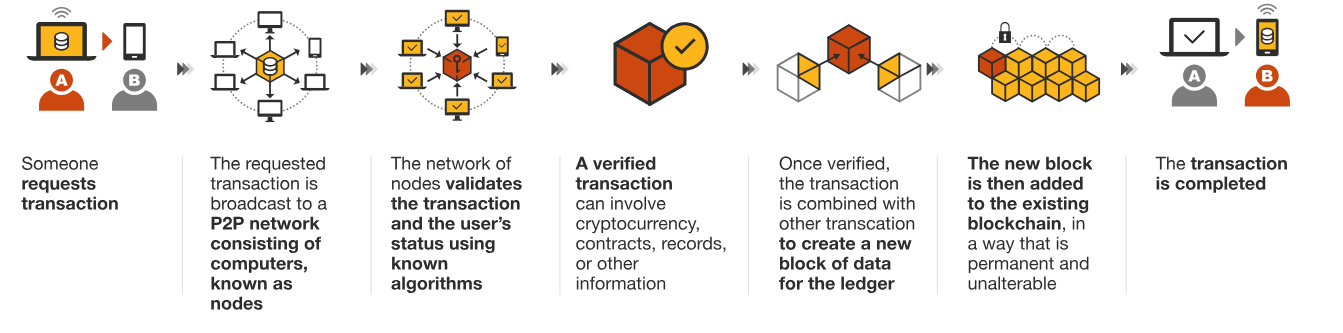
\includegraphics[width=0.8\textwidth]{images/blockcahin_how.png}
    \caption{How blockchain works \cite{pwcBlockchain}}
    \label{fig:pwc-blockchain}
\end{figure}

In payment systems, blockchain data contains the transactions of users. Transactions are stored in blocks, and each block is linked to the previous block by hashing its contents. In that way, a chain of blocks is created \autoref{fig:blockchain-blocks}.

\begin{figure}
    \centering
    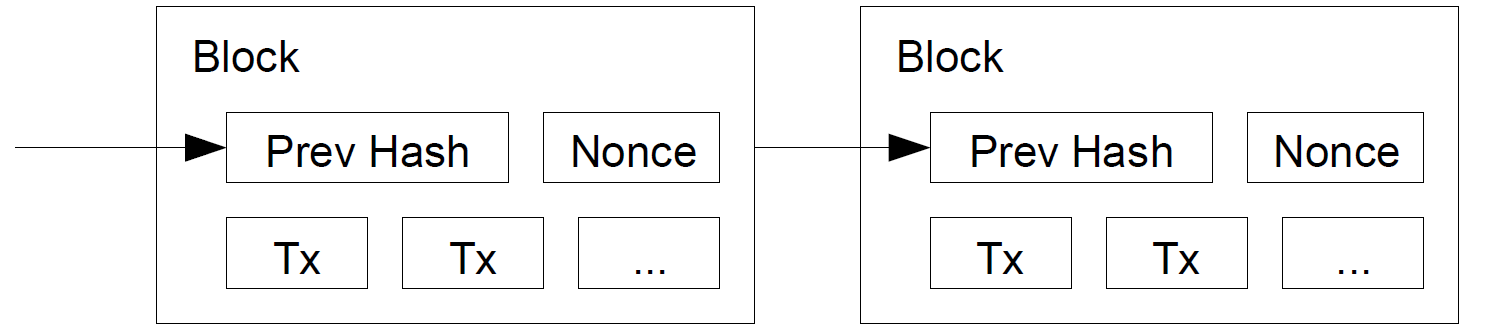
\includegraphics[width=0.8\textwidth]{images/chain_of_blocks.png}
    \caption{Blocks in Blockchain \cite{nakamoto2009bitcoin}}
    \label{fig:blockchain-blocks}
\end{figure}

\subsubsection{Permissioned vs Permissionless}
The consensus mechanism ensures that all participants agree on the same ledger. There are two categories of Blockchain, depending on whether those involved are known or not known to the system. 
\begin{itemize}
    \item \textbf{Permissioned}: Permissioned blockchains are private networks where access to the blockchain is restricted. In this type only authorized participants can join the network. This ensures that all participants are known and trusted.
    \item \textbf{Permissionless}: In a permissionless setting, anyone can join the network, participate in the consensus process, and view all transactions on the blockchain. However, in a permissionless blockchain, a mechanism to prevent sybil identities is required to ensure the validity of the consensus algorithm, such us Proof of Work (PoW) or Proof of Stake (PoS).
\end{itemize}

\subsubsection{How to track ownership in Blockchain}
In blockchains, there are basically two ways to do ownership tracking:
\begin{itemize}
    \item \textbf{UTXO model}: In UTXO (Unspent Transaction Output) model transactions contains inputs and outputs. Transaction inputs are references to previous unspent transaction outputs, meaning that they are constructed from a transaction but have not been used as inputs in any previous transaction. Each transaction consumes its transaction inputs and generates new UTXOs, specifying the amount of the cryptocurrency and the recipient address. participants need to maintain all unspent transactions and balance  is the sum of UTXOs destined to specific address.
    
    \item \textbf{Account-based model}: In the account-based model, each address has an account on the blockchain associated with a balance that is updated based on the currency transfer transactions that account issues or receives.

\end{itemize}
        % \section{Bitcoin}
    
    \chapter{Privacy in Payment Systems}
        \section{Privacy}

% //TODO: Write why he need privacy
Privacy is a very useful and beneficial feature in payment systems. First and foremost, payment activities involve some sensitive personal information. Users usually do not want this information to be disclosed in order to protect their personal information, as it can be used to discriminate against individuals based on their financial history or purchasing habits. 

Apart from the protection of personal data, the lack of privacy raises concerns in other areas as well ~\cite{SoKPrivacyPreservingComputing}.
It also has a negative impact on fairness by enabling front-running attacks ~\cite{FronRrunningAttacks}. In these attacks, a malicious individual monitors the transactions of other users and races to issue his own transaction, aiming to have it confirmed first. An example could be racing to win an auction by exploiting this advantage. It can also create "tainted" currency. That is, coins that no one wants to own because they are associated with an undesirable coin history, such as being part of an illegal trade.

The first level of privacy used by Bitcoin and most existing cryptocurrencies is pseudonymity. In this approach, transactions hide neither the participants nor the values transferred. Privacy relies on pseudonymous addressing, which aims to break the link between the addresses of the system and the identities of real users. Payment systems that use the permissionless setting allow and encourage users to have more than one such pseudonym. However, even this provides a very weak anonymity guarantee. Various de-anonymization attacks have been proposed in the literature ~\cite{meiklejohn2013fistful}, ~\cite{reid2013analysis}, ~\cite{ron2013quantitative}, ~\cite{tschorsch2016bitcoin}, based on clustering by analyzing either the inputs and outputs of the transactions or the behavior of the users ~\cite{SoKAnonymityInCryptocurrencies}.

Stronger privacy guarantees include the following properties: confidentiality and anonymity. Confidentiality hides the transaction amounts, while anonymity hides the pseudonyms of the real participants in a transaction. There are two levels of anonymity, set anonymity and full anonymity. In set anonymity, the user's identity is either one of $n$ possible identities, where $n$ is the size of the set. Full anonymity is provided when the participants can be any user of the system.

\begin{figure}
    \centering
    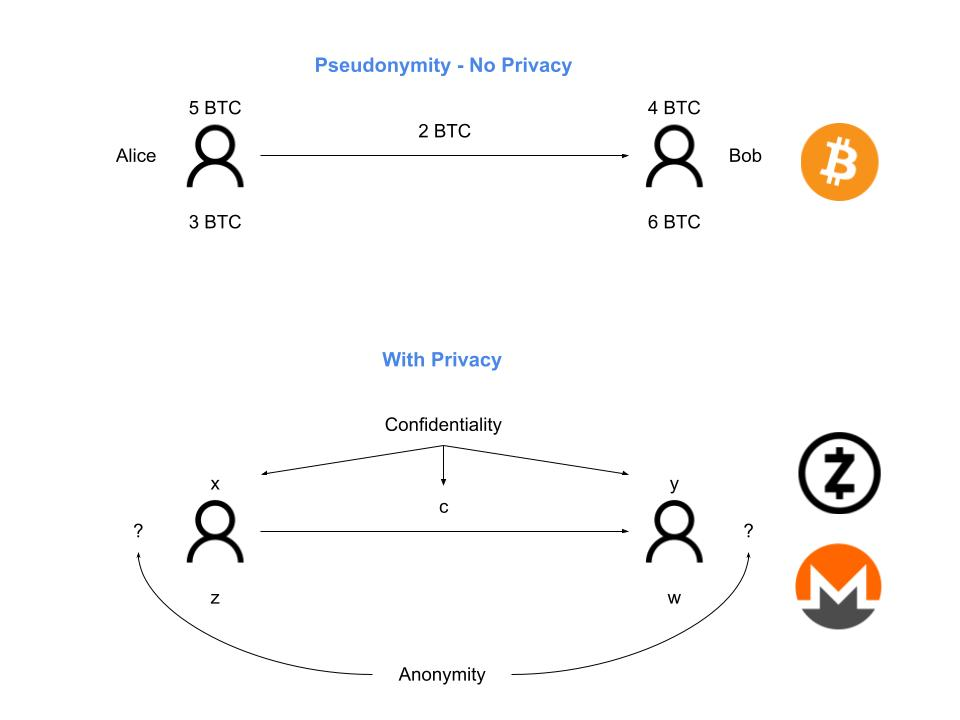
\includegraphics[width=0.9\textwidth]{images/privacy/Anonymity in blockchain.jpg}
    \caption{Privacy in Payment Systems}
    \label{fig:privacy_img}
\end{figure}

% The basic idea behind implement privacy in the payment systems are the following:
% \begin{itemize}
%     \item Hide transaction values inside
%         \textbf{commitments} (confidentiality).
%         \item Use \textbf{Anonymity Set} to disguise the real participants in the tx (anonymity).
%         \item Provide \textbf{ZK-Proofs} for the validity of tx.
% \end{itemize}

To implement privacy properties, private payment systems use the following basic idea: 
\begin{itemize}
    \item confidentiality is achieved through homomorphic commitments, which aim to hide the amounts transacted as well as the values of users' accounts. 
    % if an account-based scheme is used, 
    \item Anonymity is achieved through anonymity sets (e.g., shielded pools, ring signatures) that hide the pseudonyms of the real participants in a transaction.
\end{itemize} 
In addition, a necessary tool for private payment systems is zero-knowledge proof, which aims to ensure the validity of transactions without revealing the above information.
        \section{Private Schemes}
Some typical examples of private payment schemes (Zerocash \cite{Zerocash}, Monero \cite{Monero} and Quisquis \cite{fauzi2019quisquis}) are presented below:
% \subsection{Tumblers}
\subsection{Zcash}

Zerocash \cite{Zerocash} is a novel proposal for a cryptographic protocol that addresses the inherent privacy limitations of bitcoin. It introduces the concept of decentralized anonymous payment (DAP) scheme, meaning a digital currency system where all transactions are guaranteed to be completely anonymous. That is, the origin, destination, and amount are all hidden from the public ledger.

Zerocash achieves privacy through the use of Zero-Knowledge Succinct, Non-interactive Arguments of Knowledge (zk-SNARKs). This cryptographic tool is essential to prove that transactions are valid, without revealing any information about the parties involved in a transaction and the amounts involved. 

More specifically, Zerocash functions on top of any ledger-based currency (e.g. Bitcoin). First, each user generates an arbitrary number of address key pairs. These contain a public key $\pk$ that allows others to send payments to the user, and a secret key $\sk$ that is used to receive payments sent to the corresponding public key. Then Zerocash gives the ability to users to convert  regular coins into anonymous coins through the mint functionality. Afterwards, users can spend (move) this coins in transactions without revealing any information. 

\subsubsection{Mint coins}
When minting a coin, a user generates a secret trapdoor $\rho$, used to create a random serial number unique for each coin (through a PRF) and two randomnesses $r, s$. Then they create a commitment to the value of the coin, the recipient's address and the serial number in the two following steps. First, user computes an intermediate commitment $k$ using randomness $r$ for the concatenation of the recipient address and the trapdoor $\rho$, $k = \com(\pk||\rho ; r)$. In the second step user creates a commitment using randomness $s$ for the concatenation of the coin's value and the intermediate commitment $k$, $cm = \com(\v||k;s)$.
Finally the user publish on the blockchain the mint transaction $\txn_{MINT} = (\v, k, s, cm)$. 

Anyone can verify that $cm$ is a commitment to a coin of value $v$ by checking whether $\com(\v||k;s)$ is equal to $cm$. However, they will not be able to distinguish between the owner $\pk$ and the serial number, since these values are hidden inside the commitment $k$.

All of the minted coins are stored in a "shielded pool" and are not deleted when spend in order to provide anonymity.

\subsubsection{Pour coins (Spend functionality)}

In order to spend a coin anonymously, the user produces a zero-knowledge proof (using zk-SNARK) for the statement:
"I know the one opening ($\rho, r)$ of a coin commitment of the "shielded pool" and the corresponding secret key $\sk$ such that $k = \com(\pk||\rho ; r)$ and $sn = PRF(\sk, \rho)$.

After that user reveal the serial number $sn$. The serial number is used in order to handle double spending. Zerocash allocates a unique sequence number to each coin, which is published on-chain when the coin is spent. Therefore, an attempt at double spending is indicated by a new transaction that produces a sequence number(s) that has already been published.

Finally, user creates a new coin for the new recipient address with a new serial number.

After confirming and recording the pour transaction in the ledger, the new coins can be used for future transactions. Throughout this process, the use of zk-SNARKs and commitments guarantees that all details of the transaction, including the coin spent and the recipient of the new coin, remain private and secure. This process maintains user anonymity while preserving the integrity and validity of transactions within the Zerocash system.

\subsubsection{Merkle Tree}
As mentioned above, to ensure anonymity, no one can tell which coin was used in each transaction. 
Thus, the spent coins cannot be removed from the "shielded pool". As a result, its size increases with each transaction. Therefore, the naive approach to implement it as a list of coin commitments will lead to a linear growth for the blockchain size. 

A more efficient implementation is the use of Merkle trees. 
Zerocash maintains an efficiently updateable Merkle tree over the growing coin commitment list \autoref{fig:zcash-merkle}. As a result, the space complexity is reduced to logarithmic.

\begin{figure}
    \centering
    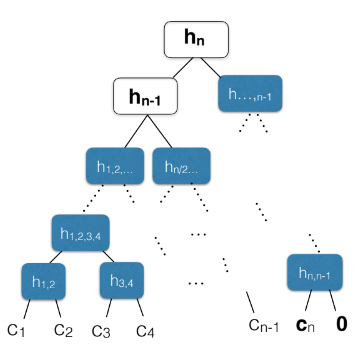
\includegraphics[width=0.8\textwidth]{images/zcash/merkle tree.png}
    \caption{Zerocash Merkle Tree of Coin Commitments}
    \label{fig:zcash-merkle}
\end{figure}


\subsection{Monero}

Monero \cite{Monero} is also a privacy-focused cryptocurrency that provides both anonymity and confidentiality. It uses a different approach than Zerocash. Instead of zk-SNARKs, Monero achieves its privacy through the use of ring signatures, stealth addresses, and ring confidential transactions. 
Ring signatures and stealth addresses provide anonymity and are described in more detail below.
Ring confidential transactions provide confidentiality by using pedersen commitments to hide the amount and zero-knowledge proof to ensure the validity.

Users in Monero also own a key-pair of a public and a secret key, while its work model is the UTXO model same as in Bitcoin.

\subsubsection{Ring signatures}
Monero users the ring signatures \cite{Rivest2006} to hide the sender of the transaction, as well as the transaction graph \autoref{fig:ring-sig-ex}. A ring signature is a cryptographic technique that allows a member of a group to anonymously sign a message on behalf of the group, while hiding the identity of the person signing the message. In other words, this primitive allows users to specify a set of possible signers without revealing which member actually created the signature.

In order to create such a signature the signer executes the following steps. First, they choose a set of public keys, including his own, called a 'ring'. Then, they use their own private key to create a signature for the message. However, they combine it with the public keys of others in the ring rather than signing directly with their private key., in order to hide the real signer.

Anyone can publicly verify that the signer is a member of the ring by using the public keys of the ring. However they cannot distinguish which corresponding secret key was used to produce the signature.

So in Monero, when a user wants to create a transaction, he chooses an anonymity set that includes the public keys of other users' utxo inputs, and creates a ring signature with their own utxo input (corresponding to their public address) and those in the anonymity set.
Since no one can distinguish the utxo input that was spent in the transaction, it cannot be removed from the utxo set either.

\begin{figure}[!tbp]
    \begin{subfigure}[b]{0.5\textwidth}
        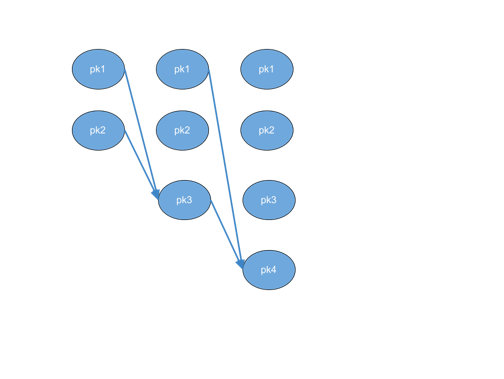
\includegraphics[width=\textwidth]{images/monero/ring_sing_ex.png}
        \caption{}
        \label{fig:f1}
    \end{subfigure}
    \begin{subfigure}[b]{0.5\textwidth}
        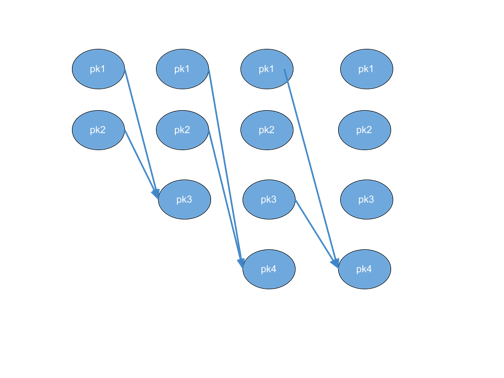
\includegraphics[width=\textwidth]{images/monero/ring_sing__bad_ex.png}
        \caption{}
        \label{fig:f2}
    \end{subfigure}
    \caption{Ring signature example. \autoref{fig:f1} Either one of $\pk_1, \pk_2$ sends to $\pk_3$, so none of them can be removed from utxo. \autoref{fig:f2} There are cases where anonymity is not guaranteed. Both $\pk_1, \pk_2$ is spent after second transaction, so $\pk_3$ is the sender of the third transaction.}
    \label{fig:ring-sig-ex}
\end{figure}

\subsubsection{Stealth addresses}

In order to improve its anonymity, each Monero transaction generates a one-time destination address, known as a stealth address. This address is derived from the recipient's public key, but is unique for each transaction, ensuring that the recipient's public address remains private.

An example of such addresses is presented bellow implemented using elliptic curves:

Let Alice be the sender and Bob the receiver. Bob owns a key-pair of the form $\pk = (A,B), \sk = (a,b)$ such that $A = aG, B= bG$ where $G$ is the base of the used elliptic curve. Then Alice generates a random $r$ and calculates $P = H{rA}G + B$, where $H$ is a collision-resistant hash function. Alice publish $P, R = rG$ together with the transaction. Afterwards, Bob can check if $P^\prime = H{aR}G + B$. If the transaction is destined for Bob then it holds that $P^\prime = P$.

Obviously, no one will know that this address is intended for Bob, but only Bob can prove that this address is associated with him. In this way, Monero hides the recipient address of the transaction.

% \subsubsection{Ring Confidential Transactions} 
\subsection{Quisquis}
\subsection{Comparison}

Among the three private systems mentioned above, Zerocash offers full anonymity, while the other two offer set anonymity. However, both Zerocash and Monero suffer from a very important limitation. That is the size of storage cost that each miner should maintain in the system. Since a UTXO input is not identified when spent (to preserve anonymity) these two system have a growing list of UTXOs. This fact prevents miners from storing a concise version of the blockchain. Updatable Public Keys primitive, that Quisquis uses, offer a solution to this problem. As a result, Quisquis manage to maintain a constant storage cost with respect to the number of transactions.

    \chapter{Auditability in Private Payment Systems}
    % \section{Auditability in Private Payment Systems}

Auditability plays a pivotal role in ensuring the integrity, transparency, and regulatory compliance of payment systems. 
In financial transactions, where trust and security are paramount, regulatory functions serve as critical safeguards to protect against fraud, money laundering, and other illicit activities.
These regulatory functions that appear in the literature can be categorized in transaction and user level.\\
On the transaction level regulatory functions can include data such as: 
\emph{value limits} (e.g. a threshold in the transfer amount), 
\emph{tracing tags}, that provide links between transactions,
\emph{revealing the transaction value and/or participants},
\emph{tax rate}, deducting a transaction's value portion towards a pre-determined account.\\
On the user level regulatory functions can include:
\emph{information of user's sum of values} (e.g. total amount of funds received/spent in a specific period of time),
\emph{user revocation}, meaning that specific policies are applied only to users in a "blacklist",
\emph{deriving statistical information} (e.g. learning th average transacted value in a time from user's past transactions),
\emph{revoking a non compliant user's anonymity}.

There are two approaches in order these regulation to be enforced, \emph{auditability} and \emph{accountability}.
On the one hand, auditability refers to a protocol where an external auditor can learn the requested information through the data that are stored on the blockchain.
This protocol could be either interactive with the users, meaning their consent is required, or non-interactive.
On the other hand, accountability refers to recurrently execution of policies by system fucntionalities when certain predicate is satisfies.
In other words, transactions that does not comply with system's policies will never be verified and stored in the blockchain.
Therefore, there is no need of active participation of an external auditor, since the policies are enforced during the verification phase of the transaction. 

Afterwards, an overview of existing distributed payment systems which combines both privacy and auditability is presented.
Following the structure of \cite{SokAuditability} these systems are divided into two categories depending on the power given to the auditors from the disclosed information:
There are systems that requires a centralized trusted desingated athority to perform the regulation functions and the systems that does not assume any explicit auditor.

    \section{Centralized Authority}

A common way to implement auditability in private systems is to introduce a centralized authority or group of authorities (multi-party computation). Such authority can either be an external designated auditor or can enforce the internal policy rules in each transaction (accountability). 

According to this approach users embed auxiliary information to the transactions that are encrypted under the public key of a designated trusted auditor (\autoref{fig:cent-aud}). Therefore, the users data are remain private for the rest of the system's participants except the centralized authority, which can decrypt the auxiliary information at any point without the consent of the users. 

\begin{figure}
    \centering
    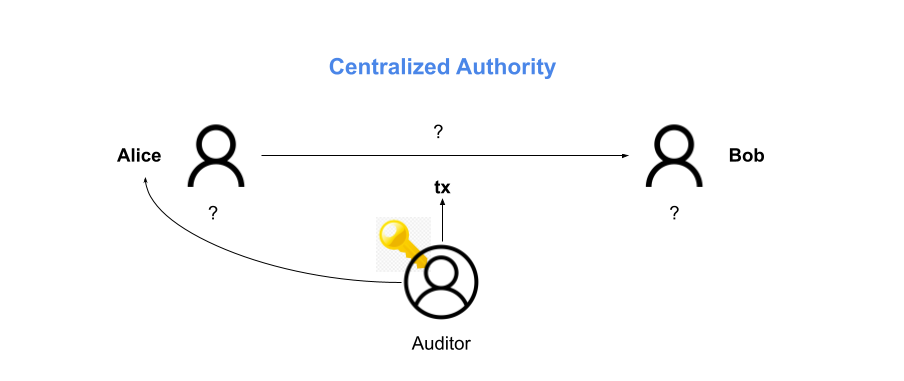
\includegraphics[width=0.9\textwidth]{images/privacy/Auditability in blockchain - Centralized.png}
    \caption{Auditability - Centralized Authority}
    \label{fig:cent-aud}
\end{figure}


This method can be a trivial solution for adding auditability to privacy-preserving systems. However, all the data is collected by a single centralized authority, which accumulates excessive power. This fact can negatively impact the user privacy.

One example that implement this approach is presented below:

\subsection{Zcash extension}
% \subsection{PRCash}
% \subsection{ACCDET}


\section{General Auditor}

In order to avoid gathering all the information to one (or a group) centralized authority a second approach were proposed. That is an interactive protocol between the user being audited and the auditor. In this case, the auditor, who can be \textit{any} auditing authority, can ask specified questions which derives from system's policies. Users answer to this questions with zero-knowledge proofs based on data that are stored on chain (\autoref{fig:gen-aud}).

This protocol implies the concent and the cooperation from the audited user. However, this requirement cannot be exploited by non-compliant users due to the fact that refusal to cooperate with authorities can be considered equivalent to a failed audit.

\begin{figure}
    \centering
    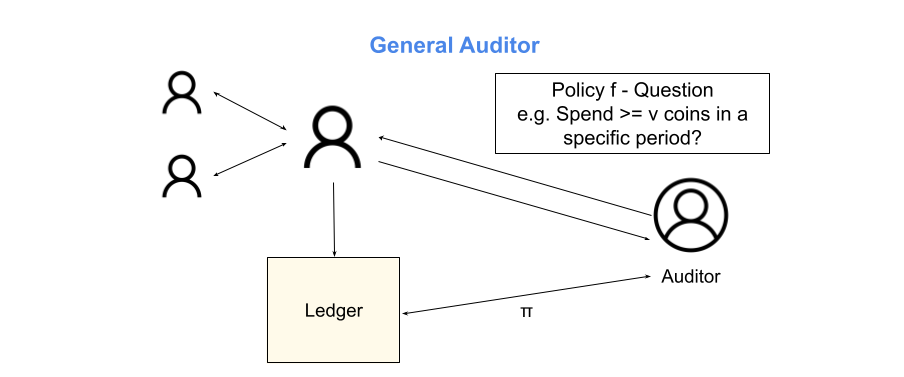
\includegraphics[width=0.9\textwidth]{images/privacy/Auditability in blockchain - General Auditor.png}
    \caption{Auditability - General Auditor}
    \label{fig:gen-aud}
\end{figure}

Some typical examples of auditable private decentralized systems who implement a general auditor are presented below:

\subsection{zkLedger}
% \subsection{miniLedger}
\subsection{PGC}

    \chapter{AQQUA: Augmenting Quisquis with Auditability}
        \section{Overview}

\subsubsection{Objective}
The proposed solutions in the literature that aim to combine privacy and auditability using a general auditor and not a centralized authority suffer either from limited scalability or does not provide full privacy.

Therefore, we aim to construct an efficient, anonymous, confidential and auditable system that can also support concurrent transactions and maintain a stable state size regardless the number of the user or the transaction history. In order to create such a system we propose AQQUA which augments the Quisquis \cite{fauzi2019quisquis} DPS system by adding a general auditor. Therefore, AQQUA combines the anonymity of Quisquis with the policy expressiveness and regulation of PGC \cite{PGC}. That is, the auditor can execute queries about the upper bound on amount the user sent/received in a period of time, non-participation of a user in a specific transaction or period of time, as well as the exact value sent/received in a transaction.

We chose to augment Quisquis, since, as it is already mentioned, it is a fully private system, offering both anonymity and confidentiality, while it has a constant storage cost with respect to the number of transactions. In addition, due to the fact that the anonymity set that uses in order to hide the participants of a transaction does not include all the users of the system, as in zkLedger, Quisquis can support concurrent transactions. 

\subsubsection{Challenges}
Designing AQQUA required to overcome the following key challenge, enabling auditing functionalities while still users preserve their privacy. Because of the anonymity property, user can hide their accounts and as a consequence the necessary amounts for the auditing procedure. In addition, since Quisquis is permissionless and private, an authority cannot enforce some effective penalties for non-compliant users. 

To overcome this challenge, we introduce a registration functionality to Quisquis through a Registration Authority. That is, users must first register to the systems and provide their real-world credentials. Afterward, they can create new unlinkable accounts that will be used in order to transact within the system. The registration functionality provides a way for the system to know the users that utilize the system as well as to penalize them outside of the system scope. In addition, AQQUA splits the state into two sets. It keeps the UTXO set used in Quisquis that contains the unspent accounts of the user, but also adds a new set that contains the public registration information of users along with necessary information in order to ensure that users cannot hide information during the audit procedure.
        \section{Preliminaries}
        % //TODO I think that notation should apply to basic stuff and not system related.
\subsection{Notation}
% TODO: add explanation for 'acct.pk' (when we have a tuple, a=(b, c, ...) we denote a.b = b)
We denote by $\secpar$ the security parameter. 
We denote by $\msgspace$ the message space and by $\randspace$ the randomness space of our cryptographic schemes.
$\vset = \{0,\dots,V\}$ is the set that defines the range of valid currency values, where $V$ is an upper bound on the maximum possible number of coins in the system ($|\vset| \ll |\msgspace|$). 
When an element $x$ is sampled uniformly at random from a set $\mathcal{X}$, we write $x \sample \mathcal{X}$.
Given a tuple $t = (a,b)$ we refer to its parts using the dot notation, i.e. $t.a$ or $t.b$.
We  denote $(a^x,b^x)$ as $t^x = (a,b)^x$.
% We denote the initial public key with which the user has initially registered in the system as $\inpk$, the current public key of a user's account $\acct$ as $\pk$ and the output public key of update algorithms as $\pk'$.
% Also, the secret key of the user as $\sk$. 
% We use $n$ to denote the number of users that belong to an anonymity set $\anset$ and the participants of the transactions as $\pset$ 
% //TODO is n fixed?
% The $\numaccs$ states the number of accounts are related to a specific user.
% A commitment to a value $v$ is denoted by $\comm{v}$. 



        \subsection{Commitments}
We use a commitment scheme $\commit$ relative to a public key $\pk$ that, given a message $m \in \msgspace$ and randomness $r \in \randspace$,
computes $\comm{m} \gets \commit(\pk, m;r)$. 
Our commitments must satisfy the following properties: 
\begin{itemize}
    \item \textbf{Computational hiding}: An adversary has negligible advantage in distinguishing between $\commit(\pk, m_0;r_0)$ 
    and $\commit(\pk, m_1;r_1)$, where $r_0, r_1 \sample \randspace$.
    \item \textbf{Unconditional binding}: A commitment cannot be opened to two different messages, even with the knowledge of the secret key $\sk$.
    \item \textbf{Additively homomorphic}: For given operation $\odot$ it holds that \\
     $\commit(\pk, m;r) \odot \commit(\pk, m';r') = \commit(\pk, m+m';r+r')$.
    \item \textbf{Key-anonymity}: An adversary cannot distinguish between \\
     $(m, \pk_0, \pk_1, \commit(\pk_0, m))$ and $(m, \pk_0, \pk_1, \commit(\pk_1, m))$ for any honestly generated public keys $\pk_0, \pk_1$ and adversarially chosen message $m$.
\end{itemize}

We construct such a scheme using the unconditionally binding commitments of~\cite{fauzi2019quisquis}. They are defined in a prime-order $p$ group $(\group, g, p)$ generated by $g$, where the $\ddh$ problem is hard.
In essence, ElGamal `encryption' is used in the exponent where the public keys are of the form $\pk = (g, h) \in \group^2$. 
Specifically,  
 $\commit(\pk, m; r)$ yields $\comm{m} = (c, d)$, where $c = g_i^r$ and $d = g^m h_i^r$.

 Using UKPs as the commitment public keys, one can verify and open commitments using the secret key, without needing to know the randomness used.
\begin{itemize}
    \item $\verifycom(\sk, \pk, \com, m)$: Checks if $\com = (c,d)$ is a commitment to $m$ under $\pk$, by checking if $ d = g^m c^\sk $ holds.
    % \item $\verifycom(\pk, \com, m, r)$: Checks if $\com = (c,d)$ is a commitment to $m$ under $\pk$ with randomness $r$, by checking if $c = g^r$ and $d = g^m h^r$.
    \item $\opencom(\sk, \comm{m})$: Given $\comm{m} = (c, d)$, calculates $m$ by calculating $dc^{-\sk}$ and brute-forcing to obtain $m$.
\end{itemize}
        \section{Definition of an Auditable Private Decentralized Payment System}
        We now describe the components of an auditable and private DPS like AQQUA:

        \subsection{Entities}
\begin{itemize}
    % [1. Why we need users to register
%   need to connect user pk in the system with real user identity (in order to potentially penalize non-compliant users)]-> intro or registration authority (with the citation)
    \item \emph{Registration Authority} (\RA): The role of the $\RA$ is to enroll new users into the system. Users register by sending their real-world identity information together with an initial public key that they create on their own.
    The $\RA$ stores this information off-chain. 
    All the accounts that transact on behalf of this real-world user will originate from this initial public key, through the mechanism of \autoref{UPK}.
    The purpose of the registration procedure is essential as it establishes a link between a user's public key and their real identity, to be used for the potential penalization of non-compliant users.
    
    \item \emph{Audit Authority} (\AA): 
    Its role is to initiate the audit procedure in order to verify that users comply with the system's policies. 
    If a user of the system is found to be non-compliant, the $\AA$ will collaborate with the $\RA$ to enforce the relative penalties.

    \item \emph{Users} (\UU): Users of the system that transact with each other.
\end{itemize}
    
        \subsection{State}
In AQQUA, the state (denoted $\state$) consists of the following two sets:
\begin{itemize}
\item $\utxoset$: A table containing the `unspent' accounts, i.e. the accounts that are recorded as outputs of a valid transaction, but 
have not (yet) been used as inputs.% in any newer transaction.
\item $\usersset$: A table containing one tuple for each physical user, which is composed of the user's initial public key and a commitment to the number of accounts owned by the user.
%  A table containing tuples composed of users' initial public keys and commitments to information necessary to perform auditing.
% A table containing records of the form  $\userinfo=(\inpk,\comm{\numaccs})$, where $\inpk$ represents the initial public keys of the user, and $\comm{\numaccs}$ is a commitment to the number of accounts controlled by the user in the $\utxoset$.
\end{itemize}
        \subsection{Accounts}
User accounts are of the form $\acct = (\pk,\comm{\varbl}, \comm{\varout}, \comm{\varin})$, where $\varbl$ is the account balance and $\varout, \varin$ is the total amount that the account has sent and received, respectively.
Each user may own multiple accounts which are stored in the $\utxoset$. 
The following functionalities create, verify and update accounts.

\begin{itemize}
    % //TODO: 0 here (in a box) or bl?
    \item $\acct \gets \newacc(\inpk; r_1, r_2, r_3, r_4)$: takes as input a public key $\inpk$ and outputs a new account of the form $\acct = (\pk, \comm{\varbl}, \comm{\varout}, \comm{\varin})$, where $ \pk = \upd(\inpk; r_1), \comm{\varbl} = \commit(\pk, 0;r_2),  \comm{\varout} = \commit(\pk, 0;r_3)$ and $\comm{\varin} = \commit(\pk, 0;r_4)$.
    % \item $\acct \gets \newacc(\inpk, \varbl; r_1, r_2, r_3, r_4)$: takes as input a public key $\inpk$ and outputs a new account of the form $\acct = (\pk, \comm{\varbl}, \comm{\varin}, \comm{\varout})$, where $ \pk = \upd(\inpk; r_1), \comm{\varbl} = \commit(\pk, \varbl;r_2),  \comm{\varout} = \commit(\pk, 0;r_3)$ and  \\
    % $\comm{\varin} = \commit(\pk, 0;r_4)$

    % //TODO: do we need to verify upk?
    \item $0/1 \gets \veract(\acct,\sk,\varbl,\varout,\varin)$: Parses $\acct$  as $(\pk, \com_1, \com_2, \com_3)$ and outputs 1 if
    \begin{align*}
        & \vercom(\sk, \pk, \com_1, \varbl) \land \vercom(\sk, \pk, \com_2, \varout) \land \\
        & \vercom(\sk, \pk, \com_3, \varin) \land (\varbl, \varout, \varin \in \vset)
    \end{align*}

    \item $\{\acct'_i\}_{i=1}^n \gets \updacc(\{ \acct_i, {\vbl}_i, {\vin}_i, {\vout}_i \}_{i=1}^n; r_1,r_2,r_3,r_4)$ takes as input a set of accounts $\acct_i = (\pk_i, {\com_{\varbl}}_i, {\com_{\varout}}_i, {\com_{\varin}}_i)$ and values
    ${\vbl}_i, {\vout}_i, {\vin}_i \in \vset$ and outputs a new set of accounts  $\{\acct'_i\}_{i=1}^n$,
    where 
    \begin{align*}
        \acct'_i \gets  &(\upd (\pk;r_1), {\com_{\varbl}}_i \ \odot \commit(\pk, {\vbl}_i;r_2), \\
                        & {\com_{\varout}}_i \ \odot  \commit(\pk,{\vout}_i;r_3 ), {\com_{\varin}}_i \ \odot  \commit(\pk, {\vin}_i;r_4)).
    \end{align*}

    % \item $\{\acct'_i\}_{i=1}^n \gets \updacc(\{ \acct_i, {\vbl}_i, {\vin}_i, {\vout}_i \}_{i=1}^n; r_1,r_2,r_3,r_4)$ takes as input a set of accounts $\acct_i = (\pk_i, \comm{\varbl_i}, \comm{\varout_i}, \comm{\varin_i})$ and values \\
    % ${\vbl}_i, {\vout}_i, {\vin}_i \in \vset$ and outputs a new set of accounts  $\{\acct'_i\}_{i=1}^n$,
    % where 
    % \begin{align*}
    %     \acct'_i \gets  &(\upd (\pk;r_1), \comm{\varbl_i} \ \odot \commit_\pk({\vbl}_i;r_2), \\
    %                     & \comm{\varout_i} \ \odot  \commit_\pk({\vout}_i;r_3 ), \comm{\varin_i} \ \odot  \commit_\pk({\vin}_i;r_4)).
    % \end{align*}

    \item $0/1 \gets \verupdacc(\{\acct_i^\prime, \acct_i, {\vbl}_i, {\vout}_i, {\vin}_i\}_{i=1}^n; r_1,r_2,r_3,r_4)$: outputs 1 if
    \begin{align*}
        \{\acct_i^\prime\}_{i=1}^n =  \updacc(\{\acct_i, {\vbl}_i, {\vout}_i, {\vin}_i\}_{i=1}^n; r_1,r_2,r_3,r_4)  \land 
                                      (|\vbl|,\vout, \vin  \in \vset).
    \end{align*}

\end{itemize}
        \subsection{User information}
Each real-world user is associated with a tuple $\userinfo=(\inpk,\comm{\numaccs})$, stored in the $\usersset$.
The public key $\inpk$ is an initial public key provided at the time of registration. 
The public key of every account owned by the user will share the same secret key with $\inpk$.

The value $\numaccs$ is the number of accounts in the $\utxoset$ that are owned by the user, and is stored as a commitment so that it remains hidden. 
Keeping track of the number of accounts a user owns is necessary in order to support  policies related to value limits, such as the total amount a user has received or sent in a period of time. Otherwise, such policies could be easily bypassed through the creation of sybil identities~\cite{SokAuditability}.
 The opening of the commitment $\comm{\numaccs}$ will be revealed only to the $\AA$ during the auditing procedure.

The following functions create, verify and update $\userinfo$ entries of the $\usersset$.

\begin{itemize}
    % TODO: Add comment to explain where the initial balance comes from
    \item $(\sk, \userinfo, \acct) \gets \genuser()$: Picks $r_1, r_2, r_3, r_4, r_5 \sample \randspace$ and let $\vec{r} = (r_1, r_2, r_3, r_4)$. Then runs $(\sk, \inpk)\gets \kgen()$, $\acct \gets \newacc(\inpk; \vec{r})$, calculates the tuple $\userinfo = (\inpk, \commit(\inpk, 1;r_5))$  and returns
    $(\sk, \userinfo, \acct)$.
    % \item $(\sk, \userinfo, \acct) \gets \genuser(\varbl)$: Picks $r_1, r_2, r_3, r_4, r_5 \sample \randspace$ and let $\vec{r} = (r_1, r_2, r_3, r_4)$. Then runs $(\sk, \inpk)\gets \kgen()$, $\acct \gets \newacc(\inpk, \varbl; \vec{r})$ and returns
    % \begin{equation*}
    %     (\sk, \userinfo = (\inpk, \commit_{\inpk}(1;r_5)), \acct)
    % \end{equation*}
    
    \item  $0/1 \gets \veruser((\inpk, \com), (\sk, \numaccs))$: outputs 1  if \\ 
   $
        \vercom(\sk, \inpk, \com, \numaccs)
        \land (\numaccs \in \vset)
    $

    % //TODO: fix indexing (for i)- is it pk_0_i (index on 0) or (pk_0)_i so i is next to pk_0?
    \item $\{\userinfo'_i\}_{i=1}^n \gets \upduser(\{\userinfo_i, {\vnumaccs}_i\}_{i=1}^n; r)$ takes as input a set of user-value pairs where $\userinfo_i = (\pk_{0_i},\com_{\numaccs i})$ and ${\vnumaccs}_i \in \vset$ and outputs a new set of users $\{\userinfo'_{i}\}_{i=1}^n = \{(\pk_{0_i}, \com_{\numaccs i}^\prime)\}_{i=1}^n$ 
    where 
    \begin{equation*}
        \com_{\numaccs i}^\prime = \com_{\numaccs i} \odot \commit(\inpk, \vnumaccs;r)
    \end{equation*}

    \item $0/1 \gets \verupduser(\{\userinfo'_i, \user_i, {\vnumaccs}_i\}_{i=1}^n; r)$ outputs 1 if
    \begin{equation*}
        \{\userinfo'\}_{i=1}^n = \upduser(\{\userinfo_i, {\vnumaccs}_i\}_{i=1}^n; r) \land (\vnumaccs \in \vset)
    \end{equation*}
\end{itemize}
        \subsection{Policies}
\label{ssec:Policies}
% // TODO: fix alignment!!
An auditable DPS should support a rich set of compliance policies.
They can be captured as predicates over an initial public key $\inpk$, a time period represented by a starting state $\state_1$ and an ending state $\state_2$, and auxiliary information $\aux$ which is dependent on an specific compliance goal. In all the policy predicates, we use the notation $A_1, A_2$ to denote the set of accounts in $\snap_1.\utxoset, \snap_2.\utxoset$ that are owned by the owner of $\inpk$.

\begin{itemize}
    \item Sending limit policy $f_{\sendlimit}$: The total amount a real-world user can send within a specific period. It can be determined by the $\AA$ off-chain and announced to the user for a specific period, depending on the application. The $\snap_1, \snap_2$ are the states of the blockchain at the beginning and end of the period, respectively.
    % // TODO: write somewhere that this can be used for anti-money laundering, i.e. "i know that someone sent 100k to fund some activity, prove to me that you are not them.
    \begin{align*}
        f_{\sendlimit}(\inpk, (\snap_1, \snap_2), \srlimit) = 1 \iff 
        \left\{ \begin{aligned}
                            &  \left(\sum_{\acct\in A_2}{\varout} - \sum_{\acct \in A_1}{\varout} \right)
                            \leq \srlimit 
                 \end{aligned} \right\}
    \end{align*}
    where $\varout$ is the opening of $\comm{\varout}$ of an account $\acct$, using the account's secret key $\sk$.
    \item Receiving Limit policy $f_{\receivelimit}$: Similarly, the total amount a `physical' user can receive from other accounts.
        \begin{align*}
           f_{\receivelimit}(\inpk, (\snap_1, \snap_2), \srlimit) = 1  \iff 
           \left\{ \begin{aligned} 
                    & \left(\sum_{\acct\in A_2}{\varin} - \sum_{\acct \in A_1}{\varin}\right) \leq \srlimit
            \end{aligned} \right\}
        \end{align*}
        where $\varin$ is the opening of $\comm{\varin}$ for account $\acct$, calculated using the account's secret key $\sk$.

        % ---- begin tax policy(removed) ----
        % \item Tax policy $f_{\rate}$: A portion $\rho$ of the transferred amount in a transaction is sent to the tax office, where $\rho$ is an application-dependent rate. We assume that $\rho=\alpha/\beta$, where $\alpha,\beta$ are two integers. Here, $\snap_1, \snap_2$ are the states before and after the user's transaction is applied, respectively.
        % % // TODO: write a description once we settle with tax.
        % % Each transaction is taxed at a predetermined rate $\rho$.
        % \begin{align*}
        %     f_{\rate}(\inpk, (\snap_1, \snap_2), \alpha, \beta) = 1 \iff 
        %     \left\{ \begin{aligned}  
        %         % & \forall \acct \in A_1\cup A_2, \verkp(\sk, \acct.\pk)=1 \land  \\
        %         % & \rho = \alpha / \beta \land \\
        %         % &  \frac{\sum_{\acct\in A_2}{\varin} - \sum_{\acct \in A_1}{\varin}}{\acct_{\taxoffice}^{A_2}.\varbl - \acct_{\taxoffice}^{A_1}.\varbl} = \frac{1}{\rho}
        %         & \alpha \cdot \left( \sum_{\acct\in A_2}{\varin} - \sum_{\acct \in A_1}{\varin} \right) = \\
        %          &\beta \cdot \left( \acct_{\taxoffice}^{A_2}.\varbl - \acct_{\taxoffice}^{A_1}.\varbl \right) 
        %     \end{aligned} \right\}
        % \end{align*}
        % where $\acct_{\taxoffice}$ the predetermined address of tax office.
        % ---- end tax policy(removed) ----
        % where $\varin$ is the opening of $\comm{\varin}$ of an account $\acct$ using the account's $\sk$ and $\vtof$ is a value send to the tax office.

        % If we want the tax policy to be between two txns
        % \begin{multline*}
        %     f_{\rate}(\sk, \txn, \rho) = 1 \iff \\
        %     \exists \acct_s \in \txn.\inputs, \verkp(\sk, \acct_s.\pk)=1 \land \\ 
        %     \exists \acct'_s \in \txn.\outputs, \verkp(\sk, \acct_s.\pk)=1 \land \\
        %     v = \acct_s.bl - \acct'_s.bl \in \vset \land \\
        %     \acct_{to} \in \txn.\inputs \land \acct'_{to} \in \txn.\outputs \land \\
        %     \frac{v}{\acct'_{to}.bl - \acct_{to}.bl} = \frac{1}{\rho},
        % \end{multline*}

        \item Open policy $f_{\open}$: The value of the amount sent or received by a user in a transaction.
        \begin{align*}
            f_{\open}(\inpk, (\snap_1, \snap_2), v_{\open}) = 1 \iff 
            \left\{ \begin{aligned}   
                % & \forall \acct \in A_1 \cup A_2, \verkp(\sk, \acct.\pk)=1 \land \\
                % //TODO: the parenthesis could be bigger- its (a or b) and c -that's why we need it!
            & (v = \left(\sum_{\acct \in A_{2}}\varbl - \sum_{\acct \in A_{1}}\varbl \right)\in \vset \\
            &\lor v = \left(\sum_{\acct \in A_{1}}\varbl - \sum_{\acct \in A_{2}}\varbl \right)\in \vset )\\
            & \land v = v_{\open} 
        \end{aligned} \right\}
        \end{align*}
        where $\varbl$ is the opening of $\comm{\varbl}$ of an $\acct$.

        \item Transaction Value Limit $f_{\txnlimit}$: Upper bound to the total transferred amount that can be sent in a transaction.
        \begin{align*}
            f_{\txnlimit}(\inpk, (\snap_1, \snap_2), v_{\max}) = 1 \iff  
            \left\{ \begin{aligned} 
            & v = \left(\sum_{\acct \in A_1}\varbl - \sum_{\acct \in A_2}\varbl \right) \leq v_{\max} 
            \end{aligned} \right\}
        \end{align*}
        
        \item Non-participation $f_{\nonpart}$: Non-participation in a specific transaction $\txn$ or inactivity of the user for a time period. The states $\snap_1, \snap_2$ are the states before and after a transaction is applied or at the beginning and end of the period.
        \begin{align*}
            f_{\nonpart}(\inpk, (\snap_1, \snap_2)) = 1 \iff  
            \left\{ 
                \begin{aligned} 
                    % \land & \left(\sum_{\acct \in A_{1}}\varbl - \sum_{\acct \in A_{2}}\varbl \right) = 0 \\
                    \land & \left(\sum_{\acct \in A_{1}}\varout - \sum_{\acct \in A_{2}}\varout \right) = 0 \\
                    \land &\left(\sum_{\acct \in A_{1}}\varin - \sum_{\acct \in A_{2}}\varin \right) = 0
                \end{aligned} 
            \right\}
        \end{align*}

        % TODO: do we want blacklist? can we just check if pk0 is in userset?
        % TODO: Remove blacklist predicated
        % \item Blacklist $f_{\blacklist}$: Exclusion from set of initial public key of users who are not compliant with the system's policies.
        % \begin{align*}
        %     f_{\blacklist}(\sk, \usersset, \blist) = 1 \iff 
        %     \left\{ \exists \inpk \in \usersset \smallsetminus \blist \land \verkp(\sk, \inpk) \right\}
        % \end{align*}
         
\end{itemize}

% These information needed for each policy $(\srlimit, \rho)$ is included in the corresponding algorithms implementing these policies in the $\aux$ variable.
        \subsection{Functionalities}
An auditable private decentralized payment system is a tuple of polynomial-time algorithms defined as below:

\begin{itemize}
    % \item $(\state) \gets \setup(\secpar, \vec{\varbl})$: 
    \item $(\instate, \params) \gets \setup(\secpar)$: 
    Generates the initial state of the system $\instate$ and the public parameters $\params$, which are implicitly given as input to all other algorithms.
    % It runs the $\genuser, \newacc$ algorithms and initializes the User and UTXO sets (to potentially empty sets). 

    \item $(\sk, \userinfo, \acct, \pi) \gets \reg()$: 
    Used by a user to create the registration information $\userinfo$ and their first account $\acct$.
    % \item $(\sk, \userinfo, \acct, \pi_m, \pi_a) \gets \reg(\varbl)$: 
    % Used by a user to create the registration information $\userinfo$ and an initial account $\acct$ with specified balance $\varbl$.
    % Used by a user to create the registration information, $(\inpk, \comm{\numaccs})$ a pseudonym within the system and a commitment to the number of accounts this pseudonym is associated with, as well as an initial account $\acct$ with specified balance $\varbl$.
    
    % Used by a user to create an initial public key $\inpk$ in order to use the system. Internally runs $(\sk, \userinfo = (\inpk, \comm{\numaccs})) \gets \genuser(\secpar)$ and creates a zk-proof $\pi$ that the number of the existing accounts in the UTXO set $\comm{\numaccs}$ is equal to 0. 

    \item $0/1 \gets \verreg(\userinfo, \acct, \pi, \state)$: 
        Used by the Registration Authority to verify the registration information and the account of a user.
    % \item $0/1 \gets \verreg(\userinfo, \acct, \pi_m, \pi_a, \state)$: 
    %     Used by the Registration Authority to verify the registration information and the created account of a user.
        % //TODO: do we want seperate verify register algorithms for the RA and the miners?

    \item $\state' \gets \applyreg(\userinfo, \acct, \state)$:
        Used by the Registration Authority to add a user to the system after their successful registration.
    
    \item $\txn = (\{\acct\}_{i=1}^n, \{{\acct}'\}_{i=1}^n, \pi) \gets \trans(\sk,\sset, \rset, \vv{\v_\sset}, \vv{\v_\rset}, \anset)$:
    Used by the sender with secret key $\sk$ to create a transaction that redistributes their coins from their accounts in $\sset$ among the recipients accounts in $\rset$. The vectors $\vv{\v_\sset},\vv{\v_\rset}$ describe the changes in the values in $\sset, \rset$ respectively. To hide the participating accounts, an anonymity set $\anset$ is passed as input.
   %  The vectors $\vec{\vbl}$ represent the desired changes in the balance for each participant. 
   %  As in $\createAcct$ algorithm, the sender uses an anonymity set $\anset$ in order to hide the link between their accounts and those of the recipient.
   %  The output $\txn$ includes a set of current accounts $\{\acct\}_{i=1}^n$, a set of updated accounts $\{{\acct}'\}_{i=1}^n$ and a zero-knowledge proof $\pi$ that the transaction is valid.



    \item $\txnca = (\acct, \{\userinfo_i\}_{i=1}^n, \{\userinfo_i^\prime\}_{i=1}^n, \pi)\gets \createAcct(\userinfo, \anset)$: 
        Creates a transaction to create a new account for the owner of $\userinfo.\inpk$ and appropriately updates the value of the commitment to the number of accounts they own, $\userinfo.\com_{\numaccs}$.
        To hide the link between the newly created account $\acct$ and the corresponding $\inpk$, an anonymity set $\anset$ is given.
        % In order to hide the link between the newly created account $\acct$ and the corresponding $\inpk$, the algorithm also takes as input an anonymity set $\anset$ consisting of entries $\userinfo \in \usersset$.
        % The output $\txnca$  includes the newly created account ${\acct}$, the set $\{\userinfo\}_{i=1}^n=\anset \cup \{\userinfo\}$, a set of updated user info $\{{\userinfo}'\}_{i=1}^n$ and a zero-knowledge proof $\pi$ that the new account and the updated user info set are valid.
    
    % \item $0/1 \gets \vercreateAcct(\txnca, \state)$:
    %     It is a public verification algorithm that checks the validity of the creation of a new account given the current state and outputs $1$ if and only if it is valid.
    %     % If it is valid outputs an updated state else 0.

    \item $\txnda = (\{\acct\}_{i=1}^n, \{{\acct}'\}_{i=1}^n, \{\userinfo\}_{i=1}^n, \{{\userinfo}'\}_{i=1}^n  \pi) \gets \deleteAcct(\sk, \userinfo, \accttodelete, \accttotransfer, \anset_1, \anset_2)$: 
        Delete a zero-balance account $\accttodelete$ from the UTXO set from owner of $\sk$, and adding its auditing info $(\varout, \varin)$ to another account $\accttotransfer$ that shares the same $\sk$. Anonymity sets $\anset_1, \anset_2$ are included to hide $\accttotransfer$ and $\userinfo$, respectively.

    % \item $0/1 \gets \verdeleteAcct (\txnda, \state)$:
    %     It is a public verification algorithm that checks the validity of the deletion of an account given the current state and outputs $1$ if and only if it is valid.

    \item $0/1 \gets \vertxn(\txn, \state)$: 
    It is a public verification algorithm that checks the validity of a transaction $\txn$ given the current $\state$ and outputs $1$ if and only if it is valid. 
    % The input accounts of the transaction should be considered unspent (should appear in the UTXO set of the current $\state$) 
    % If the transaction is valid outputs an updated $\state$ else 0.
    
    \item $\state' \gets \applytxn (\txn, \state)$:
        Used to apply to the current state a transaction $\txn$, after its verification.
    
    \item $\auditinfo = (\pi, {\numaccs}_1, \{ \acct_{1i} \}_{i=1}^{\numaccs_1}, {\numaccs}_2, \{ \acct_{2i} \}_{i=1}^{\numaccs_2}) \gets \audit(\sk,\inpk \snap_{1}, \snap_{2}, (f, \aux))$: 
        Used by a user with secret key $\sk$ and initial public key $\inpk$ to generate a proof $\pi$ for being compliant with policy $f$, concerning a specific period of time defined by two blockchain snapshots $\snap_1, \snap_2$. 
        The $\aux$ variable contains the auxiliary information needed for the policy. 
    
    % \item $0/1 \gets \vera(\inpk, \snap_1, \snap_2, ({\numaccs}_1, \{ {\acct_1}_{i} \}_{i=1}^\numaccs, {\numaccs}_2, \{ {\acct_2}_{i} \}_{i=1}^\numaccs), (f,\aux), \pi)$. 
    \item $0/1 \gets \vera(\inpk, \snap_1, \snap_2, (f,\aux), \auditinfo)$. 
        Used by the Audit Authority to check if the user with initial public key $\inpk$ is compliant with policy $f$.

    

\end{itemize}

        \section{Security Model}\label{sec:model}
        % \subsection{Security properties}
% //TODO: sanity check for the description of the properties.
An anonymous payment system should provide \emph{anonymity} and \emph{theft prevention}.
Anonymity requires that an observer of the system cannot find the identities of senders and the receivers of a transaction if they don't own the sender's private key, and that even the recipient of a transaction cannot know the sender. 
Theft prevention means that users can only move funds from accounts they own. For the definitions of the anonymity and theft prevention properties, we adapt the definitions of Quisquis for the corresponding properties to AQQUA.
Additionally, an auditable payment system requires the security property of \emph{audit soundness}, 
which means that there cannot be a successfully verified audit generated by a user who is non-compliant. 

% //TODO: keep the below perhaps for the full version
% We formally define these properties, using security games where the adversary has access to oracles that allow him to corrupt honest parties by learning their secret key, direct parties to send transactions of his choice and register new users. 
% In the audit soundness security game, the adversary can additionally direct honest parties to produce proofs for auditing.

We formally define these properties, using security games where the adversary has access to the following oracles.
\begin{itemize}
    \item $\sk \gets \corruptOracle(\pk, \state)$: Returns the secret key that corresponds to a public key. The public key should belong either in an account or a user information entry of the $\state$.
    % //TODO: settle with balance situation
    \item $\state \gets \regOracle()$: Creates a keypair and registers the public key. Returns the new state.
    \item $(\txnca, \state) \gets \createAcctOracle(\userinfo, \anset)$: Creates a new account for a $\userinfo$ entry using the anonymity set $\anset$. Returns the corresponding transaction and resulting state after the transaction application.
    \item $(\txnda, \state) \gets \deleteAcctOracle(\userinfo, \accttotransfer, \accttodelete, \anset_1, \anset_2)$: Creates and applies a transaction to delete an account by calling $\deleteAcct$. Returns the transaction and the resulting state after the transaction application.
    \item $(\txn, \state) \gets \transOracle(\sset, \rset, \vv{\v_\sset}, \vv{\v_\rset}, \anset)$: Creates and applies a transaction, returns the transaction and the new state.
    \item $\state \gets \applytxnOracle(\txn)$: Checks if a transaction is valid and if so, applies it. Returns the resulting state.
    % //TODO: userinfo or pk?
    \item $\auditinfo \gets \auditOracle(\inpk, \state_1,\state_2, (f, \aux))$: Creates and returns an audit proof.
\end{itemize}

% Our games make use of bookkeeping functionalities that can be called by the challenger and the available oracles. The bookkeeping keeps a list of consecutive states created through oracle queries, a set of all the secret keys that control the accounts appearing in these states, and a partition of the keys set into honest and corrupt (controlled by the adversary) keys. 
% The bookkeeping has a helper function to find the secret key of a public key, a function to count the total wealth honest or corrupt parties own, and a function to check whether a user is compliant with a policy.
Our games make use of bookkeeping functionalities that can be called by the challenger and the available oracles. The bookkeeping keeps a list $\stateslist$ of consecutive states created through oracle queries, a set $\entries$ containing all the secret keys that control the accounts appearing in these states, and a partition of the keys set into honest and corrupt (controlled by the adversary) keys, $\honest$ and $\corrupt$, respectively. 
The bookkeeping functionalities are:
\begin{itemize}
    \item $\sk \gets \findsecretkey(\pk, \state)$: Finds the secret key corresponding to a public key present in a state. 
    \item $s\gets \countwealth(\honestorcorrupt, \state)$: Counts and returns the total amount of funds of the accounts of $\state$ that are owned by a set of secret keys ($\honestorcorrupt = \honest$ or $\honestorcorrupt = \corrupt$).
    \item $0 / 1 \gets \verifypolicy(\inpk, \snap_1, \snap_2, (f, \aux))$: Checks whether $\inpk$ is compliant with policy $f$ for the time period represented by $\snap_1, \snap_2$.
\end{itemize}

% The full description of the oracles and the bookkeeping functionalities is presented in Appendix \ref{app:bookkeeping}.

The bookkeeping functionalities are presented in \autoref{alg:bookkeeping}, and the oracles the adversary has access to are presented in \autoref{alg:oracles} and in \autoref{alg:oracles2}.

% -------- Bookkeeping functions --------
% TODO describe them in the the text
\begin{algorithm}[htbp]
    \DontPrintSemicolon
    \SetAlgoLined

    \SetKwProg{function}{Function}{}{}

    \SetKwFunction{init}{\initbokkeeping}
    \SetKwFunction{totalwealth}{\countwealth}
    \SetKwFunction{findkey}{\findsecretkey}
    \SetKwFunction{update}{\updatebookkeeping}
    \SetKwFunction{verpolicy}{\verifypolicy}

    \caption{$\bookkeepingfunctionality$ functionalities}
    \label{alg:bookkeeping}

    $\entries \gets \emptyset$ \tcp*{set of all secret keys}
    $\corrupt \gets \emptyset$ \tcp*{set of corrupt secret keys}
    $\honest \gets \emptyset$ \tcp*{set of honest secret keys}
    $\stateslist \gets [ ]$ \tcp*{list of states, updated through oracles}
    % $\state \gets (\emptyset, \emptyset)$ \tcp*{most recent state}

    \function{$\findkey{\pk, \state}$}{
        \If{$\state \not \in \stateslist$}{
            \Return{$\bot$}
        }
        \For{$\sk \in \entries$}{
                
            \For{$\acct \in \state.\utxoset$}{
                \If{$\acct.\pk = \pk \land \verkp(\sk, \acct.\pk) = 1$}{
                    \Return{$\sk$}
                } 
            }
            \For{$\userinfo \in \state.\usersset$}{
                \If{$\userinfo.\inpk = \pk \land \verkp(\sk, \userinfo.\pk) = 1$}{
                    \Return{$\sk$}
                }
            }                
        }
        \Return{$\bot$}
    }

    % \function{$\update{\txn}$}
    % {
    %         \For{$\sk \in \entries$}{
    %                 \For{$\acct \in \txn.\outputs$}{
    %                     \If{$\verkp(\sk, \acct.\pk)$}{
    %                         $\acctsmapping(\sk)\gets \acctsmapping(\sk)\cup\{\acct\}$ \;
    %                     }
    %                 }
    %         }
    % }
    % \function{\update{$\txnca$}}{
    %     let $\txnca = (\acct , \cdot, \{\userinfo_i^\prime\}_{i=1}^n, \cdot)$ \;
    %     \For{$\sk \in \entries$}{
    %         \If{$\verkp(\sk, \txnca.\acct.\pk)$}{
    %             $\acctsmapping(\sk) \gets \acctsmapping(\sk) \cup \{\txnca.\acct\}$\;
    %         }
    %     }
    %     \For{$\userinfo \in \{\userinfo_i^\prime\}_{i=1}^n$}{
    %         \For{$\sk \in \entries$}{
    %             \If{$\verkp(\sk, \userinfo.\inpk)=1$}{
    %                 $\userinfomapping(\sk) \gets \userinfo$
    %             }
    %         }
    %     }
    % }

    \function{$\totalwealth{\honestorcorrupt, \state}$}{
        $s \gets 0$ \;
        \For{$\sk \in \honestorcorrupt$}{
            \For{$\acct \in \state.\utxoset$}{
                \If{$\verkp(\sk,\acct.\pk)$}{
                    $s \gets s + \opencom(\sk, \acct.\com_\varbl)$ \;
                    % $s\gets s + \varbl(\acct)$  \tcp*{find balance by opening the commitment $\comm{\varbl}$ of $\acct$}
                }
            }
        }
        \Return{$s$}
    }

    % \function{$\findkey{\acct}$}{
    %     \For{$\sk \in \entries$}{
    %         \If{$\verkp(\sk, \acct.\pk) = 1 \land \acct \in \acctsmapping(\sk)$}{
    %             \Return{$\sk$}
    %         }
    %     }
    %     \Return{$\bot$}
    % }

    % \function{$\findkey{\userinfo}$}{
    %     \For{$\sk \in \entries$}{
    %         \If{$\verkp(\sk, \userinfo.\pk) = 1 \land \userinfo = \userinfomapping(\sk)$}{
    %             \Return{$\sk$}
    %         }
    %     }
    %     \Return{$\bot$}
    % }

    \function{\verpolicy{$\inpk, \snap_1, \snap_2, f, \aux$}}{
        \If{$\snap_1, \snap_2 \not\in \stateslist \lor \snap_1 \textnormal{ \bf is not older than } \snap_2$}
        {
            \Return{$\bot$}
        }
        $A_1, A_2 \gets \emptyset, \emptyset$ \;
        $\sk \gets \findsecretkey(\inpk, \snap_1)$ \;
        % \For{$\acct\in \acctsmapping(\sk)$}{
        %     \tcp*{find the stored accounts owned by $\sk$ in $\snap_1$ and $\snap_2$}
        %     \If{$\acct \in \snap_1.\utxoset$}{
        %         $A_1\gets A_1\cup \{\acct\}$ \;
        %     }
        %     \If{$\acct \in \snap_2.\utxoset$}{
        %         $A_2 \gets A_2\cup\{\acct\}$ \;
        %     }
        % }
        
        \tcp*{Find accounts owned by $\sk$ in $\snap_1.\utxoset$ and $\snap_2.\utxoset$ resp.}
        \For{$\acct \in \snap_1.\utxoset$}{
            \If{$\verkp(\sk,\acct.\pk)$}{
                $A_1 \gets A_1\cup \{\acct\}$ 
            }
        }
        \For{$\acct \in \snap_2.\utxoset$}{
            \If{$\verkp(\sk,\acct.\pk)$}{
                $A_2 \gets A_2\cup \{\acct\}$ 
            }
        }
        % \\TODO: Do we need to check if VerifyPK(A, sk)? because the acct have been already been chosen from the owner of sk (ACCT(sk))
        \If{$f(\inpk, (\snap_1, \snap_2), \aux) =1 $}{
            \tcp*{Check if $f$ holds using $A_1, A_2, \sk$}
            \Return{$1$}
        }
        \Return{$0$}
    } 

\end{algorithm}

% -------- Oracles for security definitions --------

\begin{algorithm}[htbp]
    \DontPrintSemicolon
    \SetAlgoLined
    \SetKwProg{oracle}{Oracle}{}{}
    \SetKwFunction{discloseutxo}{\corruptAcctOracle}
    \SetKwFunction{discloseusers}{\corruptUserOracle}
    \SetKwFunction{disclose}{\corruptOracle}
    \SetKwFunction{register}{\regOracle}
    \SetKwFunction{transact}{\transOracle}
    \SetKwFunction{applytransaction}{\applytxnOracle}
    \SetKwFunction{createacct}{\createAcctOracle}
    \SetKwFunction{deleteacct}{\deleteAcctOracle}
    \SetKwFunction{au}{\auditOracle}


    \caption{Oracles for security definitions}
    \label{alg:oracles}

    \oracle{\disclose{$\pk, \state$}}{
        \tcp*{$\pk$ should be a key of an account or user information in $\state$, aborts otherwise}
        $\sk \gets \findsecretkey(\pk, \state)$ \;
        $\honest \gets \honest \setminus \{\sk\}$ \;
        $\corrupt \gets \corrupt \cup \{\sk\}$ \;
        \Return{$\sk$}
    } 

    \oracle{\register{}}{
        $\state \gets \bookkeepingfunctionality.\stateslist[-1]$ \tcp*{most recent state of bookkeeping}
        $(\sk, \userinfo, \acct, \pi)\gets \reg()$ \;
        \If{$\verreg(\userinfo, \acct, \pi, \state) = 0$}{
            \Return{$\bot$} \tcp*{cannot be registered given current state}
        }
        $\entries \gets \entries \cup \{\sk\}$ \;
        $\honest \gets \honest \cup \{\sk\}$ \;
        $\state^\prime \gets \applyreg(\userinfo, \acct, \state)$;
        $\stateslist \gets \stateslist \cup [\state^\prime]$ \;
        % //TODO: should we also return the proofs? the new userinfo can be found from state anyways
        \Return{$\state^\prime$}
    }

    \oracle{\createacct{$\userinfo, \anset$}}{
        $\state \gets \bookkeepingfunctionality.\stateslist[-1]$ \tcp*{most recent state of bookkeeping}
        $\txnca \gets \createAcct(\userinfo, \anset)$ \;
        % \If{$\vercreateAcct(\txnca, \state)=0$}{ 
        \If{$\vertxn(\txnca, \state)=0$}{     
            \Return{$\bot$} \tcp*{transaction cannot be applied to state}
        }
        $\state^\prime \gets \applytxn(\txnca, \state)$;
        $\stateslist\gets \stateslist \cup [\state^\prime]$ \;
        \Return{$\txnca, \state^\prime$}
    }

    \oracle{\deleteacct{$\userinfo, \accttotransfer, \accttodelete, \anset_1, \anset_2$}}{
        $\state \gets \bookkeepingfunctionality.\stateslist[-1]$ \;
        $\sk \gets \findsecretkey(\accttotransfer)$ \;
        $\txnda \gets \deleteAcct(\sk, \userinfo, \accttotransfer, \accttodelete, \anset_1, \anset_2$) \;
        % \If{$\verdeleteAcct(\txnca, \state)=0$}{ 
        \If{$\vertxn(\txnda, \state)=0$}{ 
            \Return{$\bot$} \tcp*{transaction cannot be applied to state}
        }
        $\state^\prime \gets \applytxn(\txnda, \state)$;
        $\stateslist \gets \stateslist \cup [\state^\prime]$ \;
        \Return{$\txnda, \state^\prime$}

    }

    % We have to make sure that: 1. all accounts in senders have the same secret key (this comes from verify), 2. that secret key is not corrupted. To solve this, just take the first account from senders, the rest will be handled by verify transaction, but do a sanity check as well
    % //TODO: figure out why v appears differently in input and in algorithm :(
    \oracle{\transact{$\sset, \rset, \vv{\v_{\sset}}, \vv{\v_{\rset}} ,\anset$}}{
        $\state \gets \bookkeepingfunctionality.\stateslist[-1]$ \tcp*{most recent state of bookkeeping}
        \For{$\sk \in \entries$}{
            Take an arbitrary $\acct \in \sset$ \;
            \If{$\verkp(\sk, \acct.\pk) = 1 $}{
                $\txn\gets \trans(\sset, \rset, \vv{\v_\sset}, \vv{\v_\rset} \anset)$ \tcp*{If $\sk$ is not the owner of all accounts in $\sset$, the transaction will not be created.}
                \If{$\vertxn(\txn, \state)=0$}{
                    \Return{$\bot$} \tcp*{transaction cannot be applied to state}
                }
                $\state^\prime \gets \applytxn(\txn, \state)$;
                $\stateslist\gets \stateslist \cup [\state^\prime]$ \;
                \Return{$\txn, \state^\prime$}
            }
        }
        \Return{$\bot$}
    } 

    \oracle{$\applytransaction(\txn)$}{
        \If{$\vertxn(\txn, \state) = 0$}{
            \Return{$\bot$}
        }
        $\state^\prime \gets \applytxn(\txn, \state)$ \;
        $\stateslist\gets \stateslist \cup [\state^\prime]$;
        \Return{$\state^\prime$}
    }

    \oracle{\au{$\inpk, \snap_1, \snap_2, f, \aux$}}{
        $\sk \gets \findsecretkey(\inpk, \snap_1)$\;
        \If{$\snap_1, \snap_2 \in \stateslist \land \snap_1 \textnormal{ \bf is older than } \snap_2$}
        {
            $\auditinfo \gets \audit(\sk, \inpk,\snap_1, \snap_2, f, \aux)$ \;
            \If{$\vera(\inpk, \snap_1, \snap_2, (f,\aux), {\auditinfo})$}{
                \Return{$\auditinfo$}
            }
        }
        \Return{$\bot$} \tcp*{$\inpk$ was invalid for the snapshots, $\snap_1, \snap_2$ were not valid or $f$ was not satisfied}
    }

  \end{algorithm}

% -------- End Oracles for security definitions --------

        \subsection{Anonymity}

In the anonymity game, the challenger first picks a bit $b\sample \{0,1\}$. The adversary, after interacting with the oracles, has to output two sender accounts $\acct_0, \acct_1$, two receiver accounts $\acct_0^\prime, \acct_1^\prime$, two amounts $v_0, v_1$ and an anonymity set $\anset$. Then, the challenger creates a transaction in which $\acct_b$ sends amount $v_b$ to $\acct_b^\prime$ using $\anset \cup \{\acct_{1-b}\}$ as the anonymity set. Finally, the adversary has to guess $b$, and if they guess correctly, they win the game.

In the anonymity game, the following rules must be enforced or else the adversary could trivially guess $b$.
\begin{itemize}
    \item Both senders must be honest.
    If one of the senders were corrupted, the adversary would be able to see whose account's balance decreases.
    \item Both receivers are honest.
    If both were corrupted then $\acct_0^\prime = \acct_1^\prime$ and $v_0=v_1$.
    If one is corrupted, the adversary would be able to see which account's balance increased or the amount by which it increased.
\end{itemize}

The anonymity game is presented in Game \ref{alg:anonymity-game}.
% -------- Anonymity security game -------
\begin{game}[htbp]
    \DontPrintSemicolon
    \SetAlgoLined
    \caption{Anonymity game $\exper^{\anonymity}_{\adv}(\secpar)$}
    \label{alg:anonymity-game}
    \SetKwInOut{Input}{Input}
    \SetKwInOut{Output}{Output}
    \Input{$\secpar$}
    \Output{$\{0,1\}$}
    \BlankLine

    $b\gets \{0, 1\}$ \;
    $(\instate, \params) \gets \setup(\secpar) $ \;
    $(\acct_0, \acct_1, \acct^\prime_0, \acct^\prime_1, \anset, v_0, v_1)\gets \adv^{\corruptOracle, \regOracle, \createAcctOracle, \deleteAcctOracle, \transOracle, \applytxnOracle}(\instate)$ \;
    $\state \gets \stateslist[-1]$ \tcp*{most recent state of bookkeeping}
    $\sk_0 \gets \findsecretkey(\acct_0.\pk, \state);$ 
    $\sk_1 \gets \findsecretkey(\acct_1.\pk, \state)$ \;
    $\sk^\prime_0 \gets \findsecretkey(\acct^\prime_0.\pk, \state);$
    $\sk^\prime_1 \gets \findsecretkey(\acct^\prime_1.\pk,\state)$ \;
    \If{$(\sk_0 \in \corrupt \lor \sk_1\in\corrupt) % one of the senders is corrupt
    \lor ((\sk_0^\prime \in \corrupt \lor \sk_1^\prime \in \corrupt) % one of the receivers is corrupt
    \land 
    ((\acct^\prime_0\neq \acct^\prime_1) \lor(\acct^\prime_0 = \acct^\prime_1 \land v_0\neq v_1 ) ))
    % abort if: accounts are different (adv would know if they have received money or not
    % accounts are the same, but amounts are not the same (adv would know the sender)
    \lor (\acct_0.\varbl < v_0 \lor \acct_1.\varbl < v_1) $ % accounts have insufficient balance
    }{
        \Return{$\bot$}
    }
    \For{$y\in\{0,1\}$}{
        $\anset_y \gets \anset $\;
        \If{$\sk_0\neq \sk_1$}{
            $\anset_y \gets \anset \cup \{\acct_{1-y} \}$
        } 
        \If{$\sk^\prime_0 \neq \sk^\prime_1$}{
            $\anset_y \gets \anset \cup \{\acct^\prime_{1-y} \}$
        } 
        $\txn_y \gets \trans(\sk_y, \{\acct_y\}, \{ \acct^\prime_y\}, (-v_y), (v_y), \anset_y$) \; % \\TODO: sanity check
        \If{$\vertxn(\txn_y, \state) =0 $}{
            \Return{$\bot$}
        }
    }
    $\state^\prime \gets \applytxn(\txn_b, \state)$ \;
    $ b^\prime \gets \adv(\state^\prime) $ \;
    \Return{$(b = b^\prime)$} 
\end{game}

% -------- End anonymity security game -------

\begin{definition}\label{def:anonymity} 
    The \emph{advantage} of the adversary in winning the anonymity game is defined as:
    $
        \advantage{\anonymity}{\adv} = \mid \Pr[\exper^{\anonymity}_{\adv}(\secpar)=1] - \dfrac{1}{2} \mid
    $

    A DPS satisfies \emph{anonymity} if for every PPT adversary $\adv$, $\advantage{\anonymity}{\adv}$ is negligible in  $\secpar$.
\end{definition}

\subsection{Theft Prevention}
In order for the adversary to win the theft prevention game, they have to output a valid transaction that, when applied, either increases the wealth of the users they control, decreases the wealth of the honest parties, or alters the total wealth of all the users (i.e. the adversary's transaction either created or destroyed wealth). The theft prevention game is presented in Game \ref{alg:theftprevention}.

% -------- Theft prevention security game -------
\begin{game}[h]
    \DontPrintSemicolon
    \SetAlgoLined
    \caption{Theft prevention game $\exper^{\theftprevention}_{\adv}(\secpar)$}
    \label{alg:theftprevention}
    
    \SetKwInOut{Input}{Input}
    \SetKwInOut{Output}{Output}
    \Input{$\secpar$}
    \Output{$\{0,1\}$}
    \BlankLine

    % $\vec{\varbl} \gets \adv(\secpar)$ \;
    % $(\state, \vec{\sk}) \gets \setup(\secpar, \vec{\varbl}) $ \;
    % $\bookkeepingfunctionality.\initbookkeeping(\vec{\sk})$ \; % //
    $(\instate, \params) \gets \setup(\secpar) $ \;
    $\txn \gets \adv^{\corruptOracle, \regOracle, \createAcctOracle, \deleteAcctOracle, \transOracle, \applytxnOracle}(\instate)$  \;
    $\state \gets \stateslist[-1]$ \tcp*{most recent state of bookkeeping}
    $s_h \gets \countwealth(.\honest, \state)$ \;
    $s_c \gets \countwealth(\corrupt, \state)$ \;
    \If{$\vertxn(\txn, \state) = 0$}{
        \Return{$\bot$}
    }
    $\state^{\prime } \gets \applytxn(\txn, \state)$ \;
    $s_h^\prime \gets \countwealth(\honest, \state^\prime)$ \;
    $s_c^\prime \gets \countwealth(\corrupt, \state^\prime)$ \;
    \Return{$(s_h^\prime < s_h) \lor (s_c^\prime > s_c) \lor (s_c^\prime + s_h^\prime \neq s_c + s_h)$}
\end{game}
% -------- End theft prevention security game -------

\begin{definition}\label{def:theft-prevention}
    The \emph{advantage} of the adversary in winning the theft prevention game is defined as
    $
        \advantage{\theftprevention}{\adv} = \Pr[\exper^{\theftprevention}_{\adv}(\secpar)=1]
    $
    A DPS satisfies \emph{theft prevention} if for every PPT adversary $\adv$, $\advantage{\theftprevention}{\adv}$ is negligible in $\secpar$.
\end{definition}
        \subsection{Audit soundness}

In order for the adversary to win the audit soundness game for a policy $f$, they have to output a valid audit proof for a user that is non-compliant regarding the particular policy. The audit soundness game is presented in Game \ref{alg:audit-soundness-game}.
% --------- Audit soundness game ---------
\begin{game}[htbp]
    \DontPrintSemicolon
    \SetAlgoLined
    \caption{Audit soundness game $\exper^{\auditsoundness}_{\adv, f}(\secpar)$}
    \label{alg:audit-soundness-game}
    \SetKwInOut{Input}{Input}
    \SetKwInOut{Output}{Output}
    \Input{$\secpar$}
    \Output{$\{0,1\}$}
    \BlankLine

    $b\gets \{0, 1\}$ \;
    $\instate, \params \gets \setup(\secpar)$ \;
    $(\inpk, \snap_1, \snap_2, f, \aux, \auditinfo) \gets \adv^{\corruptOracle, \regOracle, \createAcctOracle, \deleteAcctOracle, \transOracle, \applytxnOracle, \auditOracle}(\instate)$ \;
    \If{$\vera(\inpk, \snap_1, \snap_2, (f,\aux), \auditinfo)=1$}{
        \tcp*{run bookkeeping and check if $f$ is satisfied and that $\snap_1, \snap_2$ are valid}
        \If{$\verifypolicy(\inpk, \snap_1, \snap_2, (f,\aux)) = 1$}{
            \Return{$0$}
        } \Else{\Return{$1$}}
    } \Else{
        \Return{$\bot$}
    }
\end{game}


% \begin{algorithm}[htbp]
%     \DontPrintSemicolon
%     \SetAlgoLined
%     \caption{Audit soundness game $\exper^{\auditsoundness}_{\adv, f}(\secpar)$}
%     \label{alg:audit-soundness-game}
%     \SetKwInOut{Input}{Input}
%     \SetKwInOut{Output}{Output}
%     \Input{$\secpar$}
%     \Output{$\{0,1\}$}
%     \BlankLine

%     $b\gets \{0, 1\}$ \;
%     $\instate, \params \gets \setup(\secpar)$ \;
%     $(\inpk, \snap_1, \snap_2, f, \aux, {\numaccs}_1, \{ {\acct_1}_{i} \}_{i=1}^{\numaccs_1}, {\numaccs}_2, \{ {\acct_2}_{i} \}_{i=1}^{\numaccs_2}, \pi) \gets \adv^{\corruptAcctOracle, \corruptUserOracle, \regOracle, \createAcctOracle, \transOracle, \auditOracle}(\instate)$ \;
%     \If{$\vera(\inpk, \snap_1, \snap_2, {\numaccs}_1, \{ {\acct_1}_{i} \}_{i=1}^{\numaccs_1}, {\numaccs}_2, \{ {\acct_2}_{i} \}_{i=1}^{\numaccs_2}, (f,\aux), \pi)=1$}{
%         \tcp*{run bookkeeping and check if $f$ is satisfied and that $\snap_1, \snap_2$ are valid}
%         \If{$\bookkeepingfunctionality.\verifypolicy(\inpk, \snap_1, \snap_2, f,\aux) = 1$}{
%             \Return{$0$}
%         } \Else{\Return{$1$}}
%     } \Else{
%         \Return{$\bot$}
%     }

     

% \end{algorithm}

% --------- End audit correctness game ---------

\begin{definition}\label{def:audit-soundness}
    The \emph{advantage} of the adversary in winning the audit soundness game for policy $f$ is defined as:
    $
        \advantage{\auditsoundness}{\adv, f} = \Pr[\exper^{\auditsoundness}_{\adv, f}(\secpar)=1]
    $
    A DPS satisfies \emph{audit soundness} for a policy $f$ if for every PPT adversary $\adv$, $\advantage{\auditsoundness}{\adv, f}$ is negligible in  $\secpar$.
\end{definition}




        \section{Our construction}\label{sec:scheme}
        We now define AQQUA by realising the functionalities of an auditable payment scheme.

        \subsection{Setup}
The $\setup$ algorithm takes as input the security parameter $\secpar$ and returns the output of UPK.$\setup$ and the initial state which contains an empty $\usersset$ and $\utxoset$. 

        \subsection{Registration}
            % In order for a user to register, they should provide to the $\RA$ an initial public key $\inpk$ and physical identity information necessary to register.

In order for users to register in the system, they first use the $\reg$ algorithm to create a secret key, a $\userinfo$ entry and a first empty account $\acct$. The $\reg$ algorithm also provides proofs that $\userinfo, \acct$ have been properly created. Then, the user sends $\userinfo, \acct$ and the proofs to the $\RA$ and the $\RA$ verifies the proofs using the $\verreg$ algorithm. If the proofs verify, the $\RA$ adds $\userinfo$ to the $\usersset$ and $\acct$ to the $\utxoset$ using the $\applyreg$ algorithm.

% In order for users to register in the system, they first use the $\reg$ algorithm to create a secret key, a $\userinfo$ entry and a first account $\acct$ that has some specified initial balance. The initial balance should have been agreed with the $\RA$ in advance. The $\reg$ algorithm also provides proofs that $\userinfo, \acct$ have been properly created. Then, the user sends $\userinfo, \acct$ and the proofs to the $\RA$ and the $\RA$ verifies the proofs using the $\verreg$ algorithm. If the proofs verify, the $\RA$ adds $\userinfo$ to the $\usersset$ and $\acct$ to the $\utxoset$ using the $\applyreg$ algorithm.

% As a result, users register to the $\RA$ and are associated with an initial stable public key $\inpk$ in order to take access to the system. This procedure takes place through the following protocol. User creates their registration informations through $\reg$ algorithm as well as an account with specified balance $\varbl$ and sends them along with their real identifications $\id$ through a side secure channel to the $\RA$. $\RA$ verifies these informations through $\verreg$ and if it is successful adds the user to the $\usersset$ using $\applyreg$. Additionally, stores the link between $(\id, \inpk)$ off-chain.

% 2. How users register after all

\subsubsection{Register}
The $\reg$ algorithm 
% takes as input the public parameters $\params$ and 
creates a secret key $\sk$, the entry 
$\userinfo = (\inpk, \comm{1})$ that will be later stored in the $\usersset$, the user's first account $\acct = (\pk, \comm{0}, \comm{0}, \comm{0})$ and a zero-knowledge proof $\pi$ for the fact that the commitments $\comm{1}$ of $\userinfo$ and $\comm{0}, \comm{0}, \comm{0}$ of $\acct$ are indeed commitments to the correct values. 
% //TODO: do we need this sentence?
The proof $\pi$  can be posted on-chain for public verification. 

The user must keep $\sk$ secret, and sends through a secure channel $\userinfo, \acct, \pi$ to the $\RA$, together with their real-world identity information.
The detailed description of the $\reg$ algorithm is depicted in \autoref{fig:register}.

\begin{boxfig}{\label{fig:register}{The $\reg$ algorithm.}}%[htbp]
% The $(\sk, \userinfo, \acct, \pi_m, \pi_a) \gets \reg(\secpar, \varbl)$ performs the following steps: 
\ The $\reg$ algorithm performs the following steps: 
\begin{enumerate}
    \item Run $(\sk, \userinfo, \acct) \gets \genuser()$. 
    \item Create a zero-knowledge proof $\pi$ of the relation $R(x,w)$, where \ $x = (\acct, \userinfo), w = (\sk)$ and $R(x,w) = 1$ if:
    {\begin{align*} 
        & \vercom(\userinfo.\inpk, \userinfo.\com_{\numaccs}, (\sk, 1)) = 1 \\
        % //TODO: do we need this check? since we have verified opening of the commitment
        & \wedge \verkp(\userinfo.\inpk, \sk)=1 \\
        & \wedge \verkp(\acct.\pk, \sk) = 1 \\
        & \wedge \vercom(\acct.\pk, \acct.\com_\varbl, (\sk, 0)) = 1 \\
        & \wedge \vercom(\acct.\pk, \acct.\com_{\varout}, (\sk, 0)) = 1 \\
        & \wedge \vercom(\acct.\pk, \acct.\com_{\varin}, (\sk, 0)) = 1 \\
    \end{align*}}
    % This proof is meant to be on-chain and anyone can verify it.

    \item Return $(\sk, \userinfo, \acct, \pi)$.
\end{enumerate}
\end{boxfig}

% \subsubsection{Register}
% The $\reg$ algorithm takes as input the security parameter $\secpar$ and an initial balance $\varbl$ for the user's first account and creates a secret key $\sk$, the entry 
% $\userinfo = (\inpk, \comm{1})$ that will be later stored in the $\usersset$, the user's first account $\acct = (\pk, \comm{\varbl}, \comm{0}, \comm{0})$ and proofs $\pi_m, \pi_a$. 
% The proof $\pi_m$ is a proof for the fact that the commitments $\comm{1}, \comm{0}, \comm{0}$ of $\userinfo$ and $\acct$ are indeed commitments to $1, 0, 0$ and can be posted on-chain for public verification. 
% The proofs $\pi_a$ proves that $\comm{\varbl}$ of $\acct$ is indeed a commitment to $\varbl$ and to be used only from the $\RA$. %since only the RA knows the initial balance?
% The user must keep $\sk$ secret and sends through a secure channel $\userinfo, \acct, \pi_m, \pi_a$ to the $\RA$.
% The detailed description of the $\reg$ algorithm is depicted in \autoref{fig:register}.

% \begin{boxfig}{\label{fig:register}{The $\reg$ algorithm.}}
% % The $(\sk, \userinfo, \acct, \pi_m, \pi_a) \gets \reg(\secpar, \varbl)$ performs the following steps: 
% \ The $\reg$ algorithm performs the following steps: 
% \begin{enumerate}
%     \item Run $(\sk, \userinfo, \acct) \gets \genuser(\secpar, \varbl)$. 
%     \item Create a zero-knowledge proof $\pi_m$ of the relation $R(x,w)$, where \ $x = (\acct, \userinfo, \varbl), w = (\sk)$ and $R(x,w) = 1$ if:
%     {\begin{align*} 
%         & \vercom(\userinfo.\inpk, \userinfo.\comm{\numaccs}, (\sk, 1)) = 1 \\
%         & \wedge \verkp(\acct.\pk, \sk) = 1 \\
%         & \wedge \varbl \in \vset \\
%         & \wedge \vercom(\acct.\pk, \acct.\comm{\varout}, (\sk, 0)) = 1 \\
%         & \wedge \vercom(\acct.\pk, \acct.\comm{\varin}, (\sk, 0)) = 1 \\
%     \end{align*}}
%     This proof is meant to be on-chain and anyone can verify it.

%     \item Create a zero-knowledge proof $\pi_a$ of relation $R(x,w)$, where $x = (\acct, \varbl)$, $w= (\sk)$ and $R(x,w) = 1$ if: 
%     {\begin{align*}
%         & \vercom(\acct.\pk, \acct.\comm{\varbl}, (\sk, \varbl)) = 1 \\
%     \end{align*}}
%     This proof is meant only for the $\RA$ in order to ensure the validity of the specified balance $\varbl$.

%     \item Return $(\sk, \userinfo, \acct, \pi_m, \pi_a)$.
% \end{enumerate}
% \end{boxfig}

% Proof $\pi_m$ can be posted on-chain for public verification. Proof $\pi_a$ is designated for verification only from the $\RA$, in order to ensure the validity of the specified balance $\varbl$.

% The user should keep $\sk$ secret, and will send through a secure channel $\userinfo, \acct, \pi_m, \pi_a$ to the $\RA$.


            \subsubsection{Verify Register}

% The $0/1 \gets \verreg(\userinfo, \acct, \pi_m, \pi_a)$ algorithm

The $\verreg(\userinfo, \acct, \pi, \state)$ algorithm guarantees the validity of the registration information. It first checks that the $\userinfo.\inpk$ does not already exist in a $\userinfo$ entry of $\usersset$. Afterwards, it executes the verification algorithm for the NIZK argument $\pi$ and returns its result.

% The $\verreg(\userinfo, \acct, \pi_m, \pi_a, \state)$ algorithm guarantees the validity of the registration information. It first checks that the $\userinfo.\inpk$ does not already exist in $\usersset$. Afterwards, it executes the verification algorithm for the NIZK arguments $\pi_m, \pi_a$ and returns its result.


            \subsubsection{Apply Register}

%The $\state' \gets \applyreg(\userinfo, \acct)$ algorithm runs after 

The $\applyreg(\userinfo, \acct, \state)$ algorithm runs after the registration verification and adds a new record to the $\usersset$ containing the $\userinfo$ as well as a new record to the $\utxoset$ containing the newly created account $\acct$. 

%Then it broadcast the new state $\state'$ as well as the registration information $(\userinfo, \acct, \pi)$ to the miners in order to be able to verify the new state.

% The $\applyreg(\userinfo, \acct, \state)$ algorithm runs after the registration verification and adds a new record to the $\usersset$ containing the $\userinfo$ as well as a new record to the $\utxoset$ containing the newly created account $\acct$. Then it broadcast the new state $\state'$ as well as the registration information $(\userinfo, \acct, \pi_m)$ to the miners in order to be able to verify the new state.
        \subsection{Transactions}  
            \subsubsection{Trans Algorithm}
Transactions enable a sender to redistribute their wealth to one or more recipients.
Similarly to Quisquis~\cite{fauzi2019quisquis}, transactions are composed of input and output sets, which both include the sender and the intended recipients, and a NIZK proof that the output list has been computed according to the protocol specification. We assume that the size of each of the inputs and outputs sets is a predetermined number $\num$.

% In order to hide the identity of the participating accounts, an anonymity set is included.
% Operating under the assumption that the size of each of the inputs and outputs sets is a predetermined number $\num$, let $\pset$ be the set containing the sender and the receivers.
% The anonymity set $\anset$ is of size $\num - |\pset|$, is picked uniformly from the $\utxoset$ and is passed as input to the $\trans$. %

% To illustrate the construction of the transaction algorithm we describe a transaction that transfers an amount of coins from a sender to a recipient account. It uses the homomorphic property of the commitment scheme to subtract the amount from the sender's account balance and add it to the recipient's account balance. It also appropriately updates the total amount sent and total amount received of the sender and receiver accounts. The account public keys are re-randomized in order to hide the connection between the input and output accounts.

The $\trans$ algorithm is used to create a transaction that redistributes a number of coins from a set of sender accounts, which are owned by the same secret key, to a set of receiver accounts. In order to substract an amount from a sender account or add an amount to a receiver account, the homomorphic property of the commitment scheme is used. Furthermore, in the algorithm the total amount sent and total amount received of the sender and receiver accounts is also updated appropriately. Finally, the account public keys are re-randomized in order to hide the connection between the input and output accounts.

In order to hide the participating accounts, an anonymity set is included. The balances of the accounts belonging to the anonymity set do not change, however the commitments and the public keys are re-randomized in order to be indistinguishable from the actual participating accounts. 
The account updates happen though the invocation of the $\updacc$ algorithm, and the outputs set is composed of these updated accounts.

The ordering of the accounts in the input and output sets should not remain the same, since this trivially reveals the link between every account and its update.
Therefore, the input and output lists are always ordered in some canonical order. This can be thought of as applying a random permutation to shuffle the updated accounts.

% //TODO: Because the updated keys are distributed uniformly at random, this can be thought of as applying a random permutation $\psi$ to shuffle the updated accounts.

The detailed description of the $\trans$ algorithm is depicted in \autoref{fig:trans}. It takes as input the sender's secret key $\sk$, the set of sender accounts $\sset$, the set of receiver accounts $\rset$, two vectors $\vv{\v_\sset}, \vv{\v_\rset}$ containing the desired changes to the balances of the sender and receiver accounts respectively, and an anonymity set $\anset$. It returns a transaction $\txn = (\inputs, \outputs, \pi)$, where $\pi$ is a zero-knowledge proof that $\outputs$ is created correctly.

\begin{boxfig}{\label{fig:trans}{The $\trans$ algorithm.}}
    / The algorithm $\txn \gets \trans(\sk,\sset, \rset, \vv{\v_\sset}, \vv{\v_\rset}, \anset)$ performs the following steps:
    \begin{enumerate}
        \item Ensure that for each $\acct \in \sset$, $\verkp(\sk, \acct.\pk) = 1 $, and that $|\sset| = |\vv{\v_\sset}|, |\rset| = |\vv{\v_\rset}|$.
        \item Let $\isset = \{1, \dots, |\sset|\}$. For all $i \in \isset$, calculate the opening of the committed balance $\comm{\varbl_i}$ of $\acct_i \in \sset$, denoted $\varbl_i$.
        \item Let $\vv{\vbl} = \vv{\v_\sset} || \vv{\v_\rset}$, where $||$ denotes vector concatenation. Let also $\irset = \{|\sset| + 1,\dots, |\sset| + |\rset|\}$.
        Ensure that:
        \begin{enumerate}
            \item $\sum_{i\in \isset \cup \irset} {\vbl}_i = 0$
            \item $\forall i \in\irset : {\vbl}_i \in \vset$
            \item $\forall i \in \isset :-{\vbl}_i \in \vset \wedge \varbl_i + {\vbl}_i \in \vset$ 
        \end{enumerate}
                \item Construct $\vv{\vout}, \vv{\vin}$ as follows:
                    \begin{enumerate}
                        \item $\vv{\vout} = \vv{\v_\sset} || \underbrace{(0, \dots, 0)}_{\text{length } |\rset|}|| \underbrace{(0, \dots, 0)}_{\text{length } |\anset|}$
                        \item $\vv{\vin} = \underbrace{(0, \dots, 0)}_{\text{length } |\sset|} || \vv{\v_\rset} || \underbrace{(0, \dots, 0)}_{\text{length } |\anset|}$.
                    \end{enumerate}
                    Furthermore, expand $\vv{\vbl}$ too with zero values for each $\acct \in \anset$.
        \item Order $\pset \cup \anset$ in some canonical order and let $\inputs$ be the result. Let also $\vv{{\vbl}}^\prime,\vv{{\vout}}^\prime,\vv{{\vin}}^\prime$ be the permutation of $\vv{\vbl},\vv{\vout},\vv{\vin}$ in the same order.
        Let $\isset^*, \irset^*, \ianset^*$ denote the indices of the respective accounts of the sender, the recipients and the anonymity set in this list.
        \item Pick $r_1, r_2, r_3, r_4 \sample \randspace$ and let $\vv{r} = (r_1, r_2, r_3, r_4)$. \\
        Perform $\updacc(\inputs,\vv{\vbl}^\prime, \vv{\vout}^\prime, \vv{\vin}^\prime; \vv{r})$, order the result in some canonical order, and denote by $\outputs$ the final result.
        \item Let $\psi:[\num]\rightarrow [\num]$ be the implicit permutation mapping $\inputs$ into $\outputs$; such that accounts $\acct_i \in \inputs$ and $\acct^\prime_{\psi(i)}\in \outputs$ share the same secret key.
        \item Form a zero-knowledge proof $\pi$ of the relation $R(x, w)$, where $x = (\inputs, \outputs), w = (\sk, \{{\varbl}_i, {\varout}_i, {\varin}_i\}_{i \in \isset^*}, \vv{\vbl}^\prime, \vv{\vout}^\prime, \vv{\vin}^\prime, \vv{r}, \psi, \isset^*, \irset^*, \ianset^*)$, and $R(x, w) = 1$ if 
        % for all $i \in [\num], {\acct}_i \in \inputs, {\acct'}_{\psi(i)} \in \outputs$ we have that
        {\begin{align*}
            & \verupdacc({\acct'}_{\psi(i)},{\acct}_i,0,0,0;\vv{r})=1 \ \forall i \in \ianset^* \\
            & \wedge (\verupdacc({\acct'}_{\psi(i)},{\acct}_i, {\vbl}'_i, {\vout}'_i, {\vin}'_i ;\vv{r})=1 \wedge {\vbl}'_i, {\vout}'_i, {\vin}'_i \in \vset) \ \forall i \in \irset^* \\
            & \wedge \verupdacc({\acct'}_{\psi(i)}, {\acct}_{i}, {\vbl}'_{i}, {\vout}'_{i}, {\vin}'_{i}; \vv{r}) = 1 \ \forall i \in \isset^*\\
            & \wedge \veract({\acct'}_{\psi(i)}, \sk, \varbl_i + {\vbl}'_{i}, \varout_i + {\vout}'_{i}, \varin_i + {\vin}'_{i}) = 1  \ \forall i \in \isset^*\\
            & \wedge \sum_{i\in \isset^* \cup \irset^* \cup \ianset^*} {\vbl}'_i=0 \\
            & \wedge {\vbl}'_{i} = {\vout}'_{i} \ \forall i \in \isset^* \\
            & \wedge {\vbl}'_i = {\vin}'_i \ \forall i \in \irset^*\\
            & \wedge {\vout}'_i = {\vin'}_i = 0 \ \forall i \in \ianset^*
        \end{align*}}
    \end{enumerate}

    The transaction created is $\txn=(\inputs,\outputs,\pi)$.

\end{boxfig}

Due to the way transactions are generated, every address appears at most twice: 
once when it is created in the output of some transaction, and once when included in the inputs of another transaction
(regardless of whether it serves as the actual sender or is only included for anonymity).

Our transaction construction is similar to the one of Quisquis~\cite{fauzi2019quisquis}, with the difference that we introduce the vectors $\vv{\vout}, \vv{\vin}$ to perform the updates to the associated total amount sent and total amount received of the accounts.
            \subsubsection{Create Account Algorithm}
Within the system every user can create a new account for any other registered user, which improves the efficiency of the system~\cite{fauzi2019quisquis}.
%and the anonymity of the system.
Since each account can appear only once as input in a transaction, if two concurrent transactions include the same account in their input set, one of them should be rejected.
As the number of accounts within the system increases, the probability of a non-empty intersection between two transaction input sets decreases. 
% // TODO: is this correct? the fixed-key situation
In addition, creating new accounts allows users to own a fixed key that can be used to receive funds, instead of the key constantly changing. % //TODO: not well-written enough.
Therefore, it improves the overall communication overhead.
% //TODO: does this conflict with what we say in the audit anonymity properties?
% With regard to anonymity, without the ability to create a new account from a constant public key, in our case the recipient's initial public key, the latter would reveal their new account to the sender, and as a result revealing the transaction in which the account is created. 
% would have to give the current state of the recipients public key

% In order for the $\AA$ to execute the auditing procedure, it should know the total amount of accounts each user owns.
% Thus, the stable public key for each user is their initial public key stored in $\usersset$, and the creation of a new account increases the number of the accounts held by the selected user. 

New accounts are composed of updates of the initial public key stored in the user's $\userinfo$ and commitments to zero values for the other attributes related to $\varbl, \varout, \varin$. Moreover, $\userinfo$ is updated, by increasing the committed value for the number of accounts the user owns. This is achieved by using the homomorphic property of the commitment scheme. 

In order to hide the $\userinfo$ that corresponds to the user, an anonymity set $\anset$ is used. The values of the commitments of the $\userinfo$ that belong to the anonymity set are re-randomized without changing their committed values. That is, transactions that create new accounts are composed of input and output sets, which both include the intended user's $\userinfo$, and also the newly created account. The $\userinfo$ updates happen through the invocation of the $\upduser$ algorithm, and the outputs set is composed of these updated $\userinfo$.

% Transactions that create new accounts are composed of input and output sets, which both include the intended user and the newly created account. Furthermore, these transactions also include a NIZK proof that both the outputs set and the new account have been computed following the protocol specification.

% The public key of the new account that the algorithm creates is an update of the initial public key of the intended user, and the other attributes related to $\varbl, \varout, \varin$ are commitments to zero values. Moreover, the algorithm updates the user's $\userinfo$ by increasing the committed value for the number of accounts they own. This is achieved by using the homomorphic property of the commitment scheme.  

% In order to hide the identity of the intended user, an anonymity set $\anset$ is used. The values of the commitments of the $\userinfo$ that belong to the anonymity set are re-randomized without changing their committed values.

% The $\userinfo$ updates happen through the invocation of the $\upduser$ algorithm, and the outputs set is composed of these updated $\userinfo$.

% //TODO: do we need \psi here as well? proof of permutation.
The detailed description of the $\createAcct$ algorithm is depicted in \autoref{fig:createAcct}. It takes as input the $\userinfo$ of the intended user and an anonymity set $\anset$. It returns a transaction $\txnca = (\acct, \inputs, \outputs, \pi)$.

\begin{boxfig}{\label{fig:createAcct}{The $\createAcct$ algorithm.}}
/ %The algorithm $\txnca \gets \createAcct(\userinfo, \anset)$ performs the following steps:
The algorithm $\createAcct(\userinfo, \anset)$ performs the following steps:
\begin{enumerate}
    \item Pick $r_1, r_2, r_3, r_4 \sample \randspace$ and let $\vec{r} = (r_1, r_2, r_3, r_4)$. Let $\acct = (\pk, \comm{0}, \comm{0}, \comm{0})$ be the output of $\newacc(\userinfo.\inpk; \vec{r})$.
    \item Let $\inputs = \{\userinfo\} \cup \anset$ in some canonical order. Let $\mathtt{c}, \ianset$ be the indices of the chosen initial public key for which we wish to construct the new account, and the anonymity set in this list. 
    \item Construct $\vec{\v}$ as follows: $\v_i = 0 \ \forall i \in \ianset$ and $\v_{\mathtt{c}} = 1$. 
    % //TODO: fix error with \v-although it still compiles :)
    \item Pick $r_5 \sample \randspace$ and let $\outputs$ be the output of $\upduser(\inputs, \vec{\v} ;r_5)$.
    \item Form a zero-knowledge proof $\pi$ of the relation $R(x, w)$, where $x=(\acct, \inputs, \outputs), w = (c, \vec{\v}, \vec{r}, r_5)$ and $R(x,w) = 1$ if 
    $\forall i \in \{\mathtt{c}\} \cup \ianset, \ \userinfo_i \in \inputs, \userinfo'_i \in \outputs$
     we have that:
        {\begin{align*}
            & \verupduser(\userinfo'_i, \userinfo_i, 0;r_5) = 1 \ \forall i \in \ianset \\
            & \wedge \verupduser(\userinfo'_{\mathtt{c}}, \userinfo_{\mathtt{c}}, 1;r_5) = 1 \\
            & \wedge \verupd(\acct.\pk, \userinfo_c.\inpk, r_1) = 1\\
            & \wedge \commit(\acct.\pk, 0; r_2) = \acct.\com_\varbl \\
            & \wedge \commit(\acct.\pk, 0; r_3) = \acct.\com_\varout 
             \wedge \commit(\acct.\pk, 0; r_4) = \acct.\com_\varin \\
        \end{align*}}
\end{enumerate}
The final transaction returned by the algorithm is $\txnca = (\acct, \inputs, \outputs, \pi)$.
\end{boxfig}
            \subsubsection{Delete Account Algorithm}
Allowing users to delete zero-balance accounts reduces the storage overhead of AQQUA, since accounts that have no balance left to spend might be abandoned and thus not needed to be stored in the $\utxoset$. Furthermore, due to the fact that senders usually create new accounts for their intended recipients, the number of accounts in the $\utxoset$ increases if the option to remove zero-balance accounts is not given. We note that users should be incentivized to delete the zero-balance accounts they own and don't need to keep. The mechanism to do so is left for future work.

In order to delete an account, the information containing the total amount $\varout, \varin$ sent and received by the account must be transferred to another account $\accttotransfer$ of the corresponding owner. In order to hide $\accttotransfer$ an anonymity set is included. % //TODO: add/explain why this is needed.

The detailed description of the $\deleteAcct$ algorithm is depicted in \autoref{fig:deleteAcct}. The algorithm takes as input the secret key $\sk$, the account to be deleted $\accttodelete$, the account $\accttotransfer$ to which $\varout, \varin$ of $\accttodelete$ will be transferred, and anonymity sets $\anset_1$ for the $\utxoset$ and $\anset_2$ for the $\usersset$ respectively. It returns a transaction $\txnda = (\inputs, \outputs, \pi)$.

\begin{boxfig}{\label{fig:deleteAcct}{The $\deleteAcct$ algorithm.}}
/ 
The algorithm $\deleteAcct(\sk, \userinfo, \accttodelete, \accttotransfer, \anset_1, \anset_2)$ performs the following steps:
\begin{enumerate}
    % \item For the account $\accttodelete$, calculate the opening of the commitments $\com_{\varbl}, \com_{\varout}, \com_{\varin}$, denoted $\varbl_d, \outdelete, \indelete$, using the secret key $\sk$.
    \item For the account $\accttodelete$, calculate the opening of the commitments $\accttodelete.\com_{\varout}, \accttodelete.\com_{\varin}$, denoted $\outdelete, \indelete$, using the secret key $\sk$.
    \item Let  $\inputs_\utxoset = \{\accttotransfer\} \cup \anset_1$ in some canonical order.
    Let $c^*, {{\ianset}_1}$ denote the indices of the account to be added the information and the accounts of the anonymity set in this list.
    \item Construct $\vv{\vbl}, \vv{\vout}, \vv{\vin}$ as follows:
    \begin{itemize}
        \item $\vv{\vbl} = 0 \ \forall i \in \{c^*\}\cup {\ianset}_1$ 
        \item $\vv{\vout} = 0 \ \forall i \in {{\ianset}_1} \text{ and } {\vout}_{c^*} = \outdelete$
        \item $\vv{\vin} = 0 \ \forall i \in {{\ianset}_1} \text{ and } {\vin}_{c^*} = \indelete$
    \end{itemize}
    \item Pick $r_1, r_2, r_3, r_4 \sample \randspace$. and let $\vv{r} = (r_1, r_2, r_3, r_4)$. Let $\outputs_\utxoset$ be the output of $\updacc(\inputs_\utxoset,\vv{\vbl}, \vv{\vout}, \vv{\vin}; \vv{r})$ in some canonical order.
    \item Let $\psi:[\num]\rightarrow [\num]$ be the implicit permutation mapping $\inputs_\utxoset$ into $\outputs_\utxoset$; such that accounts $\acct_i \in \inputs_\utxoset$ and $\acct^\prime_{\psi(i)}\in \outputs_\utxoset$ share the same secret key.
    
    %//TODO: fic alignment
    \item Form a zero-knowledge proof $\pi_1$ of the relation $R(x, w)$, where \\
     $x = (\accttodelete, \inputs_\utxoset, \outputs_\utxoset), w = (\sk, \outdelete, \indelete, \vv{r}, \psi, c^*, {{\ianset}_1})$, and $R(x, w) = 1$ if 
    % for all $i \in [\num], {\acct}_i \in \inputs_\utxoset, {\acct'}_{\psi(i)} \in \outputs_\utxoset$ we have that:
    {\begin{align*}
        & \verkp(\sk, \accttodelete.\pk) = 1 \land \verkp(\sk, \acct_{c^*}.\pk) = 1\\
        & \land \verupdacc({\acct'}_{\psi(i)},{\acct}_i,0,0,0;\vv{r})=1 \ \forall i \in {{\ianset}_1} \\
        & \land \verupdacc({\acct'}_{\psi(c^*)},{\acct}_{c^*}, 0, \outdelete, \indelete ;\vv{r})=1 \\
        & \land \vercom(\accttodelete.\pk, \accttodelete.\com_{\varbl}, (\sk, 0)) = 1 \\
    \end{align*}}

    \item Let $\inputs_\usersset = \{\userinfo\} \cup \anset_2$ in some canonical order. Let $s^*, {{\ianset}_2}$ denote the indices of the chosen initial public key for which we wish to construct the new account, and the anonymity set in this list. 
    \item Construct $\vv{\v}$ as follows: $\v_i = 0 \ \forall i \in {{\ianset}_2}$ and $\v_{s^*} = -1$. 
    \item Pick $r \sample \randspace$ and let $\outputs_\usersset$ be the output of $\upduser(\inputs_\usersset, \vv{\v};r)$.
    \item Form a zero-knowledge proof $\pi_2$ of the relation $R(x, w)$, where 
     $x=(\inputs_\usersset, \outputs_\usersset), w = (\sk, r, s^*, {{\ianset}_2})$ and $R(x,w) = 1$ if $\forall i \in \{s^*\} \cup {{\ianset}_2} \ \userinfo_i \in \inputs_\usersset, \userinfo'_i \in \outputs_\usersset$ we have that:
        {\begin{align*}
            & \verkp(\sk, \userinfo_{s^*}.\inpk) = 1 \\
            & \land \verupduser(\userinfo'_i, \userinfo_i, 0;r) = 1 \ \forall i \in {{\ianset}_2} \\
            & \land \verupduser(\userinfo'_{s^*}, \userinfo_{s^*}, -1;r) = 1 \\
        \end{align*}}

\end{enumerate}


The final transaction returned by the algorithm is \\ $\txnda = (\inputs_\utxoset, \outputs_\utxoset, \inputs_\usersset, \outputs_\usersset, \pi = (\pi_1, \pi_2))$.

\end{boxfig}
            \subsubsection{Trans Verification}
%The $0/1 \gets \vertxn(\txn)$ algorithm guarantees the validity of 
The $\vertxn(\txn, \state)$ algorithm guarantees the validity of transaction $\txn$. 
Depending on they transaction type $(\txn, \txnca, \txnda)$ performs the following steps:
\begin{itemize}
    \item if $\txn$ is an output of the $\trans$ algorithm, then it first checks that all the accounts listed in $\txn.\inputs$ are deemed unspent in the current state, meaning for each $\acct \in \txn.\inputs, \acct \in \state.\utxoset$. Afterwards, it executes the verification algorithm for the NIZK argument $\pi$ and returns its result.
    \item if $\txnca$ is an output of the $\createAcct$ algorithm, then it first checks that all the $\userinfo$ listed in $\txnca.\inputs$ are registered, meaning, for each $\userinfo \in \txnca.\inputs $ we have that $\userinfo \in \state.\usersset$. It also ensures that $\txnca.\acct \not \in \state.\utxoset$. Afterwards, it executes the verification algorithm for the NIZK argument $\pi$ and returns its result.
    \item if $\txnda$ is an output of the $\deleteAcct$ algorithm, then it first checks that all the accounts listed in $\txn.\inputs_\utxoset$ belong to $\state.\utxoset$ and similarly for $\inputs_\userinfo$. Afterwards, it executes the verification algorithm for the NIZK argument $\pi$ and returns its result.
\end{itemize}

            \subsubsection {Apply Transaction}
%The $\state' \gets \applytxn (\txn)$ algorithm is executed after the 
The $\applytxn (\txn, \state)$ algorithm is executed after the 
verification of the transaction. It applies the transaction $\txn$ by updating the current state, adding $\txn.\outputs$ and removing $\txn.\inputs$.

\begin{itemize}
    \item If $\txn$ is the result of the $\trans$ algorithm, it updates only the $\state.\utxoset$ with the new accounts. 
    
    % Similarly to \cite{fauzi2019quisquis}, upon receiving the new state $\state'$ the rest of the users whose accounts were included into $\txn[\inputs]$ should identify which account of $\txn[\outputs]$ belongs to them. This is accomplished by iterating through all $\acct \in \txn[\outputs]$ and running $\verkp(\pk, \sk)$, where $\pk$ the public key of $\acct$ and $\sk$ the secret key of the user. 
    
    % Afterwards, the user should identify if their account was used as a recipient or part of the anonymity set in the transaction. This is achieved by running the $\veract(\acct, \sk, \varbl, \varout, \varin)$ algorithm. If its result is $1$ then the account was used as part of the anonymity set. Else, the user must find out the new values of their account's variables $(\varbl, \varout, \varin)$. %We assume that the values that these variables can have are small enough (32 bits), so the discrete logarithm problem is computationally easy (computing $v$ from $g^v$).
    % These values are small enough so that the computation of their discrete logarithm takes places in a reasonable time. 

    \item If $\txn$ is the result of the $\createAcct$ algorithm, it updates the $\state.\usersset$ and adds the newly created account in the $\state.\utxoset$. 
    % \item If $\txn$ is the result of the $\deleteAcct$ algorithm, it removes $\txn.\inputs_\usersset$ from $\state.\usersset$ and adds $\outputs_\usersset$. It similarly updates $\state.\utxoset$ with $\txn.\inputs_\utxoset$ and $\txn.\outputs_\utxoset$.
    \item If $\txn$ is the result of the $\deleteAcct$ algorithm, it updates both $\state.\usersset$ and $\state.\utxoset$.

\end{itemize}

    Similarly to~\cite{fauzi2019quisquis}, upon receiving a new state, users whose accounts are included in a tranction's $\inputs$ should identify their updated accounts in $\outputs$. This can be accomplished by iterating through every $\acct \in \outputs$ and using $\verkp(\sk, \acct.\pk)$. Once the user identifies an updated account, they can check whether their account was used as part of the anonymity set or as a recipient, by running $\vercom(\sk, \acct.\pk, \acct.\com_\varbl, \varbl)$, passing as input the account's previous balance $\varbl$. If the result is $1$, then the account was used as part of the anonymity set. Otherwise, the user must find out the new value for the balance. The value is small enough so that the computation of its discrete logarithm takes place in a reasonable time. 

%  Similarly to \cite{fauzi2019quisquis}, upon receiving the new state $\state'$ the rest of the users whose accounts were included into $\txn[\inputs]$ should identify which account of $\txn[\outputs]$ belongs to them. This is accomplished by iterating through all $\acct \in \txn[\outputs]$ and running $\verkp(\pk, \sk)$, where $\pk$ the public key of $\acct$ and $\sk$ the secret key of the user. 
    
    % Afterwards, the user should identify if their account was used as a recipient or part of the anonymity set in the transaction. This is achieved by running the $\veract(\acct, \sk, \varbl, \varout, \varin)$ algorithm. If its result is $1$ then the account was used as part of the anonymity set. Else, the user must find out the new values of their account's variables $(\varbl, \varout, \varin)$. %We assume that the values that these variables can have are small enough (32 bits), so the discrete logarithm problem is computationally easy (computing $v$ from $g^v$).
    % These values are small enough so that the computation of their discrete logarithm takes places in a reasonable time. 
        \subsection{Audit}
            \subsubsection{Audit Algorithm}

% //TODO: selects the policy
In the audit procedure, the $\AA$ selects a user by their initial public key $\inpk$ and a time period which is represented by two snapshots of the blockchain $(\snap_1, \snap_2)$. For the policies that are applied to transactions (namely $ f_\txnlimit, f_\open$), the snapshot $\snap_2$ should be the state that results from applying the transaction to $\snap_1$. In the case where the policy is applied to a specified period (for example in $f_\sendlimit, f_\receivelimit, f_\nonpart$), the snapshots $\snap_1, \snap_2$ should be the states right before the beginning and after the end of the period, respectively.

The user which participates in the auditing should open for each of the two snapshots the committed value of the number of accounts they own ($\comm{\numaccs}$ field of $\userinfo$). Then, they should reveal their accounts in each of the two snapshots' $\utxoset$. The number of accounts they reveal in each snapshot should be equal to the opening of the corresponding commitment.
Revealing the accounts does not hurt the anonymity of the user, since from the indistinguishability property of the UPK scheme and the hiding property of the commitment scheme, the $\AA$ cannot link the accounts that will be revealed with updated versions of them that will appear as a result of the user participating in any new transaction.

After opening the commitment and revealing the account, the user creates a zero-knowledge proof that the sets of accounts satisfy the required policy predicate, as defined in \autoref{ssec:Policies}.

The detailed description of the $\audit$ algorithm is depicted in \autoref{fig:audit}. It takes as input the user's secret key $\sk$, the two blockchain snapshots $(\snap_{1}, \snap_{2})$, and the policy $f$ along with the necessary information $\aux$.

\begin{boxfig}{\label{fig:audit}{The $\audit$ algorithm.}} 
/ The algorithm 
% ($\pi, {\numaccs_1}, \{ {\acct_1}_{i} \}_{i=1}^\numaccs, {\numaccs_2}, \{ {\acct_2}_{i} \}_{i=1}^\numaccs) \gets \audit(\sk,  \snap_{1}, \snap_{2}, (f, \aux))$ \\
$\auditinfo \gets \audit(\sk, \inpk, \snap_{1}, \snap_{2}, (f, \aux))$ 
performs the following steps: 
% //TODO: write something different for blacklist
\begin{enumerate}

    \item Ensure that $\verkp(\sk, \inpk)$. For each snapshot $\snap_j, j =1,2$ find the $\userinfo_j$ that contains $\inpk$, and calculate $\numaccs_j = \opencom(\sk, \userinfo.\comm{\numaccs_j})$
    
    % $\forall \userinfo \in \snap_j.\usersset$, if $\verkp(\userinfo.\inpk, \sk) = 1$ then $\userinfo_j = \userinfo = (\inpk, \comm{\numaccs_j})$ and calculate $\numaccs_j = \opencom(\sk, \comm{\numaccs_j})$.
    % \item For each snapshot $\snap_j$ find the $\userinfo_j$ that corresponds to the owner of $\sk$. That is, $\forall \userinfo \in \snap_j.\usersset$, if $\verkp(\userinfo.\inpk, \sk) = 1$ then $\userinfo_j = \userinfo = (\inpk, \comm{\numaccs_j})$ and calculate $\numaccs_j = \opencom(\sk, \comm{\numaccs_j})$.
   
    \item For each snapshot find the set of accounts $A_j= \{\acct_i\}_{i=1}^{\numaccs_j}$ that belong to the user. That is, $\forall \acct \in \snap_j.\utxoset$,  if $\verkp(\acct.\pk, \sk) = 1$, then add $\acct$ to $A_j$.
   
    \item Form a zero-knowledge proof  $\pi_1$ of the relation $R(x,w)$, where
    $x=(\inpk, \{ \numaccs_j, {\comm{\numaccs_{j}}}, \{ \acct_{ji} \}_{i=1}^{\numaccs_j}\}_{j=1}^{2}), w=(\sk)$ and $R(x,w) = 1$ if:
        {\begin{align*}
            & \vercom(\inpk, \comm{\numaccs_j}, (\sk, \numaccs_j)) = 1 \ \forall j \in \{1,2\} \\
            & \wedge \verkp(\inpk, \sk)=1 \\
            & \wedge \verkp(\acct_{ji}.\pk, \sk)=1 \ \forall i \in \{1,\dots, \numaccs_j\}, \ \forall j \in \{1,2\} \\
            % & \wedge \verkp({\pk_j}_i, \sk)=1 \ \forall i \in \numaccs_j, \ \forall j \in \{1,2\} \\ 
        \end{align*} }
   
   \item[]
    {
        If $f \in \{f_{\sendlimit}, f_{\receivelimit}, f_{\nonpart}\}$ then:
        \begin{enumerate}
            \item[4.] For each snapshot calculate $\comm{\varout^{*}_{j}} = \prod_{i=1}^{\numaccs_j} {\acct_{ji}.\comm{\varout}}, \comm{\varin^{*}_{j}} = \prod_{i=1}^{\numaccs_j} {\acct_{ji}.\comm{\varin}}$. 
            
            Then calculate $\comm{\varout^*} = \comm{\varout^*_2}\cdot \left(\comm{\varout^*_1}\right)^{-1}$, $\comm{\varin^*} = \comm{\varin^*_2}\cdot \left(\comm{\varin^*_1}\right)^{-1}$.

            Finally, calculate $\varout^* = \opencom(\sk, \comm{\varout^*}), \varin^* = \opencom(\sk, \comm{\varin^*})$.
            These values represent the total amount of coins that the user spent/received in the selected period of time.
            \item[5.] Form a zero-knowledge proof  $\pi_2$ of the relation $R(x,w)$ where
             $x=(\{ \acct_{1i} \}_{i=1}^{\numaccs_j}, \{ \acct_{2i} \}_{i=1}^{\numaccs_j}, \comm{\varout^*}, \comm{\varin^{*}}, \aux), w=(\varout^*, \varin^*)$
            and $R(x,w) = 1$ if:
            {\begin{align*}
                & f(\inpk, (\snap_1, \snap_2), \aux) =1 
            \end{align*} }
        \end{enumerate}
    }
        
    \item[] 
    {
        If $f \in \{f_{\txnlimit}, f_{\open}\}$ then:
        \begin{enumerate}
            \item[4.] For each snapshot calculate $\comm{\varbl^{*}_{j}} = \prod_{i=1}^{\numaccs_j} {\acct_{ji}.\comm{\varbl}}$. Then calculate $\comm{\varbl^*} = \comm{\varbl^*_2}\cdot \left(\comm{\varbl^*_1}\right)^{-1}$ and $\varbl^* = \opencom(\sk, \comm{\varbl^*})$.
            \item[5.] Form a zero-knowledge proof $\pi_2$ of the relation $R(x,w)$ where $x=(\{ \acct_{1i} \}_{i=1}^{\numaccs_j}, \{ \acct_{2i} \}_{i=1}^{\numaccs_j}, \comm{\varbl^{*}}, \aux), w=(\varbl^*)$ and $R(x,w)=1$ if:
            {\begin{align*}
                & f(\inpk, (\snap_1, \snap_2), \aux) =1 
            \end{align*} }
        \end{enumerate}
    }
 
    % \begin{itemize}
    %     \item For the limit policy $\aux$ variable contains $\srlimit$ which is an upper bound of user's transfer amounts depending on application and it is defined by the Authority a-priori1.
    %      Then the user should also prove that:
    %     {\begin{align*}
    %         \varout^* \leq \srlimit \wedge \varin^* \leq \srlimit
    %     \end{align*}}

    %     \item For the tax policy $\aux$ variable contains $(\rho, \txn_{TO})$, where $\txn_{TO}$ is transaction which inputs contains two accounts that belongs to the owner of $\inpk$ as sender and the Tax Office as receiver. 
    %     Let $\vtof$ be the amount of money transferred in $txn_{TO}$.
    %     Then the user should also prove that:
    %   {  \begin{align*}
    %         \frac{\vtof}{\varin^*} = \rho
    %     \end{align*}}
    % \end{itemize}
    
\end{enumerate}

The final output is $\auditinfo = (\pi = (\pi_1, \pi_2), {\numaccs}_1, \{ \acct_{1i} \}_{i=1}^\numaccs, {\numaccs}_2, \{ \acct_{2i} \}_{i=1}^\numaccs)$.
\end{boxfig}

            \subsubsection{Audit Verification}

%The $0/1 \gets \vera(\inpk, \snap_1, \snap_2, ({\comm{\numaccs}}_1, \{ {\acct_1}_{i} \}_{i=1}^\numaccs, {\comm{\numaccs}}_2, \{ {\acct_2}_{i} \}_{i=1}^\numaccs), (f,\aux), \pi)$ algorithm is excecuted by the $\AA$ to check the compliance of the user with a specific policy.
The $\vera$ algorithm is executed by the $\AA$ to check the compliance of the user with a specific policy.
Initially, the algorithm checks that the user has revealed $\numaccs$ accounts that belongs to each selected snapshot, calculate the necessary values (i.e. multiplication of committed amounts), and then runs the verification algorithm for the NIZK argument $\pi$ and returns its result.

% //TODO: do we need to mention the below paragraph?
% If the verification fails then the $\AA$ can remove the corresponding initial public key $\inpk$ of the user from the $\usersset$, and can collaborate with the $\RA$ to potentially penalize the user. 
        
        \section{Instantiating the Zero-knowledge Proof}
        % \section{Proof System}

In order to implement the proof system of zero-knowledge arguments we use the following $\Sigma$-protocols defined in \cite{fauzi2019quisquis} as well as $\Sigma$-protocols for discrete logarithm equality due to Chaum and Pedersen. For completeness we describe it below.

% Define the language $L_{ddh}$ as:
% {
%     \begin{align*}
%         L_{ddh} = \{ (g_1, h_1, g_2, h_2) \ \vline \ \exists w \in \ZZ_p \text{ s.t. } \log_{g_1} h_1 = w = \log_{g_2} h_2 \}
%     \end{align*}
% }

% Define the language $L_{dlog}$ as:
% {
%     \begin{align*}
%         L_{dlog} = \{ (g,h) \ \vline \ \exists w \in \ZZ_p \text{ s.t. } h = g^w \}
%     \end{align*}
% }

\begin{itemize}
    \item $\Sigma_{vu}$: proof a valid update. Prover shows knowledge of $w$ such that $\pk' = pk^w$.

    \begin{center}
        \begin{tabular}{ |l c l| }
         \hline
         \textbf{Prover}($\pk, \pk', w$) &  & \textbf{Verifier}($\pk, \pk'$) \\
         $s \sample \mathbb{F}_p$ & & \\
         $\alpha \leftarrow \pk^s = (g^s, h^s)$ & $\xlongrightarrow{\alpha}$ & \\ 
         & $\xlongleftarrow{c}$ & $c \sample \{0,1\}^{\kappa}$ \\
         $z \leftarrow cw+s$ & $\xlongrightarrow{z}$ & \\
         & & Check $\pk^z =  (\pk')^c \cdot \alpha$ \\
         \hline
        \end{tabular}
    \end{center}

    \item $\Sigma_{com}:$ proof of knowledge of two commitments of the same value $v$ under different public keys. Prover shows knowledge of $w=(v,r_1,r_2)$ such that $\com_1 = \commit(\pk_1, v;r_1), \com_2 = \commit(\pk_2, v;r_2)$.

    \begin{center}
        \begin{tabular}{ |l c l| }
         \hline
         & $\pk_1 = (g_1, h_1), \com_1 = (c_1, d_1)$ & \\ 
         & $\pk_2 = (g_2, h_2), \com_2 = (c_2, d_2)$ & \\
         \textbf{Prover}$(v,r_1,r_2)$ &  & \textbf{Verifier} \\
         $v',r'_1,r'_2 \sample \mathbb{F}_p$ & & \\
         $(e_1,f_1) \leftarrow (g_1^{r'_1}, g^{v'}h_1^{r'_1})$ & & \\
         $(e_2,f_2) \leftarrow (g_2^{r'_2}, g^{v'}h_2^{r'_2})$ & $\xlongrightarrow{\alpha}$ & \\ 
         & $\xlongleftarrow{x}$ & $x \sample \{0,1\}^{\kappa}$ \\
         $(z_v, z_{r1}, z_{r_2}) \leftarrow x(v,r_1,r_2) + (v', r'_1, r'_2)$ & $\xlongrightarrow{(z_v, z_{r1}, z_{r_2})}$ & \\
         & & Check for $i = 1,2$:\\
         & & $g_i^{z_ri} = c_i^x \cdot e_1$\\
         & & $g^{z_v} h_i^{z_ri} = d_i^x \cdot f_i $ \\
         \hline
        \end{tabular}
    \end{center}

    % \item $\Sigma_{open}:$ proof of the opening of a commitment has a specific value. 
\end{itemize}

\subsection{zk-proof of transactions}
In each transaction created from $\trans$ algorithm a prover essentially has to prove that:
\begin{enumerate}
    \item accounts in $\outputs$ are proper updates of $\inputs$
    \item the updates of balances satisfy preservation of value
    \item balances in accounts of recipients and anonymity set do not decrease
    \item the sender account in $\outputs$ contain a balance in $\vset$
    \item the vectors $\vv{\vbl}^\prime, \vv{\vout}^\prime$ have the same values for the sender accounts and $\vv{\vbl}^\prime, \vv{\vin}^\prime$ for the receivers accounts and $(\vv{\vout}^\prime, \vv{\vin}^\prime)$ have zero value for the rest.
\end{enumerate}

Properties 3,4 can be proved by range proofs and we implement them with Bulletproofs \cite{Bulletproofs}. 
For the properties 1,2,5 we are doing the following analysis similar to Quisquis\cite{fauzi2019quisquis}.

% Let $\inputs$ have values $\vec{\varbl}, \vec{\varout}, \vec{\varin}$ and $\outputs \text{ } \vec{\varbl}', \vec{\varout}', \vec{\varin}'$. Then $\vv{\vbl}^\prime = \vec{\varbl}' - \vec{\varbl}, \vv{\vout}^\prime = \vec{\varout}' - \vec{\varout}, \vv{\vin}^\prime = \vec{\varin}'- \vec{\varin}$ are the change in values from $\inputs$ to $\outputs$. Furthermore, 
Let the sender's accounts be $\inputs_1, \dots, \inputs_s$ and the receivers' accounts be $\inputs_{s+1}$, $\dots$, $\inputs_{t}$.

In order to easily verify the validity of the updates, the prover creates accounts $\vec{\acct_{\delta}}$, where ${\acct_{\delta,i}} = (\pk_i, \comm{{\vbl}_i}, \comm{{\vout}_i}, \comm{{\vin}_i})$. Now in order to prove property 5, the prover shows that for $\acct_{\delta, 1}, \dots, \acct_{\delta, s}$ the values under the $\comm{{\vbl}_i}$and $\comm{{\vout}_i}$ are the same. Respectively for the recipients, for $\acct_{\delta, s+1}, \dots, \acct_{\delta, t}$ the values under the $\comm{{\vbl}_i}$and $\comm{{\vin}_i}$ are the same.

Since the sender-prover knows all the values of the $\acct_{\delta}$, they can create commitments for the same values under a different public key $\pk_{\epsilon} = (g,h)$. So the prover creates $\vec{\acct_{\epsilon}}$ where ${\acct_{\epsilon}}_i = ((g,h), \comm{{\vbl}_i}_{\epsilon}, \comm{{\vout}_i}_{\epsilon}, \comm{{\vin}_i}_{\epsilon})$. Then they use the homomorphic property of the commitment in order to prove the preservation of value, since $\sum_i{{\vbl}_i} = 0 \iff \prod_i{\comm{{\vbl}_i}}_{\epsilon}$ is a commitment of 0 under $\pk_{\epsilon} = (g,h)$. The values in $\acct_{\epsilon,s+1}, \dots, \acct_{\epsilon,t}$ will be used to prove that balances of recipients set and anonymity set is not decreased, meaning ${\vbl}_{\epsilon, s+1}, \dots, {\vbl}_{\epsilon, n}  \in \vset$.

Now in order to hide the sender's and the receiver's position in $\inputs$ and $\outputs$ we first shuffle $\inputs$ list to $\inputs'$ before the updates, then we execute the updates to produce $\outputs'$, and finally we shuffle again after the updates to get $\outputs$ in arbitrary order. The first shuffle uses the aforementioned permutation where senders' accounts are first,followed by recipients' accounts and then the anonymity set. The second shuffle uses a permutation in order to order the $\outputs$ lexicographically.

Therefore, we need some auxiliary functions for the proof that are defined as following:

\begin{itemize}
    \item $\createdelta(\{\acct_i\}_{i=1}^{n}, \{{\vbl}_i\}_{i=1}^{n}, \{{\vout}_i\}_{i=1}^{n}, \{{\vin}_i\}_{i=1}^{n})$: Creates a set of accounts that contains the differences between accounts' variables $\varbl, \varout, \varin$ in the input and output accounts, and another set of accounts that also contains these differences but all with the global public key $(g,h)$:
    \begin{enumerate}
        \item Parse $\acct_i = (\pk_i, \com_{\varbl,i}, \com_{\varout,i}, \com_{\varin,i})$. \\ Sample $r_{(\varbl|\varout|\varin),1}, \dots, r_{ (\varbl|\varout|\varin),n-1} \sample \mathbb{F}_p$ and set $r_{(\varbl|\varout|\varin),n} = -\sum_{i=1}^{n-1} r_{(\varbl|\varout|\varin),i}$. 
        \item Set $\acct_{\delta,i} = (\pk_i, \commit(\pk_i,{\vbl}_i; r_{\varbl,i}), \commit(\pk_i,{\vout}_i; r_{\varout,i}),$ \\ $ \commit(\pk_i,{\vin}_i; r_{\varin,i}))$
        \item Set $\acct_{\epsilon,i} = ((g,h), \commit((g,h),{\vbl}_i; r_{\varbl,i}), \commit((g,h),{\vout}_i; r_{\varout,i}),$ \\ $ \commit((g,h),{\vin}_i; r_{\varin,i}))$
        \item Output $(\{\acct_{\delta,i}\}_{i=1}^n, \{\acct_{\epsilon,i}\}_{i=1}^n, \vec{r_{\varbl}}, \vec{r_{\varout}}, \vec{r_{\varin}})$
    \end{enumerate}
    \vspace{0.3cm}

    \item $\verdelta(\{\acct_{\delta,i}\}_{i=1}^{n}, \{\acct_{\epsilon,i}\}_{i=1}^{n}, \vec{\vbl}, \vec{\vout}, \vec{\vin}, \vec{r_{\varbl}}, \vec{r_{\varout}}, \vec{r_{\varin}})$: Verifies that accounts created using $\createdelta$ are consistent:
    \begin{enumerate}
        \item Parse $\acct_{\delta,i} = (\pk_i, \comm{{\vbl}_i}, \comm{{\vout}_i}, \comm{{\vin}_i})$ and $\acct_{\epsilon,i} = (\pk_{\epsilon,i}, \com_{\epsilon, i})$
        \item If $\prod_{i=1}^{n} \com_{\epsilon, i} = (1,1)$ and $\forall i \ \comm{{\vbl}_i} = \commit(\pk_i, {\vbl}_i;r_{\varbl,i}) 
        \ \land \ \comm{{\vout}_i} = \commit(\pk_i,{\vout}_i;r_{\varout,i}) 
        \ \land \ \comm{{\vin}_i} = \commit(\pk_i,{\vin}_i;r_{\varin,i}) 
        \ \land \ \acct_{\epsilon,i} = ((g,h), \commit((g,h),({\vbl}_i;r_{\varbl,i}))$ output 1. Else output 0.
    \end{enumerate}
    \vspace{0.3cm}

    \item $\vernonneg(\acct_{\epsilon}, \vbl, r_{\varbl})$: Verifies that an account contains a balances in $\vset$:
    \begin{enumerate}
        \item If $\acct_{\epsilon} = ((g,h), (g^r, g^vh^r)) \land v \in \vset$ outputs 1. Else output 0.
    \end{enumerate}
    \vspace{0.3cm}

    \item $\upddelta(\{\acct_{i}\}_{i=1}^{n}, \{\acct_{\delta,i}\}_{i=1}^{n})$: Updates the input accounts by ${\vbl}_i,{\vout}_i,{\vin}_i$ but with the public key unchanged:
    \begin{enumerate}
        \item Parse $\acct_i = (\pk_i, \com_{\varbl,i}, \com_{\varout,i}, \com_{\varin,i})$ and $\acct_{\delta,i} = (\pk^\prime_{i}, \comm{{\vbl}_i}, \comm{{\vout}_i}, \comm{{\vin}_i})$. 
        \item If $\pk_i = \pk'_i \ \forall i$ output $\{(\pk_i, \com_{\varbl,i} \cdot \comm{{\vbl}_i}, \com_{\varout,i} \cdot \comm{{\vout}_i}, \com_{\varin,i} \cdot \comm{{\vin}_i})\}$, else output $ \perp$.
    \end{enumerate}
    \vspace{0.3cm}

    \item $\verupddelta(\acct, \acct', \acct_{\delta})$: Verifies that $\upddelta$ was performed correctly:
    \begin{enumerate}
        \item Parse $\acct = (\pk, \com_{\varbl}, \com_{\varout}, \com_{\varin}), \acct' = (\pk, \com_{\varbl}^\prime, \com_{\varout}^\prime, \com_{\varin}^\prime)$ and $\acct_{\delta} = (\pk_{\delta}, \comm{\vbl}, \comm{\vout}, \comm{\vin})$.
        \item Check that $\pk = \pk' = \pk_{\delta} 
        \ \land \ \com_{\varbl}^\prime = \com_{\varbl} \cdot \comm{\vbl} 
        \ \land \ \com_{\varout}^\prime = \com_{\varout} \cdot \comm{\vout}
        \ \land \ \com_{\varin}^\prime = \com_{\varin} \cdot \comm{\vin}$.
    \end{enumerate}
    \vspace{0.3cm}

    \item $\versenderdelta(\acct_{\delta}, v, r_{\varbl}, r_{\varout})$: Verifies that sender's value $\varout$ is correct.
    \begin{enumerate}
        \item Parse $\acct_{\delta} = (\pk_{\delta}, \comm{\vbl}, \comm{\vout}, \comm{\vin})$.
        \item If $\comm{\vbl} = \commit(\pk_{\delta}, v;r_{\varbl}) \land \comm{\vout} = \commit(\pk_{\delta},v;r_{\varout})$ then return 1. Else return 0.
    \end{enumerate}
    \vspace{0.3cm}

    \item $\verrecdelta(\acct_{\delta}, v, r_{\varbl}, r_{\varin})$: Verifies that receiver's value $\varin$ is correct.
    \begin{enumerate}
        \item Parse $\acct_{\delta} = (\pk_{\delta}, \comm{\vbl}, \comm{\vout}, \comm{\vin})$.
        \item If $\comm{\vbl} = \commit(\pk_{\delta}, v;r_{\varbl}) \land \comm{\vin} = \commit(\pk_{\delta}, v;r_{\varin})$ then return 1. Else return 0.
    \end{enumerate}
    \vspace{0.3cm}

\end{itemize}

Then the $\nizkprove_{\trans}(x,w)$ performs the following steps:
\begin{enumerate}
    \item Parse $x=(\inputs, \outputs), w = (\sk, \{{\varbl}_i, {\varout}_i, {\varin}_i\}_{i \in \isset^*}, \vv{\vbl}^\prime, \vv{\vout}^\prime, \vv{\vin}^\prime, $ \\ $ \vv{r}, \psi, \isset^*, \irset^*, \ianset^*)$. If $R(x,w) = 0$ abort;
    \vspace{0.1cm}

    \item Let $\psi_1$ be a permutation such that $\psi_1(\isset^*) = [1,s], \psi_1(\irset^*) = [s+1,t]$ and $\psi_1(\ianset^*) = [t+1, n]$;
    % \vspace{0.1cm}

    % \item Sample ${\tau}_1 \sample \mathbb{F}_p, \rho_{1,\varbl} \sample \mathbb{F}_p, \rho_{1,\varout} \sample \mathbb{F}_p, \rho_{1,\varin} \sample \mathbb{F}_p$;
    % \vspace{0.1cm}
    \item Sample $\rho_1, \rho_2, \rho_3, \rho_4 \sample \mathbb{F}_p$ and let $\vec{\rho} = (\rho_1, \rho_2, \rho_3, \rho_4)$;
    \vspace{0.1cm}

    \item Set $\inputs^\prime = \updacc(\{\inputs_{\psi_{1}(i)},0,0,0\}_i; \vec{\rho})$;
    \vspace{0.1cm}

    \item Set vectors $\vv{\vbl}, \vv{\vout}, \vv{\vin}$ such that ${\vbl}_i = {\vbl}^\prime_{\psi(i)}$, ${\vout}_i = {\vout}^\prime_{\psi(i)}$,${\vin}_i = {\vin}^\prime_{\psi(i)}$;
    \vspace{0.1cm}

    \item Set $(\{\acct_{\delta,i}\}, \{\acct_{\epsilon,i}\}, \vec{r_\varbl}, \vec{r_\varout}, \vec{r_\varin}) \sample \createdelta(\inputs', \vv{\vbl}, \vv{\vout}, \vv{\vin})$;
    \vspace{0.1cm}
    
    \item Update $\outputs' \gets \upddelta(\inputs', \{\acct_{\delta,i}\})$;
    \vspace{0.1cm}

    % \item Let $\psi_2 = \psi_1^{-1} \circ \psi, \tau_{2,i} = \frac{u_{1,i}}{\tau_{1,\psi_2(i)}}$ and $\rho_{2,(\varbl|\varout|\varin)} = \frac{u_{2,i} - \rho_{1,(\varbl|\varout|\varin)}}{\tau_{1,\psi_2(i)}} - r_{(\varbl|\varout|\varin) - \psi_2(i)}$
    % \vspace{0.1cm}

    \item Let $\psi_2 = \psi_1^{-1} \circ \psi, 
    \rho_1^\prime = \frac{r_1}{\rho_1}, 
    \vec{\rho_2^\prime} = \frac{r_2 - \rho_2}{\rho_1} - {r_\varbl}_i, 
    \vec{\rho_3^\prime} = \frac{r_3 - \rho_3}{\rho_1} - {r_\varout}_i, 
    \vec{\rho_4^\prime} = \frac{r_4 - \rho_4}{\rho_1} - {r_\varin}_i$ 
    and let $\vec{\rho^\prime} = (\rho_1^\prime, \vec{\rho_2^\prime}, \vec{\rho_3^\prime}, \vec{\rho_4^\prime})$. 
    % (So that $\outputs = \updacc( \outputs^\prime_{\psi_2(i)}, 0,0,0); \vec{\rho^\prime}$ )
    % $\rho_{2,(\varbl|\varout|\varin)} = \frac{u_{2,i} - \rho_{1,(\varbl|\varout|\varin)}}{\tau_{1,\psi_2(i)}} - r_{(\varbl|\varout|\varin) - \psi_2(i)}$
    \vspace{0.1cm}

    \item Update $\outputs = \updacc(\{\outputs'_{\psi_2(i)},0,0,0\}_i; \vec{\rho^\prime})$
    \vspace{0.1cm}

    \item Generate a ZK proof $\pi = (\inputs', \outputs', \acct_{\delta}, \acct_{\epsilon}, \pi_1, \pi_2, \pi_3)$ for the relation $R_1 \land R_2 \land R_3$ where:
    \begin{align*}
        & R_1 = \{(\inputs, \inputs', (\psi_1, \vec{\rho})) | \\
        & \ \ \verupdacc(\{\inputs'_i, \inputs_{\psi_1(i)},0,0,0\}_i; \vec{\rho}) = 1
        \}, \\
        % 
        & R_2 = \{((\inputs', \outputs', \acct_{\delta}, \acct_{\epsilon}), (\sk, \{ \varbl, \varout, \varin \}_{i=0}^s, \vv{\vbl}, \vv{\vout}, \vv{\vin}, \vec{r_\varbl}, \vec{r_\varout}, \vec{r_\varin}))| \\
        & \ \ \verupddelta (\inputs'_i, \outputs'_i, \acct_{\delta,i}) = 1 \ \forall i \\
        & \ \ \land \verupdacc (\inputs'_i, \outputs'_i,0,0,0; 1, r_{\varbl, i}, r_{\varout, i}, r_{\varin, i}) = 1 \ \forall i \in [t+1,n]\\ 
        & \ \ \land \vernonneg (\acct_{\epsilon,i}, {\vbl}_i, r_{\varbl,i}) = 1 \ \forall i \in [s+1,t] \\
        & \ \ \land \veract (\outputs'_i, (\sk, {\varbl}_i + {\vbl}_i)) = 1 \ \forall i \in [1,s] \\
        & \ \ \land \verdelta (\{ \acct_{\delta,i} \}, \{ \acct_{\epsilon,i} \}, \vv{\vbl}, \vv{\vout}, \vv{\vin}, \vec{r_{\varbl}}, \vec{r_{\varout}}, \vec{r_{\varin}}) = 1 \\
        % & \ \ \land {\vbl}_i = {\vout}_i \ \forall i \in [1,s] \\
        % & \ \ \land {\vbl}_i = {\vin}_i \ \forall i \in [s+1,t] 
        & \ \ \land \versenderdelta(\acct_{\delta,i}, {\vbl}_i, r_{\varbl,i}, r_{\varout,i}) = 1 \ \forall i \in [1,s] \\
        & \ \ \land \verrecdelta(\acct_{\delta,i}, {\vbl}_i, r_{\varbl,i}, r_{\varin,i}) = 1 \ \forall i \in [s+1,t]
        \}, \\
        % 
        & R_3 = \{(\outputs', \outputs, (\psi_2, \vec{\rho^\prime})) | \\
        & \ \ \verupdacc(\{\outputs_i, \outputs'_{\psi_1(2)},0,0,0\}_i; \vec{\rho^\prime}) = 1
        \}
    \end{align*}
\end{enumerate}

Now $R_1, R_3$ can be proven using a slight modification of the Bayer-Groth shuffle argument \cite{Bayer-GrothShuffle}.
The $\Sigma_2$ protocol that proves $R_2$ consists of the following sub-protocols:
\begin{enumerate}
    \item $\Sigma_{vu}$: trivial check of $\verupddelta$.
    
    \item $\Sigma_{\delta}$: prover shows knowledge of $\vv{\vbl}, \vv{\vout}, \vv{\vin}, \vec{r_{\varbl}}, \vec{r_{\varout}}, \vec{r_{\varin}}$ such that \\
     $\verdelta(\{\acct_{\delta,i}\}_{i=1}^{n}, \{\acct_{\epsilon,i}\}_{i=1}^{n}, \vv{\vbl}, \vv{\vout}, \vv{\vin}, \vec{r_{\varbl}}, \vec{r_{\varout}}, \vec{r_{\varin}}) = 1$. \\
     $\Sigma_{\delta}$ can be implemented by using $\Sigma_{com}$: \\
     $\Sigma_{\delta} = \land_{i=1}^n \Sigma_{com}((\pk_{\delta,i}, \com_{\delta,i}), (\pk_{\epsilon,i}, \com_{\epsilon,i}); (\vbl, r_{\varbl,i}, r_{\varbl,i})) \\
     \land_{i=1}^n \Sigma_{com}((\pk_{\delta,i}, \com_{\delta,i}), (\pk_{\epsilon,i}, \com_{\epsilon,i}); (\vout, r_{\varout,i}, r_{\varout,i})) \\
     \land_{i=1}^n \Sigma_{com}((\pk_{\delta,i}, \com_{\delta,i}), (\pk_{\epsilon,i}, \com_{\epsilon,i}); (\vin, r_{\varin,i}, r_{\varin,i}))$
     , but the verifier additionally checks that $\pk_{\epsilon,i} = (g,h) \ \forall i$ and that $\prod_{i=1}^n \comm{{\vbl}_i}_{\epsilon} = (1,1)$.

     \item $\Sigma^{i}_{zero}$: prover shows knowledge of $r_{\varbl,i}, r_{\varout,i}, r_{\varin,i}$ such that \\ 
     $\verupdacc(\inputs'_i, \outputs'_i, 0,0,0;(1, r_{\varbl,i}, r_{\varout,i}, r_{\varin,i})) = 1$. \\ 
     The sub-argument can be written as follows: \\
     given $\acct_1 = (\pk, \comm{\vbl}_1, \comm{\vout}_1, \comm{\vin}_1), \acct_2 = (\pk, \comm{\vbl}_2, \comm{\vout}_2, \comm{\vin}_2)$, the prover knows $r_{\varbl}, r_{\varout}, r_{\varin}$ such that $\comm{\vbl}_1 = \comm{\vbl}_2 \cdot \pk^{r_{\varbl}}, \comm{\vout}_1 = \comm{\vout}_2 \cdot \pk^{r_{\varout}}, \comm{\vin}_1 = \comm{\vin}_2 \cdot \pk^{r_{\varin}}$. \\ The equation is equivelant to $\land_{i=\{\varbl, \varout, \varin\}}\verupd(\pk, \frac{com_{2,i}}{com_{1,i}}, r_i) = 1$, hence can be done using AND-proofs of $\Sigma_{vu}$. 

     \item $\Sigma^{i}_{vds}$: prover shows knowledge of $v, r_{\varbl,i}, r_{\varout,i}$ such that $\acct_{\delta,i}$ has the same value under commitments $\comm{\vbl}, \comm{\vout}$.
     $\Sigma^{i}_{vds}$ can be implemented by using $\Sigma_{com}((\pk_{\delta,i}, \comm{\vbl}_i), (\pk_{\delta,i}, \comm{\vout}_i); ({\vbl}_i, r_{\varbl,i}, r_{\varout,i}))$.

     \item $\Sigma^{i}_{vdr}$: prover shows knowledge of $v, r_{\varbl,i}, r_{\varin,i}$ such that $\acct_{\delta,i}$ has the same value under commitments $\comm{\vbl}, \comm{\vin}$.
     $\Sigma^{i}_{vds}$ can be implemented by using $\Sigma_{com}((\pk_{\delta,i}, \comm{\vbl}_i), (\pk_{\delta,i}, \comm{\vin}_i); ({\vbl}_i, r_{\varbl,i}, r_{\varin,i}))$.

     \item $\Sigma_{range}$: prover shows knowledge of $\acct_{\epsilon}, v, r$ such that $\vernonneg(\acct_{\epsilon},v,r)=1$. In order to implement this we use Bulletproofs \cite{Bulletproofs}.

    %  //TODO: do we need to write it more formal?
     \item Finally in order to prove $\veract(\acct, \sk, \varbl)$:
     \begin{enumerate}
        \item the prover shows knowledge of $\sk$ using $\Sigma_{dlog}$. 
        \item Since sender may not know the randomness used to open his commitment, the prover opens the commitment with the $\sk$ and finds the value $\varbl$.
        \item Chooses a new randomness $r \sample \mathbb{F}_p$ and constructs $\acct_{\epsilon} = ((g,h),$ \\ $ \commit((g,h),\varbl;r))$.
        \item Proves using $\Sigma_{com}$ that these two accounts has the same $\varbl$.
        \item Proves using $\Sigma_{range}(\acct_{\epsilon}, \varbl, r)$ that $\varbl \in \vset$. 
     \end{enumerate}
     So $\Sigma_{range, \sk} = \Sigma_{dlog} \ \land \ \Sigma_{com} \ \land \ \Sigma_{range}$.

\end{enumerate}
Hence $\Sigma_2 = \Sigma_{vud} \ \land \ \Sigma_{\delta} \ \land \ \left( \land_{i=s+1}^{t} \Sigma_{range}(\acct_{\delta,i}, {\vbl'}_i, r_{\varbl,i}) \right) \ \land \ \left( \land_{i=t+1}^{n} \Sigma^{i}_{zero} \right) \ \land \ \left( \land_{i=1}^{s} \Sigma_{range, \sk}(\outputs'_i, \varbl_i + {\vbl}_i, \sk) \right) \ \land \ \left( \land_{i=1}^{s} \Sigma^{i}_{vds} \right) \ \land \left( \land_{i=s+1}^{t} \Sigma^{i}_{vdr} \right)$. $\Sigma_2$ is a public-coin SHVZK argument of knowledge of the relation $R_2$ as follows from the properties of AND-proofs.

The full SHVZK argument knowledge of $\trans$ is then $\Sigma := \Sigma_1 \land \Sigma_2 \land \Sigma_3$.

% \begin{enumerate}
%     \item Let $\psi_1$ be a permutation such that $\psi_i(\sset^*)= [1,\snum], \psi_i(\rset^*) = [\snum, \rnum], \psi(\anset^*) = [\rnum,n]$. We update the accounts with zero values $\inputs' = \updacc(\{ \acct_{\psi_{1}(i)}, (0,0,0) \}_{i};r)$. Now $\inputs'$ is a permutation of $\inputs$ and we can prove its correctness using a slight modification of the Bayer-Groth shuffle argument \cite{Bayer-GrothShuffle}.
%     \item Then we update the accounts in $\inputs'$ changing only the values of the commitments and keep the public key the same,  $\outputs' = \updacc(inputs', (\vv{\vbl}^\prime, \vv{\vout}^\prime, \vv{\vin}^\prime);(1, r_2, r_3, r_4))$. Now between the accounts in $\inputs'$ and $\outputs'$ that share the same public key we can show:
%     \begin{itemize}
%         \item using Bulletproofs that for $bl \in \inputs' , bl' \in \outputs', v_i = bl'_i - bl_i: \ \forall \acct_i \ i \in [1,\snum] \ bl'_i \in \vset \ \& \ \forall \acct_j \ j \in [\snum, \rnum]: \ v_j \in \vset$
%         \item using the $\Sigma_{vu}$ that the acccounts in anonymity set $\acct_i \ i \in [\rnum, n]$ the balance remain the same. We must show given $\acct_1 = (pk, \com_1), \acct_2 = (pk, \com_2)$ the prover knows $r$ such that $\com_2 = \com_1 \cdot \pk^r$. This is equivelant to $\Sigma_{vu}$ with arguments $(\pk, \frac{\com_2}{\com_1}, r)$. The same approach is used to prove the argument 5.
%     \end{itemize} 
%     \item In order to show the preservation of value we can create temporary accounts that share the same public key and have as value a commitment $\com'_i$ to $v_i = bl'_i - bl_i \ \forall i \in [1,n]$. We use the $\Sigma_{com}$ protocol to prove that the commitments have the right value. Then, we prove that $\prod_1^n {\com'_i} = (1,1)$.
%     \item Finally, like in step 1 we update the accounts in $\outputs'$ with zero values and with a permutation $\psi_2$ such that $\psi = \psi_1 \odot \psi_2$ and prove its correctness with Bayer-Groth shuffle argument.
% \end{enumerate}


\subsection{zk-proof of Audit and Register}
Both the $\reg$ and $\audit$ functionalities need a zero-knowledge proof for the statements: 
\begin{itemize}
    \item $\verkp(\pk,\sk)$: prover shows knowledge of a valid $(\pk, \sk)$ key-pair. 
    The corresponding language can be written as:
    {\begin{align*}
        L_{vu} := \{ pk = (X = g^r, Y = g^{r \cdot sk}) \ \vline \ \exists \sk \text{ s.t. } \ Y = X^\sk \}
    \end{align*}}
    That can be proven through $\Sigma_{dlog}$ with arguments $(X, Y, \sk)$.
    \item $\vercom(\pk, \com, \sk, v)$: prover shows knowledge of secret key $\sk$ that opens the commitment $\com$ to value $v$. The corresponding language can be written as:
    {
     \begin{align*}
        L_{open(sk)} := \{ (\com = (X = h^r, Y = g^v h^{sk \cdot r}), v) \ \vline \ \exists \sk \text{ s.t. } \ Y/g^v = X^\sk  \}
     \end{align*}   
    }
    That can be proven through $\Sigma_{dlog}$ with arguments $(X, Y/g^v, \sk)$.

    % \item Prover want show knowledge of the value $v$ inside of commitment without knowing the secret key of commitment $\sk$ but knows the randomness $r$ used (it is used for example in $\createAcct$):
    % {
    %     \begin{align*}
    %         L_{open(r,v)} := \{ (\pk = (h,h^\sk), \com = (X = h^r, Y = g^v h^{sk \cdot r}), v) \ \vline \ \exists r \text{ s.t. } \ \pk^r = (X, Y/g^v)  \}
    %     \end{align*}
    %     That can be proven through $\Sigma_{vu}$ with arguments $(\pk, (X,Y/g^v), r)$.
    % } 
\end{itemize}

The proof needed for $\reg$ results from the composition of these $\Sigma$-protocols and a range proof for showing that $bl \in \vset$. 

The $\audit$ proof uses the same combination of these $\Sigma$-protocols and appropriate range proofs for 
each policy $f_\sendlimit , f_\receivelimit , f_\open , f_\txnlimit , f_\nonpart$. 
% --- removed -tax policy
% For the tax policy we can prove $f_\rate$ statement through the $\Sigma_{com}$ protocol.
        \section{Analysis}
            % \subsection{Proofs of security}

\subsubsection{Proof of anonymity}
%The complete proof of anonymity is provided in the Appendix; however, we'll outline the main intuition here.
Intuitively, we argue that any PPT adversary $\adv$ capable of distinguishing between $\txn_0, \txn_1$ in the anonymity game (find if $b'=b$) can be used to break either the indistinguishability of UPK scheme, the hiding property of commitment scheme, or the zero-knowledge property of the NIZK proofs. 

Transactions consist of $\inputs, \outputs$, and a zk-proof $\pi$ (and if it is $\createAcct$ or $\deleteAcct$ a newly created account $\acct$). One way $\adv$ could determine $b$ is based  on $\pi$, but that violates the zero-knowledge property of the NIZK proofs. 
Another way that $\adv$ could determine $b$ is to distinguish between $\txn_0, \txn_1$ through the $\outputs$ sets of each $\txn$. The only differences in the two  $\outputs$ sets $\txn_0.{\outputs}, \txn_1.{\outputs}$ are the accounts which are used in $\pset$ and in $\anset$ as well as the amount $v$ used to increase/decrease the variables in the accounts of $\pset$.
However, since both the accounts' amounts and transferred value $v$ are presented in a committed form, if $\adv$ can determine $b$ based on the different values $v_0, v_1$ then the hiding property of the commitment scheme is violated.
In addition, since all the accounts participating in the transaction are updated and randomly permuted, 
% both those in $\pset$ and in $\anset$ (and the newly created account is an update of a former public key), 
 $\adv$ cannot use $\pset_0, \anset_0,\pset_1, \anset_1$ to distinguish the two transactions without violating the indistinguishability property of UPK scheme.

 % \section{Full proof of anonymity}

% Before we give the proof of anonymity, we first recall a  definition for indistinguishability of UPK scheme \cite{fauzi2019quisquis}.
% \begin{definition}\label{def:UPKindistinguishability} 
%     The \emph{advantage} of the adversary in winning the indistinguishability game is defined as:
%     $
%         \advantage{ind}{\adv} = \mid \Pr[\exper^{ind}_{\adv}((\secpar))=1] - \dfrac{1}{2} \mid
%     $

%     A DPS satisfies \emph{indistinguishability} if for every PPT adversary $\adv$, $\advantage{ind}{\adv}$ is negligible in  $\secpar$.
% \end{definition}
% \begin{game}[htbp]
    % \DontPrintSemicolon
    % \SetAlgoLined
%     \caption{Indistinguishability game $\exper^{ind}_{\adv}(\secpar)$}
%     \label{alg:UPKindistinguishability-game}
    % \SetKwInOut{Input}{Input}
    % \SetKwInOut{Output}{Output}
%     \Input{$\secpar$}
%     \Output{$\{0,1\}$}
%     \BlankLine
%     $b\gets \{0, 1\}$ \;
%     $(\pk^*, \sk^*) \gets \kgen()$\;
%     $r \sample \randspace$\;
%     $\pk_0 \gets \upd(\pk^*;r)$\;
%     $(\pk_1, \sk_1) \gets \kgen()$\;
%     $b^\prime \gets \adv(\pk^*, \pk_b)$\;
%     \Return{$(b = b^\prime)$}
% \end{game}
% Note that in indistinguishability game the challenger can update many times the $\pk^*$ before creating $\pk_0$ due to the fact that even with more updates the $pk_0$ can be described as an update of $\pk^*$ with a different randomness.

% \begin{lemma}
%     The constructed UPK scheme satisfies \ref{def:UPKindistinguishability} if the DDH assumption holds in $(\group, g, p)$.
% \end{lemma}
% Proof of this lemma can be found on \cite{fauzi2019quisquis}.

\begin{theorem}
    AQQUA satisfies anonymity, as defined in \autoref{def:anonymity}
\end{theorem}
\begin{proof}
We prove the theorem using a sequence of 14 hybrid games, as follows. Hybrid 0 and Hybrid 7 are the anonymity game for $b=0, b=1$ respectively. Each of the rest hybrids differs in oracles' functionalities in a way that the successive hybrids are indistinguishable from the view of the adversary. We use these hybrids to prove that the adversary cannot distinguish anonymity game for $b=0$ and anonymity game with $b=1$. \\
\textbf{Hybrid 0.} The anonymity game for $b=0$. \\
% 
\textbf{Hybrid 1.} Same as Hybrid 0, but here we run the NIZK extractor on each transaction generated by the adversary. That means, when $\adv$ runs the $\applytxnOracle(\txn)$ Oracle, the Oracle verifies $\txn$ by running $\vertxn(\txn, \state)$ 
% or $\vercreateAcct(\txn, \state)$ 
%or $\verdeleteAcct(\txn, \state)$ 
depending on the transaction $\txn$ and if it is successful the oracle runs $\state^\prime \gets \applytxn(\state, \txn)$, as well as uses the NIZK extractor to extract the witness used to generate $\txn$, including $\sk$. \\
% 
\textbf{Hybrid 2.} Same as Hybrid 1, but here the zero-knowledge arguments of the each transaction is replaced with the output of the corresponding simulator of the zero-knowledge property of NIZK. In order to achieve this we change the following oracles' functionality:
\begin{itemize} 
    \item when $\adv$ or the challenger creates $\txn$ through the $\transOracle(\sset, \rset, \vv{\v_\sset}, \vv{\v_\rset}, \anset)$ Oracle, the Oracle runs $\txn \gets \trans(\sk,\sset, \rset, \vv{\v_\sset}, \vv{\v_\rset}, \anset)$, but replaces the zero-knowledge arguments in $\txn$ with a simulated argument.\\
    
    \item when $\adv$ or the challenger creates $\txn$ through the $\createAcctOracle(\userinfo, \anset)$ Oracle, the Oracle runs $\txn \gets \createAcct(\userinfo, \anset)$, but replaces the zero-knowledge arguments in $\txn$ with a simulated argument.\\
    % \item when $\adv$ or the challenger creates $\txn$ through the $\deleteAcctOracle(\userinfo, \acct_c, \acct_d, \anset)$ Oracle, the Oracle runs $\txn \gets \deleteAcct(\sk, \acct_d, \acct_c, \anset)$, but replaces the zero-knowledge arguments in $\txn$ with a simulated argument.\\
\end{itemize}
% 
\textbf{Hybrid 3.} Same as Hybrid 2, but now the challenger replaces the potential senders' and receivers' accounts of the challenge transaction $\txn_0$ $(\acct_0, \acct_1, \acct_0^\prime, \acct_1^\prime)$, with new accounts that have a freshly created key pair ($\sk, \pk)$ derived from the output of the $\kgen()$. 
In order to achieve this we change the following oracles' functionality:
\begin{itemize} 
    \item when $\adv$ creates one of these accounts $\acct_i$ through the $\transOracle$ Oracle (these accounts are presented in $\txn.\outputs$), the Oracle runs $\txn \gets \trans(\sk,\sset, \rset, \vv{\v_\sset}, \vv{\v_\rset}, \anset), (\pk_i^\prime, \sk_i^\prime) \gets \kgen$ and then return $\txn^\prime$, where $\txn^\prime = \txn$ except that each $\acct_i \in \{\acct_0, \acct_1, \acct_0^\prime, \acct_1^\prime\}$ is replaced with $\acct_i^\prime = (\pk_i^\prime, \com_{\varbl i}, \com_{\varout i}, \com_{\varin i})$.\\
    
    \item when $\adv$ creates one of these accounts $\acct_i$ through the $\createAcctOracle$ Oracle, the Oracle runs $\txn \gets \createAcct(\userinfo, \anset), (\pk_i^\prime, \sk_i^\prime) \gets \kgen$ and then return $\txn^\prime$, where $\txn^\prime = \txn$ except that each $\acct_i \in \{\acct_0, \acct_1, \acct_0^\prime, \acct_1^\prime\}$ is replaced with 
    % $\acct_i^\prime = (\pk_i^\prime, \com_{\varbl i}, \com_{\varout i}, \com_{\varin i})$.\\
    $\acct_i^\prime = (\pk_i^\prime, \comm{0}, \comm{0}, \comm{0})$.\\
\end{itemize}
% \textbf{Hybrid 2 | 6.} Same as Hybrid 1 | Hybrid 5, but now the challenger replace the real participants of $\txn_0$, meaning the accounts $(\acct_0, \acct_1, \acct_0^\prime, \acct_1^\prime)$, with fresh accounts that have a newly created public key derived from the output of the $\kgen$ and commitments of the same value under the new $\pk$ and a different randomness. That is, when $\adv$ creates one of these accounts $\acct_i$ through the $\transOracle$ Oracle (when these accounts are presented in the outputs of a $\txn$), the Oracle runs $\txn \gets \trans(\sk,\sset, \rset, \vv{\v_\sset}, \vv{\v_\rset}, \anset), (\pk^\prime, \sk^\prime) \gets \kgen, \com_\varbl \gets \commit(\pk^\prime,\acct_i.\varbl), \com_\varout \gets \commit(\pk^\prime,\acct_i.\varout), \com_\varin \gets \commit(\pk^\prime,\acct_i.\varin)$ and then return $\txn^\prime$, where $\txn^\prime = \txn$ except that each $\acct_i \in \{\acct_0, \acct_1, \acct_0^\prime, \acct_1^\prime\}$ is replaced with $\acct^\prime = (\pk^\prime, \com_\varbl, \com_\varout, \com_\varin)$.\\
% 
\textbf{Hybrid 4.} Same as Hybrid 3, but here the challenger replaces also the commitments of the accounts $(\acct_0, \acct_1, \acct_0^\prime, \acct_1^\prime)$ with newly created commitments to the same values with different randomness. 
In order to achieve this we change the following oracles' functionality:
\begin{itemize} 
    \item when $\adv$ creates one of these accounts $\acct_i$ through the $\transOracle$ Oracle (these accounts are presented in $\txn.\outputs$), the Oracle runs $\txn \gets \trans(\sk,\sset, \rset, \vv{\v_\sset}, \vv{\v_\rset}, \anset), (r_1, r_2, r_3) \sample \randspace,
    \varbl_i \gets \opencom(\sk, \acct_i.\com_{\varbl}), \varout_i \gets \opencom(\sk, \acct_i.\com_{\varout}), \varin_i \gets \opencom(\sk, \acct_i.\com_{\varin}), 
    \com_\varbl^\prime \gets \commit(\pk^\prime, \varbl_i; r_1), \com_\varout^\prime \gets \commit(\pk^\prime,\varout_i;r_2), \com_\varin^\prime \gets \commit(\pk^\prime,\varin_i; r_3)$ and then return $\txn^\prime$, where $\txn^\prime = \txn$ except that each $\acct_i \in \{\acct_0, \acct_1, \acct_0^\prime, \acct_1^\prime\}$ is replaced with $\acct^\prime = (\pk, \com_\varbl^\prime, \com_\varout^\prime, \com_\varin^\prime)$. ($\pk = \pk^\prime$ as in the Hybrid 3). \\
    
    \item when $\adv$ creates one of these accounts $\acct_i$ through the $\createAcctOracle$ Oracle, the Oracle runs $\txn \gets \createAcct(\userinfo, \anset), (r_1, r_2, r_3) \sample \randspace,  \com_\varbl^\prime \gets \commit(\pk^\prime0; r_1), \com_\varout^\prime \gets \commit(\pk^\prime,0;r_2), \com_\varin^\prime \gets \commit(\pk^\prime,0; r_3)$ and then return $\txn^\prime$, where $\txn^\prime = \txn$ except that each $\acct_i \in \{\acct_0, \acct_1, \acct_0^\prime, \acct_1^\prime\}$ is replaced with $\acct^\prime = (\pk, \com_\varbl^\prime, \com_\varout^\prime, \com_\varin^\prime)$. ($\pk = \pk^\prime$ as in the Hybrid 3). \\
\end{itemize}
% 
\textbf{Hybrid 5.} Same as Hybrid 4, but here also the updated accounts of $(\acct_0, \acct_1, \acct_0^\prime, \acct_1^\prime)$ in the challenge $\txn.\outputs$ are replaced by accounts with freshly created public key $\pk^\prime$.\\
% 
\textbf{Hybrid 6.} Same as Hybrid 5, but here also the updated accounts of $(\acct_0, \acct_1, \acct_0^\prime, \acct_1^\prime)$ in the challenge $\txn.\outputs$ are replaced by accounts with freshly created commitments to the same value.\\

Afterwards, we create Hybrids 7-13 that are the same with Hybrids 0-6 with the difference that are made for the anonymity game with $b=1$.

Note that in Hybrid 6 and in  Hybrid 13 all accounts of the potential senders' and receivers' accounts of the challenge transaction $\txn_b$ (both in $\inputs$ and $\outputs$) are fresh accounts, where in $\outputs$ have been generated with values corresponding to the case $b=0$ | $b=1$.

Now we will prove that $\adv$ has negligible advantage of distinguish Hybrid 0 and Hybrid 7. \\
% //TODO: Prove each Lemma:
% Lemma: Hybrid 1 and Hybrid 2 are indistinguishable -> zk property \\
% Lemma: Hybrid 2 and Hybrid 3 are indistinguishable -> UPK  indistinguishability + key-anonymous of commitments\\
% Lemma: Hybrid 3 and Hybrid 4 are indistinguishable -> hiding of commitments \\
% Lemma: Hybrid 4 and Hybrid 5 are indistinguishable -> UPK  indistinguishability + key-anonymous of commitments\\
% Lemma: Hybrid 5 and Hybrid 6 are indistinguishable -> hiding of commitments \\
% Lemma: Hybrid 6 and Hybrid 13 are indistinguishable -> hiding of commitments \\
\begin{lemma}
    Hybrid 0 and Hybrid 1 are indistinguishable.
\end{lemma}
\begin{corollary}
    Hybrid 7 and Hybrid 8 are indistinguishable.
\end{corollary}
\begin{proof}
The adversary's view in the two hybrids' game are identical.
\end{proof}

\begin{lemma}
    Hybrid 1 and Hybrid 2 are indistinguishable.
\end{lemma}
\begin{corollary}
    Hybrid 8 and Hybrid 9 are indistinguishable.
\end{corollary}
\begin{proof}
    Let $\adv$ be an adversary that can distinguish Hybrid 1 and Hybrid 2 with advantage $\epsilon$. We construct an adversary $\badv$ that breaks the zero-knowledge property of the NIZK proof $\pi$ of transaction $\txn$ with probability $\epsilon$.
    
    Let $\pcalgostyle{O_{zk}(\cdot)}$ be an oracle that on input $(\txn.\inputs, \txn.\outputs)$ creates a valid zero-knowledge proof for the transaction. Then $\badv$ wins if they can decide wether $\pcalgostyle{O_{zk}(\cdot)}$ is a prover or simulator oracle.
    
    $\badv$ takes as input the $\pcalgostyle{O_{zk}(\cdot)}$ and runs as follows:
    \begin{enumerate}
        \item $\badv$ generates $\state \gets \setup(\secpar)$;
        \item When $\adv$ queries the $\transOracle(\sset, \rset, \vv{\v_\sset}, \vv{\v_\rset}, \anset)$ oracle then $\badv$ runs $\txn \gets \trans(\sk,\sset, \rset, \vv{\v_\sset}, \vv{\v_\rset}, \anset)$ with the difference that $\badv$ replace the proof with the output of $\pcalgostyle{O_{zk}(\txn[\inputs], \txn[\outputs])}$
        \item When $\adv$ queries the $\createAcctOracle(\userinfo, \anset)$ oracle then $\badv$ runs $\txn \gets \createAcct(\userinfo, \anset)$ with the difference that $\badv$ replace the proof with the output of $\pcalgostyle{O_{zk}(\txn[\inputs], \txn[\outputs])}$
        \item $\badv$ runs $b \gets \adv(state);$
    \end{enumerate}
    If $\adv$ answers Hybrid 0 then $\pcalgostyle{O_{zk}(\cdot)}$ is a prover oracle. If $\adv$ answers Hybrid 1 then $\pcalgostyle{O_{zk}(\cdot)}$ is a simulator oracle. So $\badv$ wins with probability $\epsilon$.
\end{proof}

\begin{lemma}
    Hybrid 2 and Hybrid 3 are indistinguishable.
\end{lemma}
\begin{corollary}
    Hybrid 9 and Hybrid 10 are indistinguishable.
\end{corollary}

\begin{proof}
    Note that $\adv$ cannot distinguish Hybrid 2 and Hybrid 3 from the fact that commitments are under different public key on the grounds that this breaks the key-anonymous property of the commitment scheme.
    Let $\adv$ be an adversary that can distinguish Hybrid 2 and Hybrid 3 with advantage $\epsilon$. We construct an adversary $\badv$ that breaks the indistinguishability property of the UPK scheme with probability $\epsilon$.

    In order to create $\badv$, we define five sub-hybrids. Let $h_0$ be Hybrid 2 and for each $i \in \{1,2,3,4\}$ $h_i$ would be a sub-hybrid where we replace the account $\acct_0, \acct_1, \acct_0^\prime, \acct_1^\prime$ respectively. In hybrid $h_4$ all of the accounts will be changed, therefore $h_4$ is Hybrid 3. Lets $\adv$ be an adversary that can distinguish  $h_i$ from $h_{i+1}$. Let $\acct_c$ be the account that we are replacing in this hybrid. Then: \\
    $\badv$ gets as input the tuple $(\acct^*, \acct_b)$ from the indistinguishability game and runs as follows:
    \begin{enumerate}
        \item $\badv$ generates $\state \gets \setup(\secpar)$.
        \item when $\adv$ uses the $\regOracle$ Oracle to create the initial account that share the same secret key with $\acct_c$, $\badv$ replaces this account with $\acct^*$.
        \item when $\adv$ uses $\transOracle$  or $\createAcctOracle$ Oracle to create the account $\acct_c$, $\badv$ replaces $\acct_c$ with $\acct_b$.
        \item $\badv$ reply to all other queries in the oracles as in the Hybrid $h_0$.
        \item $\badv$ outputs $b^\prime \gets \adv(\state)$.  
    \end{enumerate}
    We know that $\adv$ did not query the corrupt oracle on $\acct_c$ or on any other account that shares the same secret key with $\acct_c$ cause it would have immediately lost the anonymity game. Note that if $b=0$ then the distribution of the game is the same as hybrid $h_i$ and if $b = 1$ then the game has the same distribution as hybrid $h_{i+1}$. Hence $\badv$ answer $b^\prime$ and solves the indistinguishability game with probability $\epsilon$.
\end{proof}

\begin{lemma}
    Hybrid 3 and Hybrid 4 are indistinguishable.
\end{lemma}
\begin{corollary}
    Hybrid 10 and Hybrid 11 are indistinguishable.
\end{corollary}

\begin{proof}
    The only difference from this two Hybrids are the randomness to the commitments of the real participants accounts. Therefore, they produce a computationally indistinguishable distribution, due to the hiding property if the used commitment scheme.
\end{proof}
\begin{corollary}
    Hybrid 4 and Hybrid 5 are indistinguishable.\\
    Hybrid 11 and Hybrid 12 are indistinguishable.\\
    It can be proven the same way as Hybrid 2 and Hybrid 3 are indistinguishable.
\end{corollary}
\begin{corollary}
    Hybrid 5 and Hybrid 6 are indistinguishable.\\
    Hybrid 12 and Hybrid 13 are indistinguishable.\\
    It can be proven the same way as Hybrid 3 and Hybrid 4 are indistinguishable.
\end{corollary}
% \begin{lemma}
%     Hybrid 4 and Hybrid 5 are indistinguishable.
% \end{lemma}

% \begin{proof}
    
% \end{proof}

% \begin{lemma}
%     Hybrid 5 and Hybrid 6 are indistinguishable.
% \end{lemma}

% \begin{proof}
    
% \end{proof}

\begin{lemma}
    Hybrid 6 and Hybrid 13 are indistinguishable.
\end{lemma}


\begin{proof}
    Hybrid 6 and Hybrid 13 differ to (1) the accounts that are included in $\pset$ and in $\anset$ as well as to (2) the balances that are stored in the real participants' accounts in the challenge query ($\acct_i = \in \{\acct_0, \acct_1, \acct_0^\prime, \acct_1^\prime\}$). Concerning the former (1), in both Hybrids the $\inputs$ that $\adv$ sees is obtained by permuting $(\pset_x \cup \anset_x)$ with a random permutation $\psi$. But the union of these set in both cases ($x=\{0,1\}$) produces identical distributions. As a result $\adv$ cannot distinguish the two Hybrids from (1). The second change (2) produces a computationally indistinguishable distribution, due to the hiding property of the commitment scheme. Therefore, if $\adv$ could distinguish these Hybrids based on (2) then $\adv$ could break the hiding property of $\commit$.
\end{proof}

Using the above lemmas and the triangle inequality, we prove that there is not a PPT adversary $\adv$ that can distinguish Hybrid 0 and Hybrid 7 with more than negligible advantage.

\end{proof}

\subsubsection{Proof of theft prevention}
%The complete proof of theft prevention is provided in the Appendix; however, we'll outline the main intuition here. 
Intuitively, we argue that any PPT adversary $\adv$ capable of winning the theft-prevention game can be used to break either the unforgeability property of UPK scheme, the binding property of commitment scheme, or the soundness property of the NIZK proofs.

In order to win the theft-prevention game, $\adv$ should submit a transaction $\txn$ that either increases the total balance of the corrupted users, decreases the balance of honest users, or does not maintain preservation of value.
This can happen in the following ways:
The first way is if the adversary is able to transfer some amount from a honest user's account. However, this means that $\adv$ can compute the $\sk$ of the honest account, thus the unforgeability property of the UPK scheme is violated. 
Secondly,  if $\adv$ manages to transfer more coins than the corrupted account holds. But in order for such a transaction to be valid, the adversary should either be able to make a zk-proof that violates the soundness property, or to compute an opening to a commitment with balance different from the real one, hence breaking the binding property of the commitment scheme. 
The third way is by creating a transaction that breaks preservation of value, but in order for such a transaction to be valid, $\adv$ should again be able to construct an unsound zk-proof or break the binding property of the commitment scheme.

% \section{Full proof of theft prevention}

% //TODO: Add reference to definition.
\begin{theorem}
    AQQUA satisfies theft prevention, as defined in \autoref{def:theft-prevention}.
\end{theorem}
\begin{proof}
    Assume that there exists a PPT $\adv$ that wins the theft prevention game of Game~\ref{alg:theftprevention} with non-negligible probability. Using the notation of the game, we have that $\adv$ outputted a valid transaction $\txn$ that verifies and that results in one of the three winning conditions of the game being satisfied.
%     \begin{itemize}
%         \item[1.] $s^\prime_h < s_h$
%         \item[2.] $s^\prime_c > s_c$
%         \item[3.] $s^\prime_c + s^\prime_h > s_c + s_h$. 
%     \end{itemize}
    
%    We will focus on the first condition, since the other two follow similarly.

   We have that $\txn = (\inputs, \outputs, \pi)$, where $\pi$ is a ZK-proof for the relation $R(x,w)$ as defined in \autoref{fig:trans}, with $x = (\inputs, \outputs)$ and $w= (\sk, \varbl, \varout, \varin, \vv{\vbl}, \vv{\vout}, \vv{\vin}, \vv{r}, \psi, \isset^*, \irset^*, \ianset^*)$.
   
    From the soundness property of the NIZK argument of the $\trans$ algorithm, we can extract a witness $w^*= (\sk^*, \varbl^*, \cdots, \vv{\vbl^{*\prime}}, \cdots, \vv{r^*}, \cdots)$ such that $R(x, w^*)=1$.

    % //TODO: make the below more formal-need to study the defs
    % Furthermore, we note that after the execution of $\state^\prime \gets \applytxn(\txn, \state)$, we have that $\state^\prime$ is exactly like $\state$, but the accounts of $\inputs$ have been replaced with those of $\outputs$. 

    Let $\acct\in \inputs$ be the account such that $\verkp(\sk^*, \acct.\pk) = 1$.
    We divide into two cases.
   \begin{itemize}
    \item[1.] It holds that $\sk^* \in \honest$. In this case, we construct an adversary $\badv$ that breaks the unforgeability property of the UPK scheme with non-negligible probability.
    
    The reduction works as follows. The adversary $\badv$ takes as input a public key $\pk^*$. 
    It also keeps a directed tree with root $(\pk^*, 1)$ and whose nodes will be tuples of the form $(\pk, r)$. The tree will be updated so that for every edge of the form $((\pk_1, \cdot), (\pk_2, r_2))$ it will hold that $\verupd(\pk_2, \pk_1, r_2)=1$. 
    
    $\badv$ answers to $\adv$'s oracle queries as follows.
    \begin{itemize}
        \item When $\adv$ queries the $\regOracle$ oracle and this query results in the $\reg$ algorithm to generate $\sk^*$, $\badv$ replaces $\userinfo.\inpk$ with $\pk^*$, and when $\newacc$ is called in the procedure, $\badv$ gives as input $\pk^*$. The adversary $\badv$ stores the public key of the newly created account and the randomness used as a child of $(\pk^*, 1)$ in the tree. For the rest of the $\regOracle$ queries, $\badv$ answers honestly.
        \item When $\adv$ queries the $\createAcctOracle$ oracle for an account whose public key $\pk$ is contained in a leaf of the tree, $\badv$ answers honestly and adds a child to the leaf, composed of the updated public key of the updated account and the randomness used.
        \item When $\adv$ queries the $\transOracle$ oracle, the adversary $\badv$ acts as follows.
        \begin{itemize}
            % \item If the public keys of the accounts in $\sset$ are contained in leaves of the tree, $\badv$ replaces the zero-knowledge proof in $\txn$ with a simulated one.
            \item If the public keys of the accounts in $\sset$ are contained in leaves of the tree, $\badv$ creates an outputs set and creates a simulated proof for the transaction. $\badv$ also updates the tree by creating new children containing the updates of the public keys and the randomness. 
            \item If there exist public keys of accounts in the anonymity set that are contained in leaves of the tree, $\badv$ creates new children containing the updates of the public keys and the randomness.
        \end{itemize}
        \item When $\adv$ queries the $\applytxnOracle$ with a transaction whose inputs contain a leaf of the tree, $\badv$ uses the proof contained in the transaction to extract the witness. Then, $\badv$ creates new children for the updates of the public keys, storing also the randomness of the witness.
        \item For the rest of the oracle queries, $\badv$ answers honestly.
    \end{itemize}
    % Finally, when $\adv$ outputs the transaction $\txn$ of the theft prevention game, $\badv$ uses the extractor to extract a witness. The extracted witness contains a secret key $\sk^*$. The adversary $\badv$ finds the $\acct\in \inputs$ for which $\verkp(\sk^*, \acct.\pk)=1$, and finds the leaf $(\pk, r)$ of the tree for which $\acct.\pk = \pk$. Let $r^\prime$ be the multiplication of all randomnesses stored in the path from that leaf to the root. $\badv$ returns $(\pk, r^\prime)$.
    Finally, when $\adv$ outputs the transaction $\txn$ of the theft prevention game, $\badv$ finds the $\acct\in \inputs$ for which $\verkp(\sk^*, \acct.\pk)=1$, and finds the leaf $(\pk, r)$ of the tree for which $\acct.\pk = \pk$. Let $r^\prime$ be the multiplication of all randomnesses stored in the path from that leaf to the root. $\badv$ returns $(\pk, r^\prime)$.
    

    If $\adv$ wins the theft prevention game, we have that $\verkp(\pk, \sk^*) = 1$ and $\verupd(\pk, \pk^*, r^\prime)=1$. Since $\adv$ can win with non-negligible probability, $\badv$ breaks unforgeability with non-negligible probability.


    \item[2.] It holds that $\sk^*\in \corrupt$. 
    
    Assume w.l.o.g. that the transaction $\txn$ that $\adv$ outputs is the first transaction that results in winning the game (that is, there is no transaction submitted to $\applytxnOracle$ oracle prior to this point that would result in $\adv$ winning).

    Since $\adv$ wins the game, we have that the sum of the openings of the committed balances of all the accounts (stored in the bookkeeping) of $\inputs$ is different from those of $\outputs$. 
    
    % Let $\varbl_i, i = 1,\dots, n$ be the opening of the committed balance of the accounts in $\inputs$ in the bookkeeping, and similarly $\varbl^\prime_i$ for the accounts in $\outputs$.

    % From the soundness property of the NIZK argument of the $\trans$ algorithm, we have that for every $\acct\in \inputs$ and for the corresponding (w.r.t $\psi^*$ of $w^*$) account $\acct^\prime \in \outputs$ we have that $\verupdacc(\acct^\prime, \acct, \vbl^{\prime *}, \cdot, \cdot; \vv{r})=1 $. Furthermore, for the sender accounts of $\outputs$, we have that $\veract(\acct^\prime, \sk^*, \varbl^* + \vbl^{\prime *}, \cdot, \cdot)=1$.

    From the soundness property of the NIZK argument of the $\trans$ algorithm, we have that for every sender account $\acct^\prime$ of $\outputs$, $\veract(\acct^\prime, \sk^*, \varbl^* + \vbl^{\prime *}, \cdot, \cdot)=1$.

    Since $\veract$ returns $1$, and also $\sum_{\vbl^{\prime *} \in \vv{\vbl^{\prime *}}} \vbl^{\prime *} = 0$, and since $\adv$ wins the game, there exists an account $\acct \in \outputs$ for which $\acct.\com_{\varbl}$ has two different openings: one resulting from the bookkeeping, and one derived from the extracted witness (one of the values of the form $\varbl^* + \vbl^{\prime *}$ for some sender account). This trivially breaks the binding property of the commitment scheme.
    % there should exist an account $\acct \in \inputs \cup \outputs$ such that the opening 
    
    % In this case, the condition $s^\prime_h < s_h$ is equivalent to the existence of accounts $\acct_h \in \inputs$, $\acct_h^\prime \in \outputs$, for which there exists an $\sk_h \in \honest$ such that $\verkp(\sk_h, \acct_h.\pk) = 1$ and $\verkp(\sk_h, \acct_h.\pk^\prime) = 1$ and $\opencom_{\sk_h}(\acct.\com_{\varbl})>\opencom_{\sk_h}(\acct^\prime.\com_{\varbl})$. 
    
    % We construct an adversary $\badv$ that is able to break the binding property of the commitment scheme.
   \end{itemize}

\end{proof}

\subsubsection{Proof of audit soundness}
% The audit correctness property follows directly from the soundness and zero-knowledge properties of NIZK proofs.
Intuitively, we argue that any PPT adversary $\adv$ capable of winning the audit soundness game can be used to break either the binding property of commitment scheme or the soundness property of the NIZK proofs. 

In order to win the the audit soundness game, $\adv$ should either create a valid zero-knowledge proof without knowing the corresponding witness, or hide some of their accounts from the $\AA$. However, the former attack violates the soundness property of the zero-knowledge proof. The latter requires the $\adv$ to be able to open their commitment $\comm{\numaccs}$ to a different value, but this breaks again the binding property of the commitment scheme.

% \section{Full proof of audit soundness}

\begin{theorem}
    AQQUA satisfies audit soundness, as of \autoref{def:audit-soundness}
\end{theorem}
\begin{proof}
    Assume that there exist a PPT $\adv$ that wins the audit soundness game of Game \ref{alg:audit-soundness-game} with non-negligible probability. Using the notation of the game, we have that $\adv$ outputted a proof $\pi = (\pi_1, \pi_2)$ that verifies but $\adv$ is not compliant with the specified policy.
    
    % $\adv$ is given a policy $f$ with its auxiliary parameters $\aux$, an initial public key $\inpk$ and two snapshots from the blockchain $\snap_{1}, \snap_{2}$. Then $\adv$ constructs $\pi$ which is a ZK-proof for the relation $R(x,w)$ as defined in \autoref{fig:audit}, with $x = (\inpk, \snap_{1}, \snap_{2}, \{ \numaccs_j, {\comm{\numaccs_{j}}}, \{ {\acct_j}_i \}_{i=1}^{\numaccs_j}\}_{j=1}^{2}, \comm{\v}, \aux)$ and $w=(\sk, \v)$, where $\v, \aux$ are values that depend on the policy.
    % We have that $\pi$ is a ZK-proof for the relation $R(x,w)$ as defined in \autoref{fig:audit}, with $x = (\inpk, \snap_{1}, \snap_{2}, \{ \numaccs_j, {\comm{\numaccs_{j}}}, \{ {\acct_j}_i \}_{i=1}^{\numaccs_j}\}_{j=1}^{2}, \comm{\v}, \aux)$ and $w=(\sk, \v)$ ($\v, \aux$ depend on the policy).

    $\adv$ choose a policy $f$ with its auxiliary parameters $\aux$, an initial public key $\inpk$ and two snapshots from the blockchain $\snap_{1}, \snap_{2}$. Then $\adv$ constructs $\pi = (\pi_1, \pi_2)$ which as defined in \autoref{fig:audit} is a ZK-proof for the relations $R_1(x,w)$, with $x=(\inpk, \{ \numaccs_j, {\comm{\numaccs_{j}}}, \{ \acct_{ji} \}_{i=1}^{\numaccs_j}\}_{j=1}^{2})$ and $w=(\sk)$ and $R_2(x,w)$, with $x=(\{ \acct_{1i} \}_{i=1}^{\numaccs_j}, \{ \acct_{2i} \}_{i=1}^{\numaccs_j}, \comm{\v}, \aux)$ and $w=(\sk, \v)$, where $\v, \aux$ are values that depend on the policy.

    From the soundness property of the NIZK argument of the $\pi_1$, we can extract a witness $w^* = \sk^*$ such that $R_1(x, w^*)$ = 1. We have that every $\pk \in \{\inpk\} \cup \{\acct_{ji}.\pk\}_{i=1}^{\numaccs_j}$,  $\verkp(\sk^*, \pk)$. Therefore similarly to theft-prevention proof we can prove that if $\sk^* \in \honest$ then $\adv$ can be used to break the unforgeability property of UPK scheme. Else if $\sk^* \in \corrupt$ then since $\adv$ wins the game, we have that the opening to the commitment of $\comm{\numaccs}$ is different from the one that resulting from bookkeeping. This trivially breaks the binding property of the commitment scheme.

    From the soundness property of the NIZK argument of the $\pi_2$, we can extract a witness $w^* = \v^*$ such that $R_1(x, w^*)$ = 1. Again since $\adv$ wince the game the sum of the openings of the commited value of all the accounts that belongs to $\adv$ is different from the one that resulting from bookkeeping, so this breaks the binding property of the commitment scheme.
    % From the soundness property of the NIZK argument of the $\audit$ algorithm, we can extract a witness $w^* = (\sk^*, \v^*)$ such that $R(x, w^*)$ = 1. 

    % We have that every $\pk \in \{\inpk\} \cup \{\acct_{j_i}.\pk\}_{i=1}^{\numaccs_j}$,  $\verkp(\sk^*, \pk)$. We divide into two cases based on wether $\sk^* \in \honest$ or $\sk^* \in \corrupt$.

    % Similarly to theft-prevention proof:
    % \begin{itemize}
    %     \item if $\sk^* \in \honest$ we can prove that $\adv$ can be used in order to break the unforgeability property of UPK scheme.
    %     \item if $\sk^* \in \corrupt$ we can prove that $\adv$ trivially breaks the binding property of one of the commitments $\comm{\numaccs}$ or $\comm{\v}$.
    % \end{itemize}
    
\end{proof}



    \chapter{Conclusion}
    We presented AQQUA, a decentralized private and auditable payment system. 
Our accounts extend Quisquis accounts in order to record (in hidden form) the total influx and outflux.
While we introduce two authorities in AQQUA, it remains decentralized since the $\RA$ and $\AA$ do not intervene in the normal flow of transactions.
A major direction for possible future research involves strengthening the privacy provided by AQQUA even more.
Firstly, the fact that the audit proofs leak account information between the audit states could be addressed. 
Secondly, another direction could be to convert audit proofs to be designated-verifier \cite{DVP}.
As a result, the $\AA$ will be able to simulate them, and thus it will be the only entity convinced about the audit results. 
This may increase the privacy of the participants, but it will interfere with the trust dynamics of the system. 
As a result, further research is needed for this integration. 

% // TODO: add the other thing for the audit without revealing the accounts and reveal only the number


    \printbibliography

\end{document}